\documentclass[twocolumn]{article}
\usepackage[english]{babel}
\usepackage[a4paper,top=2cm,bottom=2cm,left=3cm,right=3cm,marginparwidth=1.75cm]{geometry}
\usepackage{derivative}
\usepackage{amsmath,amssymb}
\usepackage{subcaption}
\usepackage{makecell}
\usepackage{float}
\usepackage[table]{xcolor}
\usepackage{graphicx}
\usepackage{placeins}
\usepackage[colorlinks=true, allcolors=blue]{hyperref}
\usepackage[toc,page]{appendix}
\usepackage{pgfgantt}
\usepackage{booktabs}
\usepackage{rotating}
\usepackage{makecell}
\usepackage{pgfplots}
\pgfplotsset{width=10cm,compat=1.9}
\usepackage{csquotes}
\usepackage{url}
\usepackage{tikz}
\usepackage{pdflscape}
\usetikzlibrary{shapes.geometric, arrows.meta, positioning}
\tikzstyle{process} = [rectangle, rounded corners, minimum width=3cm, minimum height=1cm, text centered, draw=black, fill=blue!10]
\tikzstyle{arrow} = [thick,->,>=Stealth]



\begin{document}

\begin{titlepage}
    \centering
    \vspace*{\fill}
    
    {\LARGE \textbf{Development of a Deep Learning Denoising and Super-Resolution Framework for Micro-MRI} \par}
    \vspace{0.5cm}

    {\Large Darío Conejo Rupp, Magali De Poortere, Wolf De Mits,\\
     Fea Suy, Daan Vleurick \par}
    \vspace{2cm}

    {\large Research group: Medical Imaging and Signal Processing (Medisip) \par}
    \vspace{0.2cm}

    {\large Promotors: Stefaan Vandenberghe, Christian Vanhove \par}
    \vspace{0.2cm}

    {\large Supervisors: Florence Muller, Maya Abi Akl, Boris Vervenne, Melissa Lajtos \par}

    \vspace{2cm}

    {\large {Project in het kader van het Vakoverschrijdend Projectvak in de bachelor Biomedische ingenieurstechnieken} \par}
    {\large {Academic year 2024-2025} \par}

    \vspace*{\fill}
\end{titlepage}

\newpage
\onecolumn
\begin{abstract}
Micro-MRI enables high-contrast anatomical imaging in small animal models but often requires a trade-off between spatial resolution, signal-to-noise ratio (SNR), and scan time.
This study presents a deep learning framework designed to enhance image quality and reduce acquisition time by combining denoising and super-resolution techniques. 
Paired T2-weighted scans were acquired for 24 mice using a 7T Bruker Pharmascan system, consisting of low-resolution (1-minute) and high-resolution (12-minute) images.
For each mice, scans of multiple regions and along different planes were acquired.
After data pre-processing, a convolutional neural network based on a U-Net structure was trained using automated hyperparameter optimization.
This process systematically tested combinations of learning rates, optimizers, convolutional filter sizes, upsampling and downsampling strategies, loss and activation functions, batch size, and the inclusion of residual learning to identify the most effective network structure and training configuration. 
Model performance was evaluated using global and local image quality metrics. Mean squared error (MSE) and structural similarity index (SSIM) quantified overall image accuracy and structural integrity, while contrast-to-noise ratio (CNR) assessed localized contrast improvements, particularly relevant for denoising effectiveness. 
In addition to the U-Net model, a second denoising framework called the Anchored Path Diffusion Denoising Model (APDDM) was developed. 
This method adopts a supervised strategy that leverages the real low-quality images as end-points. This allows the forward process to incorporate the empirically estimated noise distribution from the paired image dataset.
This model introduces realistic noise during training to improve robustness. 
Both DL methods demonstrated improved image quality while enabling significantly shorter acquisition times, supporting more efficient imaging workflows in preclinical research.
\end{abstract}\hspace{15pt}
\newpage

\tableofcontents
\newpage
\onecolumn
\listoffigures
\listoftables

\newpage
\section*{Acknowledgements}
\addcontentsline{toc}{section}{Acknowledgements}
This project was carried out by Darío Conejo Rupp, Magali De Poortere, Wolf De Mits, Fea Suy and Daan Vleurick. 
The collaboration went smoothly and greatly contributed to achieve a successful result. Every Wednesday, the five of us came together to help each other and discuss the next steps towards our goal. 
A detailed schedule and division of the work can be found in Appendix \ref{appendix:Division of tasks}. This schedule was made by the promotors and supervisors. 
It was a feasible schedule so this schedule was followed.  \\

Wolf focused on the anchored path diffusion. Fea and Magali focused on the literature study, report and organization. 
They also give their input to develop the deep learning together with Daan and Darío.

We want to thank Prof. Vandenberghe, Prof. Vanhove, Florence Muller, Boris Vervenne, Maya Abi Akl and Melissa Lajtos. 
Also, we would like to express out gratitude to the MEDISIP team for providing the opportunity to use the INFINITY lab. 
Each of the individuals mentioned offered their support and played an important role in the success of this project. \\

Finally, we would like to thank Niels Verhelst and Joran Courtens for acquiring the mouse scans during the 2024 summer internship and for their preliminary contributions to the research.



\twocolumn
\section{Introduction}
% meer bronnen in dit gedeelte
Magnetic resonance imaging (MRI) is a non‐invasive imaging technique that uses magnetic fields and radio frequency pulses to generate detailed anatomical images. 
Dedicated micro-MRI systems are available for preclinical imaging that provides excellent soft tissue contrast for anatomical visualization in rodent models. 
To visualize the animal's anatomy with sufficient details, a high spatial resolution is important. Reducing voxel size improves spatial resolution but also decreases the signal and lowers the signal-to-noise ratio (SNR). 
On the other hand, increasing acquisition time can enhance signal quality and SNR. However, this increases the risk of artefacts, blurring, and motion-related distortions. 
Additionally, longer scan times are often impractical in real-life imaging workflows, where efficiency and throughput are essential. 
A good balance between spatial resolution, acquisition time and SNR is needed.
Image processing/restoration tools can be used to improve the quality of the acquired image, but traditional techniques relied on manual tuning or fixed
algorithms. More recently, deep learning has emerged, which can learn to restore fine details and reduce noise directly from
examples of high and low quality images which has been demonstrated to provide better results. These models adress the trade-off between resolution and image quality \cite{brown2014magnetic}. 

\section{Data collection}
\subsection{Infinity lab}

This research was conducted at Infinity, the pre-clinical imaging core facility of Ghent University. 
The lab provides imaging systems of various modalities, including MRI, PET, SPECT.
We used a Bruker pharmascan to acquire images for our DL network. To avoid contamination of the lab, the operator must wear a hairnet, face mask, lab coat, latex gloves and shoe covers. 
Metallic objects can be pulled into the MRI or disrupt the magnetic field, so they should be left outside the MRI room. 
The Infinity lab also contains X-ray and PET/SPECT systems. 
While X-ray exposure is monitored with personal dosimeters, the Geiger counter at the lab exit is used to detect possible contamination from radioactive tracers used in PET/SPECT imaging.

\subsection{Preparation and calibration }

All imaging was performed using a Bruker PharmaScan system operating at 7 Tesla designed for small animal imaging \cite{bruker2025pharmascan}. 
A dataset of 19 mice was already acquired and provided to us. These made use of the rat brain surface coil. We made use of the same coil to obtain additional images to maintain uniformity in data acquisition
Before the acquisition sequence began, the mouse needed to be placed inside the scanner properly. 
Each mouse was scanned in two different fields-of-view; once with the head-thorax in the center of the FOV , and once with the thorax-abdomen region (see Figure~\ref{fig:scan-orientations}). 
Supports and tape were used to fixate the mouse. 


\begin{figure}[H]
    \centering
    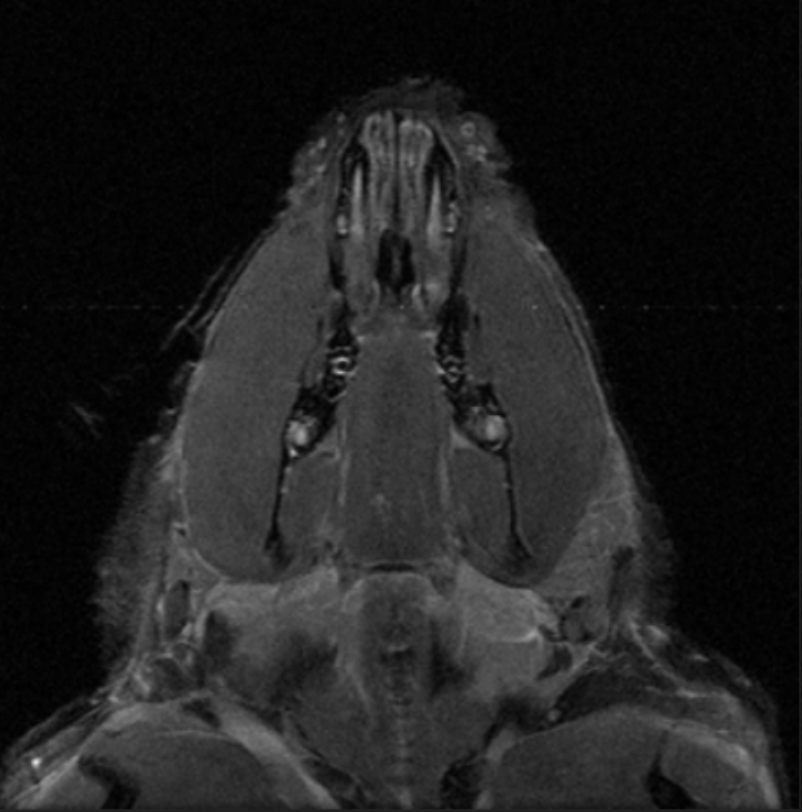
\includegraphics[width=0.47\linewidth]{head-region.png}
    \hfill
    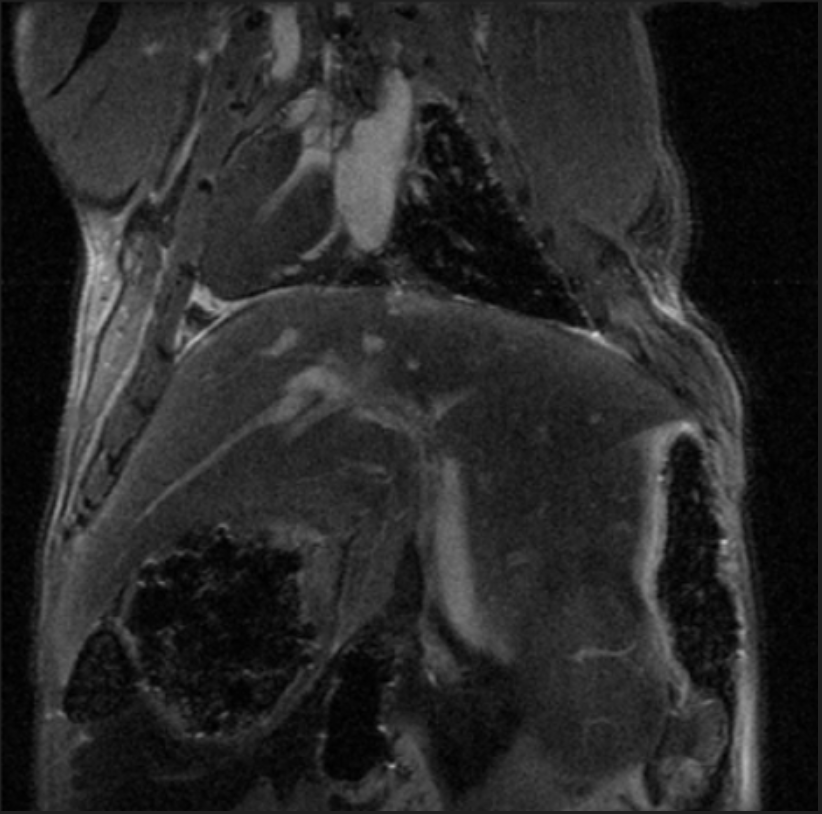
\includegraphics[width=0.47\linewidth]{thorax-abdomen.png}
    \caption{MRI scan regions: head-thorax (left) and thorax-abdomen (right).}
    \label{fig:scan-orientations}
\end{figure}



The acquisition sequence consisted of multiple steps to fine-tune the system before image acquisition began: 

\begin{enumerate}
\item svWobble scan: svWobble was only performed at the start of the first scan session. It helps the system determine how much water is present in the coil and fine-tunes the scanner accordingly. 
This step is especially necessary when switching between different animal species, as the water content in the coil may vary. 
If the same type of sample (e.g., the same mouse model) is used throughout the experiment, svWobble does not need to be repeated for following scans.
\item Tripilot scan:  short, preliminary scan that allows the user to define the field-of-view (FOV) that needs to be acquired. 
This step generates 3 orthogonal views: axial, sagittal and coronal. A bounding box is then manually defined to encompass the required FOV, ensuring the right structures are within the FOV. 
Especially important is the phase direction, where the FOV must cover the entire subject.
\end{enumerate}

\begin{figure}[h!]
\centering
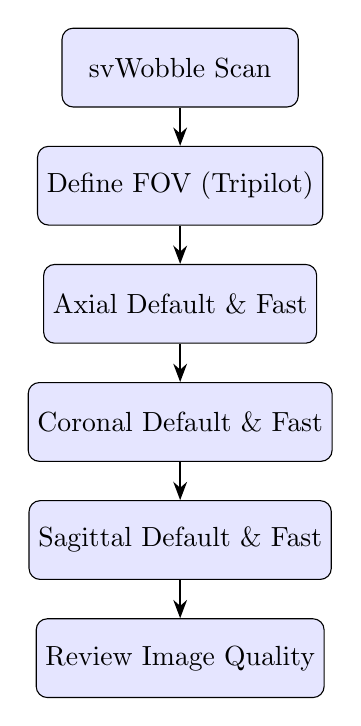
\begin{tikzpicture}[node distance=1.5cm]

\node (start) [process] {svWobble Scan};
\node (fov) [process, below of=start] {Define FOV (Tripilot)};
\node (axial) [process, below of=fov] {Axial Default \& Fast};
\node (coronal) [process, below of=axial] {Coronal Default \& Fast};
\node (sagittal) [process, below of=coronal] {Sagittal Default \& Fast};
\node (review) [process, below of=sagittal] {Review Image Quality};

\draw [arrow] (start) -- (fov);
\draw [arrow] (fov) -- (axial);
\draw [arrow] (axial) -- (coronal);
\draw [arrow] (coronal) -- (sagittal);
\draw [arrow] (sagittal) -- (review);

\end{tikzpicture}
\caption{Schematic overview of the MRI acquisition pipeline.}
\label{fig:acquisition_pipeline}
\end{figure}


\subsection{Performing the MRI scan}
Once the mouse was correctly positioned and the FOV was defined, the process of acquiring 3D MRI data was started. 
This was done for each mouse for both the head-thorax region and the thorax-abdomen region. 
To obtain matched high-low resolution data in all directions, the following sequence was performed: axial default, axial fast, coronal default, coronal fast, sagittal default and lastly sagittal fast. 
In this case ``default'' stands for a 12-minute scan and ``fast'' for a 1-minute scan as can be seen in table ~\ref{tab:mri}.
After each image sequence is completed, they are reviewed to check for any misalignment, artifacts, or other issues to ensure accuracy and quality. 

All scans were acquired using a T2-weighted RARE (rapid acquisition with refocused echoes) sequence. 
This sequence is often used in preclinical imaging because it produces images that have high contrast between different soft tissues. 
T2-weighted images highlight  differences in transverse relaxation time, which reflects how quickly protons lose phase coherence after excitation by a radio frequency pulse. 
This signal decay changes depending on its interaction within different types of tissues. 
Shorter T2's, found in tissues such as muscle and fat, mean that the signal will decay very fast while tissues with a longer T2, for example fluids, retain the signal longer. 
As a result, in fluids appearing brighter than muscle and fat in the image. 

From a technical perspective, the T2-weighted contrast is created by selecting an appropriate echo time (TE) and repetition time (TR). 
The echo time is the time between the initial radio frequency pulse and the measured MRI signal. 
A longer TE allows more time for tissues with a short T2 to lose their signal, resulting in them looking darker on the image. 
Tissues with longer T2 values maintain more signal and will look brighter. Repetition time (TR) refers to the time between successive excitations of the same tissue slice. 
Specifically for T2-weighted images, a longer TR is used, minimizing the influence of T1 relaxation. For this study a TE of 37.1ms and TR of 4000ms are used. 
This provides a strongly T2-weighted image \cite{mrimaster2024} \cite{chavhan2009t2star}.  


\subsection{Image Datasets}

In table ~\ref{tab:mri} the parameters can be found, which were used for the 1-minute low resolution and 12-minute high resolution scans. 
These values were selected in function of the desired acquisition time, image quality and SNR. 
The matrix size determines the level of detail in an image with the high-resolution scan (300x300 pixels) capturing finer structures compared to that of the low-resolution scan (150x150 pixels). 
Other parameters such as repetition time, echo time and thickness remained constant for consistency. The field of view also stays the same at 3 cm x 3 cm to capture the same region of interest. 
An important difference between the two scans is the in-plane resolution. The lower this value, the higher resolution the visualisation. 
The 12-minute scan (0,01 cm/pixel) is more precise while the 1-minute scan (0,02 cm/pixel) is faster but has less detail. 
To significantly enhance SNR by reducing noise, the high-resolution scan uses five averages per slice.\\
\\
In the summer of 2024 an internship was done by Verhelst Niels and Courtens Joran \cite{verhelst2025denoising}. 
The data that they acquired was used in combination with the data acquired in this project. During the internship, 19 mice were scanned. 
In the project, the data of 5 mice were acquired.
 

\begin{table}[h]
\centering
\caption{\label{tab:mri} Overview of the scan and image parameters used to acquire high- and low-resolution data of mice.}
\resizebox{0.8\linewidth}{!}{
\begin{tabular}{l|c|c}
\toprule
 & \textbf{1 min (low-res)} & \textbf{12 min (high-res)} \\
\hline
\midrule
Number of slices & 30 & 30 \\
Matrix size & 150x150 & 300x300 \\
Repetition time & 4000 ms & 4000 ms \\
Field-of-view & 3 cm x 3 cm & 3 cm x 3 cm\\
Echo time & 37.1 ms & 37.1 ms \\
In-plane resolution & 0.02 cm/pixel & 0.01 cm/pixel \\
Slice thickness & 0.6 mm & 0.6 mm \\
Averages per slice & 1 & 5 \\
\bottomrule
\end{tabular}
}
\end{table}

In total, 24 mice (19 + 5) were acquired each in two regions (head-thorax and thorax-abdomen) along three views (coronal, sagittal and transaxial), resulting in a total number of datasets of 24 * 2 * 3 = 144, that can be used for the development of the DL model


\section{Pre-processing and data augmentation}

Pre-processing of the slices is a crucial step in preparing the data for the deep learning model. 
This stage ensures the data is uniform and optimized for training. 

\subsection{Removal of bad image slices}

Some of the obtained images contained artifacts or noise, these could negatively impact the model training. 
To remove these bad slices from the data set, a visualization script was used to display the MRI slices allowing for manual inspection. 
Once bad slices were identified, they were removed from the used dataset (see appendix \ref{Appendix: Figures Preprocessing}: Figure~\ref{fig:bad_slice}). Of the 900 slices acquired, 111 were excluded.

\subsection{Cropping of the image slices}

Cropping is a commonly used image-manipulation process. The obtained MRI images contained lots of background noise which interferes with the performance of the model. 
To counter this problem the images were cropped ensuring that our region of interest was intact (see appendix \ref{Appendix: Figures Preprocessing}: Figure~\ref{fig:comparision-cropped}).  

\subsection{Zarr arrays}

The acquired data were first converted into Zarr arrays to compress the large volume of data while maintaining image quality. 
Unlike other formats this enables faster access since specific slices can be loaded instead of the entire dataset.
The low-resolution image were upsampled using nearest-neighbor interpolation (order=0) with a zoom factor of 2 to match the high-resolution image dimensions. 

\subsection{Normalization}

Mean normalization was performed, each low-resolution image was divided by its mean intensity, and the same mean value was applied as a normalization factor for the corresponding high-resolution image.  
Both low-resolution and high-resolution images were converted for compatibility with PyTorch models.

\subsection{Padding and random flipping}
The images were randomly flipped horizontally and vertically with a 50\% probability, to introduce variations.
This is done during network training. 
This improves the model generalization. Since input may have varying dimensions, the images were padded to match the largest width and height within each batch, ensuring uniform sizes for batch processing.


\section{Neural Network and Training Process}
\subsection{Model architecture}
For the denoising deep learning model, a convolutional neural network based on the U-Net architecture was used. 
U-Net is a form of autoencoder, consisting of two main parts: an encoder and a decoder (see Figure~\ref{fig:U-Net}) \cite{ronneberger2015unet}.

The input to the network is a low-resolution ($150 \times 150$ pixels), which is first upsampled via interpolation to match the high-resolution target size ($300 \times 300$ pixels). 
The network then processes this input to produce a denoised output with a higher signal-to-noise ratio (SNR).

The encoder comprises a series of convolutional layers followed by downsampling steps (e.g., pooling or strided convolutions). 
These layers extract hierarchical features while reducing spatial resolution and increasing the number of feature channels.

The decoder mirrors the encoder structure and consists of upsampling layers (e.g., transposed convolutions or interpolation followed by convolution) that reconstruct the spatial resolution of the input. 
To preserve spatial information and enhance feature propagation, **skip connections** are added between corresponding layers of the encoder and decoder. 
These allow the decoder to directly access feature maps from earlier stages in the encoder, improving the model’s ability to recover fine details.

In this implementation, residual learning is optionally used—not between intermediate layers, but globally between the input and output of the network. 
This means the model learns to predict the residual (i.e., the noise component), which is then added back to the input to reconstruct the denoised image.
This technique can lead to faster convergence and improved stability, as the network focuses on learning the difference rather than the full image content.

The rationale behind using this U-Net structure is that the encoder condenses and abstracts the relevant features of the input image, while the decoder reconstructs an enhanced version by combining this condensed representation with spatially detailed information from the skip connections.

%better resolution image for the unet
\begin{figure*}
    \centering
    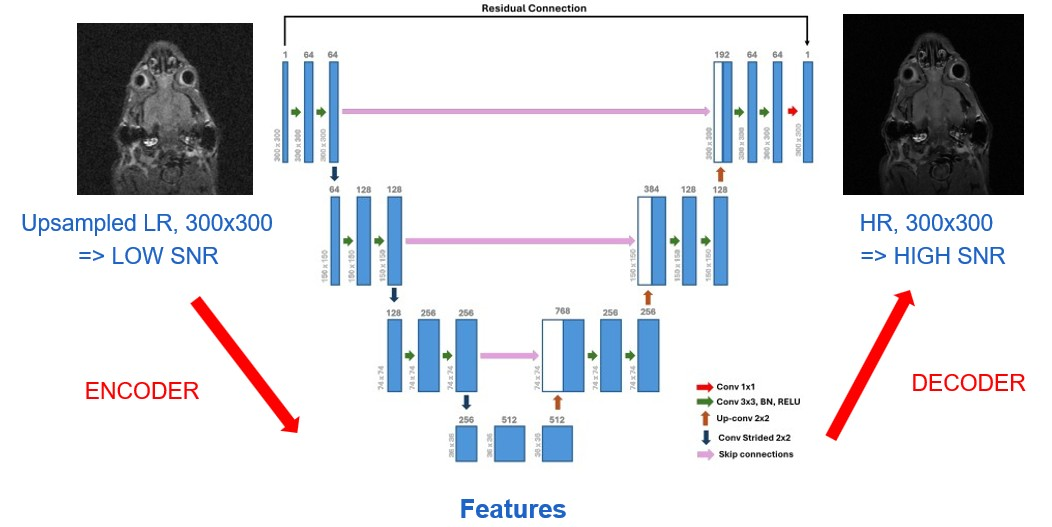
\includegraphics[width=0.8\linewidth]{U-Net.jpg}
    \caption{U-Net architecture.}
    \label{fig:U-Net}
\end{figure*}


\subsection{Encoder-Decoder Model: Hyperparameter Optimization}
To get the best results for the deep learning model for micro MRI image denoising and super-resolution, the hyperparameters need to be fine-tuned. 
Given the number of components and interactions within the model, manual tuning would be inefficient and inconsistent. 
Therefore, an open-source optimization software, such as Optuna, was used \cite{datacamp_optuna}. 

Each trial corresponds to the training of the model with a specific set of hyperparameters. 
The performance metrics are recorded after each trial, for example a validation loss. These metrics are used as a guide for the search. 
A built-in sampler selects new parameter values to explore, while a pruners stops trials early if the model is clearly not improving. 
This combination is especially helpful to reduce the number of trainings that need to be run, this saves computational resources. 

One of the advantages of Optuna is its define-by-run approach \cite{10.1145/3292500.3330701}. 
This means that instead of predefining the entire parameter space before the optimization, the search space is defined dynamically while being executed. 
This gives more flexibility especially in cases where certain parameters are only relevant under specific conditions. 
Instead of testing all combinations blindly, Optuna can selectively explore subsets of the parameter space based on earlier decisions within the same trial. 
The avoidance of meaningless testing makes the optimizations process  more efficient. 

Overall Optuna played a key role in helping reach a well-performing model more efficiently, and ensured that our final configuration was based on data-driven search rather than trial and error.

In summary, the hyperparameter optimization explored a wide variety of configurations for the network structure. 
However, to ensure a fully optimized model, it is equally important to fine-tune the training process itself.
Section \ref{hyperparameters training} extends the optimization to parameters such as learning rate, scheduler strategies, optimizers, loss functions, and training routines. 
This combined approach ensures that both the network architecture and its learning dynamics are tailored to get the best denoising performance. 

\subsubsection{Hyperparameters of the Network Structure }
\paragraph{Features main and features skip}
To determine the number of main features, different powers of 2 were explored. Each component of the \texttt{features\_main} list was assigned a different power of 2, and subsequent elements followed incrementally higher powers. 
The number of elements in this list determines both the depth of the network and the number of feature channels at each layer. 
While sometimes overlooked, these are in fact fundamental architectural hyperparameters, as they define the model’s capacity and depth. 
Therefore, they were explicitly included in the optimization process to assess their impact on performance.

For the \texttt{features\_skip}, the same values as in \texttt{features\_main} were used, but with the last element removed.  
These values define how many filters are used in each layer of the encoder and decoder.  
The skip connections pass feature maps from the encoder to the decoder at corresponding levels, helping the model retain spatial information during reconstruction.

To test different configurations, one value was selected from each of three predefined categories.  
Specifically, \texttt{features\_main\_1} was chosen from [32, 64, 128], \texttt{features\_main\_2} from [64, 128, 256], and \texttt{features\_main\_3} from [128, 256, 512].  
This setup allowed us to systematically explore various combinations of feature sizes and evaluate their influence on model performance.


\paragraph{Downsampling method}
The downsampling method is an important aspect of the encoder and determines how the images will be reduced. Different methods were considered such as maxpooling, meanpooling and strided convolution.  
Maxpooling selects the maximum value from each patch in the feature map, preserving the most prominent features while reducing spatial dimensions. 
This concept can be observed in Figure ~\ref{fig:maxpool} \cite{dhanushkumar-2023}.
Another approach is Meanpooling. Instead of taking the prominent feature, this method averages the values within a patch, offering a smoother downsampling method. 
In Figure ~\ref{fig:meanpool} the concept of meanpool can be seen.
The last method, is strided convolution. The principle can be seen in Figure ~\ref{fig:convStrided}. 
In this approach, the convolution is applied with a larger stride, which determines how far the filter moves across the feature map during the convolution process.
When the stride is greater than 1, the convolution operation skips some of the pixel, which results in an effective method to reduce the size of the feature map \cite{unknown-author-no-date2}.
Each of these methods reduce the size of the feature map but with different strategies.


\begin{figure}
    \centering
    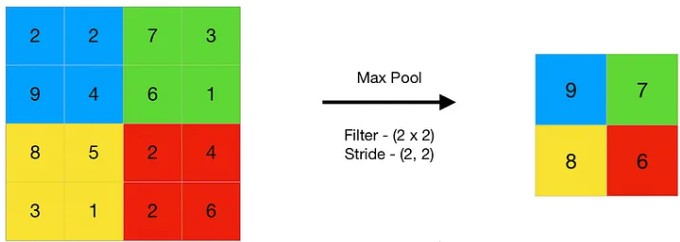
\includegraphics[width=1\linewidth]{Maxpool.jpg}
    \caption{Downsampling - Maxpool}
    \label{fig:maxpool}
\end{figure}

\begin{figure}
    \centering
    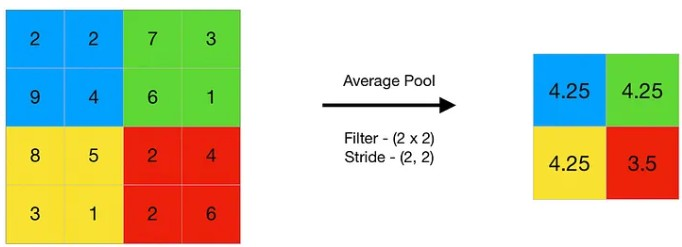
\includegraphics[width=1\linewidth]{Meanpool.jpg}
    \caption{Downsampling - Meanpool}
    \label{fig:meanpool}
\end{figure}

\begin{figure}
    \centering
    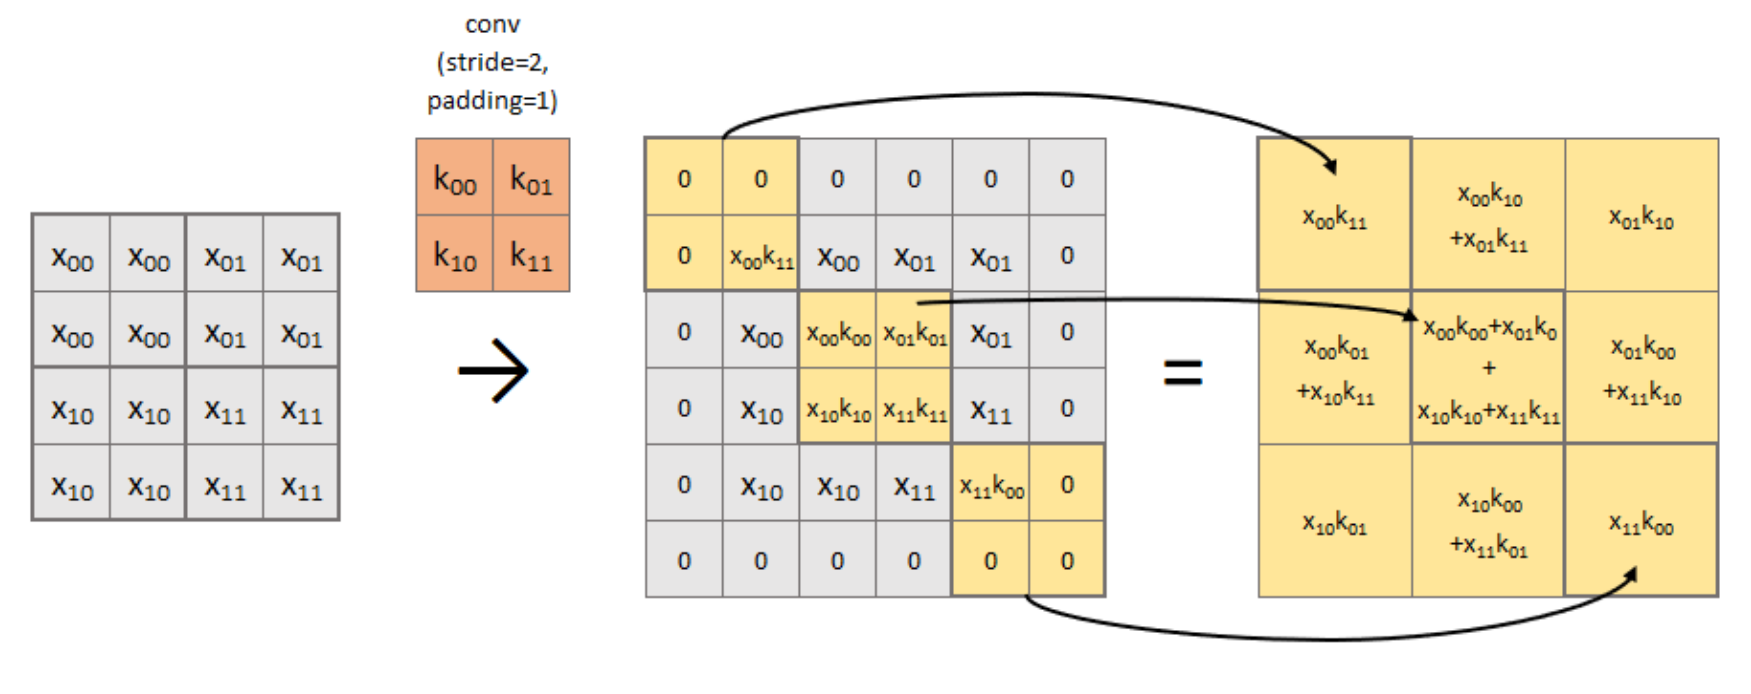
\includegraphics[width=1\linewidth]{ConvStrided_new.png}
    \caption{Downsampling - convStrided}
    \label{fig:convStrided}
\end{figure}


\paragraph{Upsampling}
The upsampling method is the process in the decoder by which the resolution of an image is increased while minimizing the loss in image quality. 
The goal is to increase the number of rows and/or columns of the image. 
Several methods are available, including nearest neighbor, linear, bilinear, trilinear, and bicubic interpolation, as implemented in PyTorch's interpolation modes.

The nearest neighbor interpolation is the simplest approach. 
Each pixel of the upscaled image is assigned the value of its nearest neighbor in the original image. 
This method is fast and simple, but might produce pixelated images.

The linear interpolation calculates the new pixel value by taking a weighted average of the two nearest pixels along a single axis. 
The bilinear interpolation calculates a weighted average of the four nearest neighbors' pixel values in the original image. 
It uses linear functions and a $2 \times 2$ pixel grid. 

The trilinear interpolation is used in 3D images. 
The interpolation is first performed linearly along one axis, followed by linear interpolation along the second and third axes. 
The linear, bilinear, and trilinear methods result in smoother images than the nearest neighbor method.

Bicubic interpolation is more advanced. This method first identifies the nearest $4 \times 4$ grid of pixels surrounding the point that needs to be interpolated. 
Then, it calculates the cubic polynomials that best fit the pixel values in the grid. 
After that, the pixel intensity is estimated at the target position. 
It is an effective method for high-quality upscaling because it preserves details and reduces artifacts  \cite{unknown-author-2025} \cite{amanrao-2023}.

\paragraph{Activation function}
Activation functions introduce a non-linearity into the network. This allows complex mapping between inputs and outputs. 
Without an activation function, the network would behave like a linear system and would not be able to model intricate relationships such as edges and contrast. 
Different options were tested such as ReLU,  LeakyReLU, ELU and PReLu. Each of these options come with their own set of advantages and difficulties. 
ReLU (Rectified Linear Unit) is most commonly used as an activation function because of its simplicity and computational efficiency. 
This function \ref{eq:4} returns the positive inputs directly and zero if negative. One of the limitations is a phenomenon called `dying neurons`',  if a neuron only receives negative inputs, it will always output zero and stop learning.
LeakyReLU adresses this problem by allowing small negative outputs. This function \ref{eq:5} helps keeps neurons active and keeping them active. 
This technique keeps the simplicity or ReLU while improving stability. 
ELU is similar to LeakyReLU in sense that negative outputs are generated, but in this case with a smooth exponential curve \ref{eq:6}  instead of a constant curve. 
Finally, PReLU (Parametric ReLU) also starts from LeakyReLU but in this case the negative slope is a learnable parameter and not a fixed value. 
This lets the model adapt the activation function in training leading to potentially better performance. 
However it does introduce an extra parameter increasing computational cost \cite{bharatiya_2019_comprehensive}.

\begin{equation}\label{eq:4}
    f(x)_{ReLU} = \max(0, x)
\end{equation}

\begin{equation}\label{eq:5}
f(x)_{LeakyReLU} = 
\begin{cases}
x & \text{if } x \geq 0 \\
\beta x & \text{if } x < 0
\end{cases}
\end{equation}

\begin{equation}\label{eq:6}
f(x)_{ELU} = 
\begin{cases}
x & \text{if } x \geq 0 \\
\alpha (e^x - 1) & \text{if } x < 0
\end{cases}
\end{equation}


\begin{equation}\label{eq:7}
f(x)_{PReLU} = 
\begin{cases}
x & \text{if } x \geq 0 \\
a x & \text{if } x < 0
\end{cases}
\end{equation}

\paragraph{Residual learning}
With residual learning instead of predicting the final high-resolution images the model learns the difference between the low- and high-resolution, this is called the residual. 
After training, the residual is added back onto the input image to produce the final image. This method has its advantages. 
Learning the missing information is often faster and easier than predicting the entire image. This can lead to faster and better convergence. 
In this project residual learning is an optional feature, which can be set True or False. Optuna was used to explore if enabling led to better performance.

\subsubsection{Hyperparameters of the Training Process}\label{hyperparameters training}

\paragraph{Learning Rate Strategies} \label{subsec:LearningRateStrategies}
The scheduler adjusts the learning rate during training according to a predefined strategy.  
The following schedulers were tested: exponential learning rate (\texttt{ExponentialLR}), step learning rate (\texttt{StepLR}), and reduce learning rate on plateau (\texttt{ReduceLROnPlateau}).

The \texttt{ExponentialLR} divides the learning rate every epoch by the same factor $\Gamma$.  
As a result, the learning rate decreases quickly during the first epochs and then gradually stabilizes, approaching zero over time.  
\texttt{StepLR} is similar to \texttt{ExponentialLR}. It also decays the learning rate by gamma. However, the key difference is that this decay occurs only every $N$ epochs.  
This leads to more gradual and less frequent reductions in the learning rate compared to \texttt{ExponentialLR}.  
Their respective formulas \ref{eq:1} and \ref{eq:2} are given below.

Another scheduler is \texttt{ReduceLROnPlateau}. Unlike the others, it adapts the learning rate based on the performance of a specified metric.  
This algorithm decreases the learning rate when the specified metric stops improving for longer than allowed.  
So, the learning rate is kept constant as long as the metric improves.  
When the learning rate is reduced, the results stagnate \cite{unknown-author-no-date3} \cite{isbhargav-2020}.

These schedulers make use of a learning rate decay value, which determines how much the learning rate is reduced at each step.  
The learning rate decay decreases the learning rate as training progresses and becomes more stable.  
It is used in the scheduler algorithms as the step size.  
Here, the learning rate decay values of 0.1, 0.3, and 0.5 were tested.

In addition to scheduling and decay, selecting an appropriate initial learning rate is also crucial.  
The pace in which the weights are updated during training depends on the learning rate.  
A learning rate value which is too high can lead to instability and poor convergence, while a value that is too low might slow down the training of the model, as shown in Figure \ref{fig:Learnrate}, or even cause the model to get stuck in a local minimum \cite{jordan_2018_setting}.  
Optuna was used to search across a continuous range of values \([10^{-2}, 10^{-6}]\) to find the optimal balance between convergence and stability.

\begin{equation}\label{eq:1}
lr_{\text{epoch ExponentialLR}} = \Gamma \times lr_{\text{epoch}-1}
\end{equation}

\begin{equation}\label{eq:2}
\resizebox{1.\hsize}{!}{$
lr_{\text{epoch}} =
\begin{cases}
\Gamma \times lr_{\text{epoch}-1}, & \text{if } \text{epoch} \bmod \text{step\_size} = 0 \\
lr_{\text{epoch}-1}, & \text{otherwise}
\end{cases}
$}
\end{equation}

\begin{figure}
    \centering
    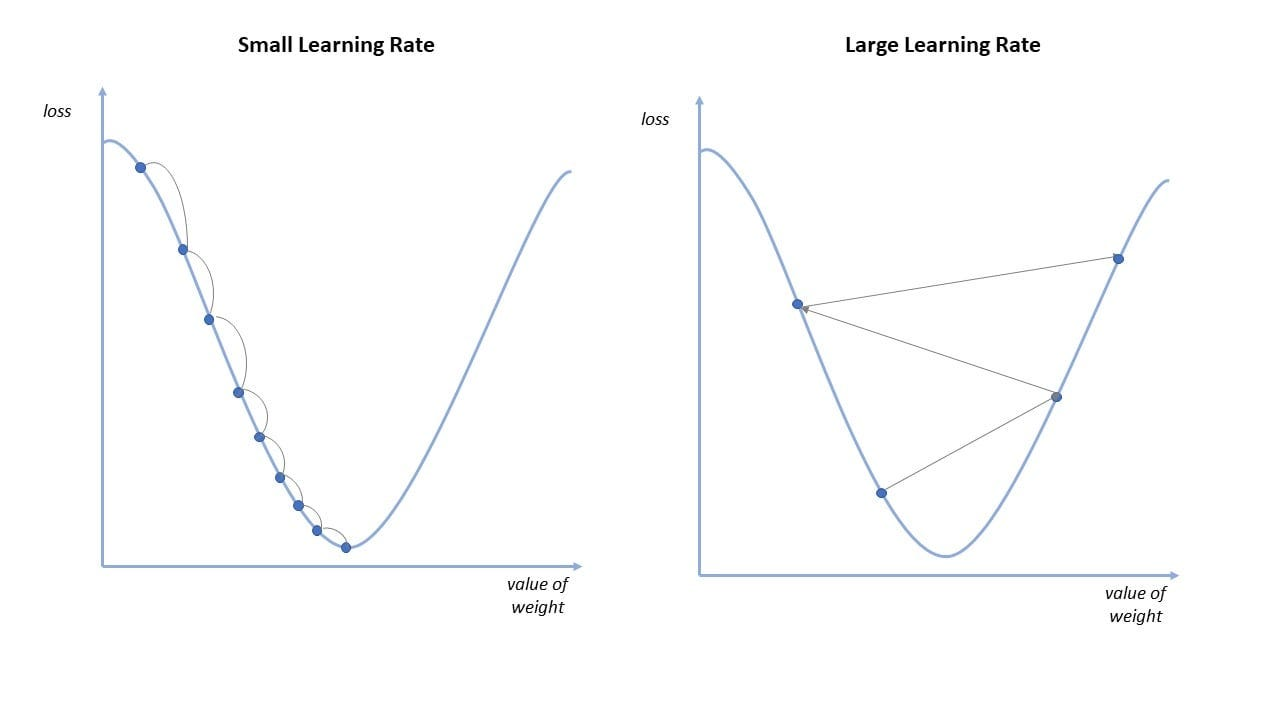
\includegraphics[width=1\linewidth]{Learn rate.jpg}
    \caption{Comparison of different learning rates}
    \label{fig:Learnrate}
\end{figure}

\paragraph{Optimizer}
The optimizer plays a crucial role in fine-tuning the model's weights during training to minimize the loss function. 
Different methods are available, each with its own advantages and disadvantages. 
In this project, four different optimizers will be tested: Adam, AdamW, SGD and RMSprop. 
One of its limitations is the way it incorporates L2 regularization directly into the gradient update, which can sometimes negatively affect the performance. 
Stochast gradient descent(SGD) updates the model’s parameteres basedon the gradient loss function. Unlike Adam, ituses a fixed learning rate and does not estimatemoments of the gradients
In contrast, AdamW decouples weight decay from the gradient update, applying it separately after the parameter update, which provides a more effective approach \cite{pykes-2021}.
RMSprop, also known as root mean square propagation, is another gradient-based optimization algorithm. It uses a moving average of the squared gradients to adapt the learning rate for each parameter. 
This means it does not rely solely on the current gradient, but also incorporates information from previous updates. By "remembering" the magnitude of recent gradients, RMSprop smooths out noisy updates and helps stabilize the training process. 
This leads to faster and more reliable convergence, particularly in settings with sparse gradients or noisy data, functioning similarly to momentum-based methods.
It uses an adaptive learning rate instead of treating the learning rate as a hyperparameter, which results in a change of learning rate over time. 
This can result in faster convergence \cite{sanghvirajit-2025}.



\paragraph{Loss function}\label{loss_function}
The loss function defines how well our model is performing by evaluating the prediction against the target images. 
It guides the process by providing a measure of error which then can be minimized during training. 
3 loss functions were tested: Mean Squared Error (MSE) , Mean Absolute Error (MAE) and a hybrid loss. 
MSE penalizes the squared difference between the predicted and true pixel values. 
This loss function penalizes large errors more severely because the errors are squared. 
This method is effective for achieving high numerical accuracy but can lead to overly smooth outputs with less fine structural detail.
MAE computes the average of the absolute differences between predicted and true pixel values. 
This method preserves edges and sharper transitions better than MSE but it is less sensitive to small errors and can converge more slowly \cite{anderson_2023_loss}.
The last option, the hybrid loss, is a custom-defined loss which combines mean squared error (MSE) and structural similarity index (SSIM).
\begin{equation}\label{eq:3}
\mathcal{L}_{\text{hybrid}} = \alpha \cdot \mathcal{L}_{\text{MSE}} + (1 - \alpha) \cdot (1 - \text{SSIM})
\end{equation}
\begin{itemize}
    \item $\alpha \in [0, 1]$ controls the balance between the two components,
    \item $\mathcal{L}_{\text{MSE}}$ measures the average pixel-wise error between the predicted and ground truth images,
    \item $\text{SSIM}$ evaluates perceptual similarity.
\end{itemize}

The Structural Similarity Index Measure (SSIM) is used to evaluate the perceptual similarity between two images.  
Unlike MSE or MAE, which focus on absolute pixel-wise differences, SSIM compares structural information by considering changes in luminance, contrast, and structure.  
This makes it particularly suitable for applications like medical imaging, where preserving anatomical detail is important.
\begin{equation}\label{eq:SSIM}
\text{SSIM}(A, B) = \frac{(2 \cdot \mu_A \cdot \mu_B + c_1)(2 \cdot \sigma_{AB} + c_2)}{(\mu_A^2 + \mu_B^2 + c_1)(\sigma_A^2 + \sigma_B^2 + c_2)}
\end{equation}

\begin{itemize}
    \item $\mu_a,\mu_b$ : mean intensities of images A and B
    \item $\sigma_A^2, \sigma_B^2$ :variances
    \item $\sigma_{AB}$ : covariances
    \item $c_1,c_2$ : 2 variables which stabilize the division (both are typically small values)
\end{itemize}

MSE helps preserve pixel-wise fidelity while SSIM ensures structural integrity of the image, which is crucial in medical contexts. 
Optuna was used to choose the type of loss function to apply and, in the case of the hybrid loss, to optimize the value of alpha. 
This allowed the model to adaptively prioritize pixel accuracy versus perceptual quality. 

\paragraph{Others}
Several training-related settings were applied to control the model optimization process, including early stopping, batch size, and the number of training epochs.
While these are not traditional hyperparameters in the architectural sense, they significantly influence model performance and training efficiency.

Early stopping was used to prevent excessive training and potential overfitting. The criterion is based on a `no improvement`' threshold, where training stops if validation performance does not improve for a set number of epochs. 
In this project, training was stopped if no improvement was observed after 6 consecutive epochs, with a minimum of 10 epochs always run to ensure sufficient learning.

Batch size determines how many training samples are processed before updating the model weights. Larger batch sizes provide more stable gradient estimates, which can speed up training but require more memory and may generalize worse. 
Smaller batches introduce more noise into gradient updates, which can help escape local minima but may lead to slower convergence.

Number of epochs refers to how many times the model sees the entire training dataset. Although not a direct hyperparameter, it plays a key role in controlling learning. 
Too few epochs can result in underfitting, while too many may lead to overfitting, especially when early stopping is not properly configured.



\subsection{Anchored Path Diffusion Denoising Model (APDDM)}
To complement the direct image-to-image denoising approach discussed earlier, a second model was implemented: the Anchored Path Diffusion Denoising Model (APDDM). 
This method is based on the original DDPM framework by Ho et al. (2020) \cite{DDPM}. 
A schematic representation can be found in Figure \ref{fig:PDDM} and Figure \ref{fig:APDDM} for PDDM and APDDM, respectively.
Unlike DDPM, which is trained on unpaired data and gradually adds Gaussian noise until the image becomes entirely random, APDDM is adapted for use with paired high- and low-SNR MRI images, in this case, the 12-minute high-resolution scans and the 1-minute low-resolution scans.
Instead of diffusing toward a generic Gaussian distribution, APDDM anchors the diffusion process around the actual low-SNR image. This allows the model to introduce realistic, data-driven noise during training.
Moreover, APDDM does not rely on variational inference, but instead follows a more controlled and interpretable forward process tailored to the dataset.
These changes make it better suited for applications like medical imaging, where noise is often structured and non-Gaussian.

\begin{figure*}
    \centering
    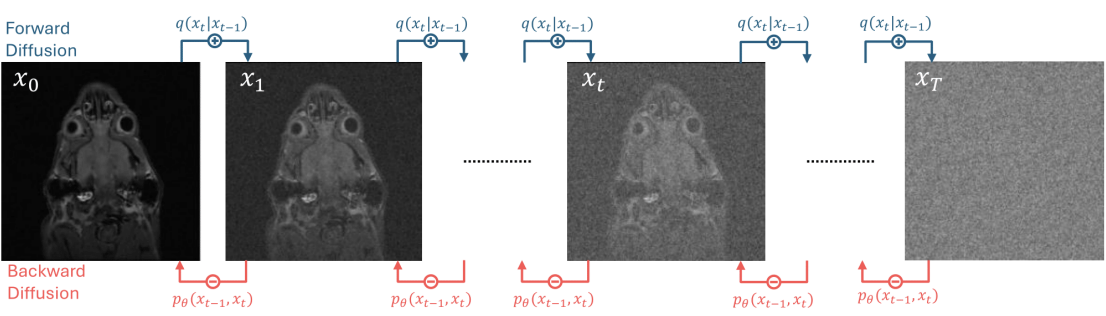
\includegraphics[width=1\linewidth]{DDPM_model.png}
    \caption{Schematic representation of the DDPM model from the Ho et al. paper.}
    \label{fig:PDDM}
\end{figure*}

\begin{figure*}
    \centering
    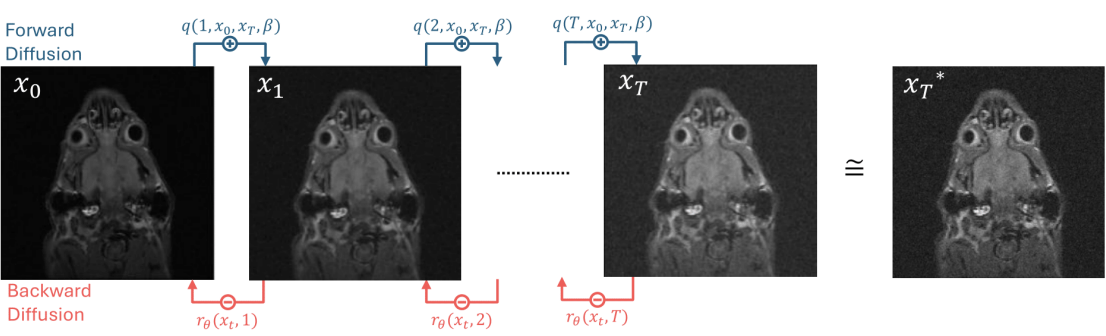
\includegraphics[width=1\linewidth]{ADDPM_model.png}
    \caption{Schematic representation of the ADDPM model.}
    \label{fig:APDDM}
\end{figure*}




\subsubsection{Forward Diffusion Process}
The forward process defines a stochastic path that gradually transforms the clean image $x_0$ into a noisy version $x_t$, with the endpoint distribution anchored around the real noisy scan $x_T^*$. 
This is achieved using a Markov chain defined by:

\begin{equation}\label{eq:Markov chain}
\begin{split}
x_t=q(x_{t-1})=x_{t-1}+\frac{1}{T}\cdot R+f(t)\cdot \hat{\epsilon}\\
t=1,2,...,T
\end{split}
\end{equation}

\begin{itemize}
    \item $R=x_T^*-x_0$ : the residual between 2 paired images
    \item $\hat{\epsilon} $: noise sampled from empirical residuals
    \item $f(t)=4 \cdot \frac{t}{T} \cdot (1-\frac{t}{T})$ : noise schedule function (this can be defined in multiple ways, but a certain choice is made)
    \item $T$ : the total number of diffusion steps
\end{itemize}


The approach guarantees that the endpoint of the forward diffusion $x_T$ is close to the true low-SNR image $x_T^*$. 
By anchoring the path to $x_T^*$, the model maintains connected to the real noise present in the dataset. 
This concept is illustrated in Figure \ref{fig:forward APDDM}. The forward diffusion path (indicated in orange) gradually moves from the high-SNR image $x_0$ toward a distribution centered around the noise image $x_T^*$, with each step adding increasing amount of noise. 


\begin{figure*}[H]
    \centering
    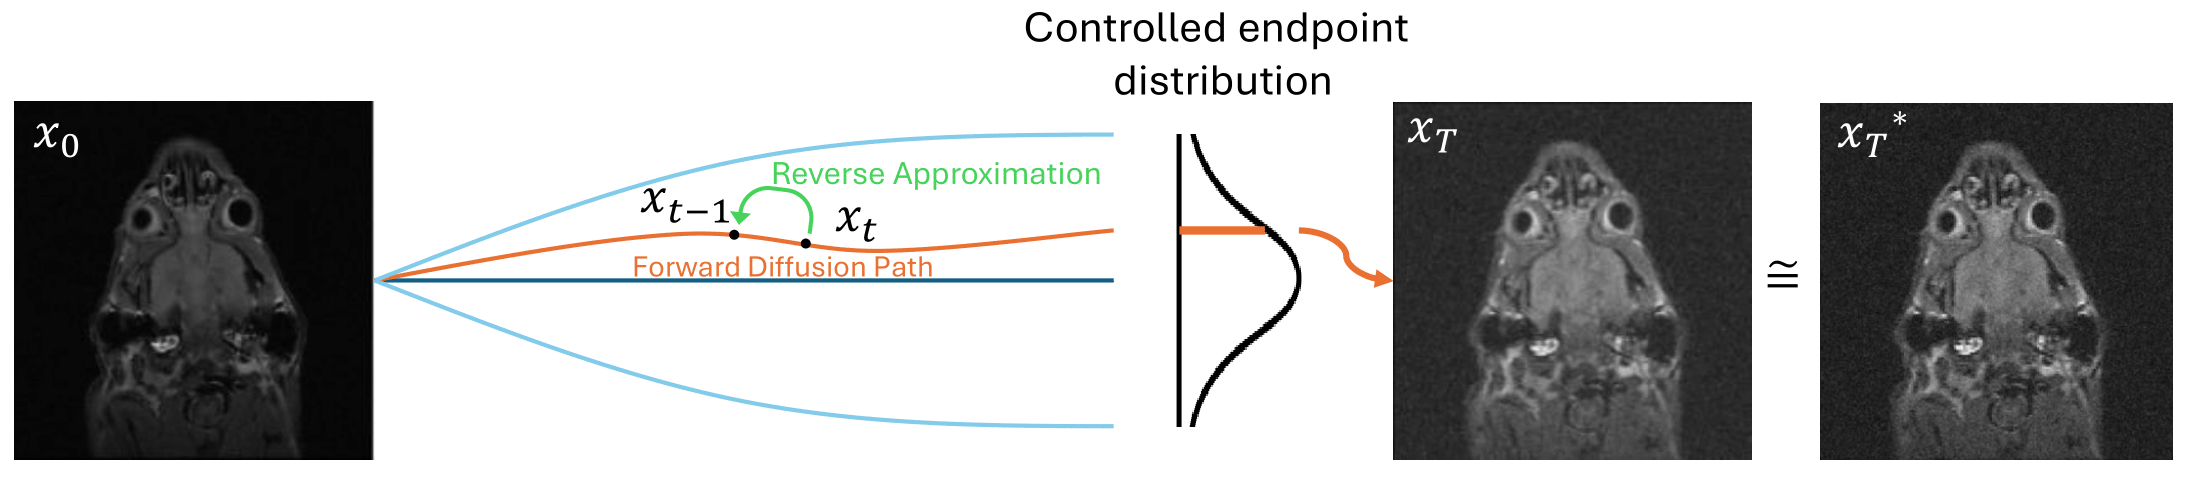
\includegraphics[width=1\linewidth]{forward APDDM.png}
    \caption{forward diffusion APDDM.}
    \label{fig:forward APDDM}
\end{figure*}

\subsubsection{Reverse Process and Training}
To reconstruct $x_0$ from any intermediate $x_t$, a U-Net model $r_{\theta}$ is trained to predict the added noise. 
The predicted noise is then subtracted to obtain an estimate of $\hat{x_0}$, and training is performed using mean squared error loss: 
\begin{equation}\label{eq:Markov chain}
    \hat{x_0}=x_t-f(t) \cdot r_{\theta}(x_t,\frac{t}{T})
\end{equation}
\begin{equation}
    \mathcal{L}=\|x_0-\hat{x_0}\|^2
\end{equation}
The network does not need to generate high-quality images from scratch but only needs to estimate the noise added from the forward process. 
Figure \ref{fig:APDDM} shows the training strategy. The clean image $x_0$ is transformed into $x_t$ via forward diffusion and the network is trained to reverse this transformation by removing predicted noise and minimizing the loss. 
This setup allows the network to focus on denoising realistic degraded images, guided by noise from the data.

\begin{figure*}[H]
    \centering
    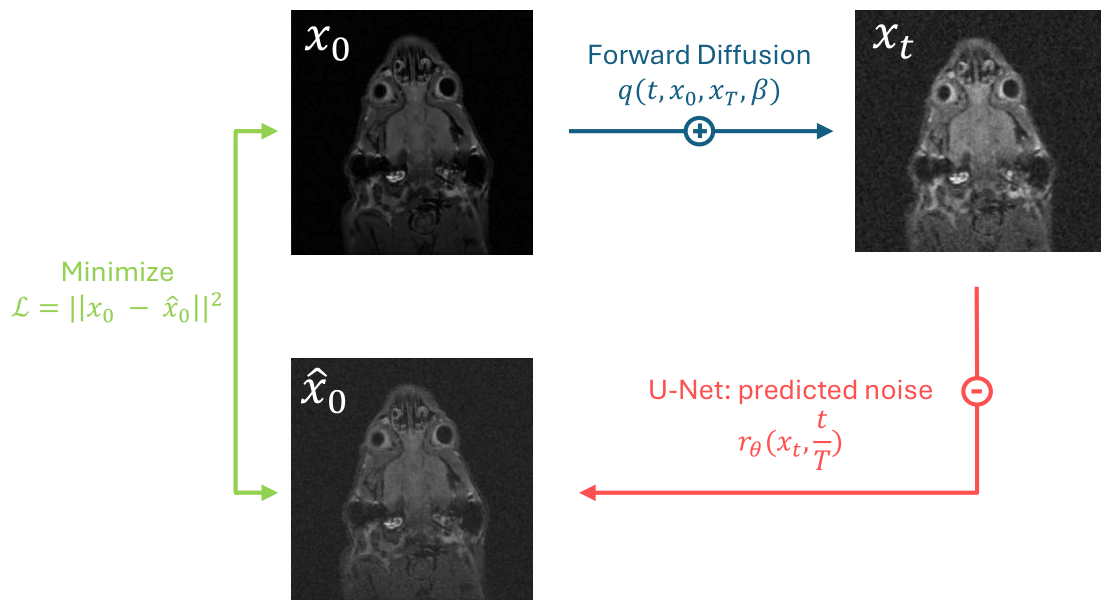
\includegraphics[width=1\linewidth]{full APDDM .png}
    \caption{training overview of APDDM.}
    \label{fig:APDDM}
\end{figure*}

\subsubsection{Integration}
APDDM is particularly well suited for our micro-MRI dataset, where paired scans with varying SNR levels are available. 
By using real residuals between the paired images as noise sample, the forward process creates realistic, data-driven noisy versions of the high-resolution images. 
This ensures that the denoising task is meaningful and well-aligned with the expected variation in practice. 
Furthermore, the ability to modulate noise strength and variance offers great control over training difficulty. 
As an example, increasing noise allows for more challenging samples, improving the model's robustness to varying noise levels in unseen data. 
Overall, APDDM offers a highly customizable framework for modeling noise in paired data and provides a strong foundation for future extensions. 
The mathematical derivations that support this model can be found in Appendix \ref{appendix:Mathematics APDDM}


\section{Model performance evaluation}
In this section, the used validation methods are described. All the methods check the performance of the model. 

\subsection{Visual comparison}
A visual inspection can also be done to evaluate the quality of the reconstructed images. 
The visual comparision will compare the residuals of high-resolution and low-resolution images to the residuals of high-resolution and deep-learning images. 
Ideally the residual of high-resolution and deep-learning images should be close to zero in most regions, indicating an accurate reconstruction. 


\subsection{Mean squared error}
The mean squared error (MSE) measures the amount of error in statistical models by taking the average squared difference between the observed and predicted values. 
If there is no error, the MSE will become zero. Formula \ref{eq:MSE} can be used to calculate the MSE: 

\begin{equation}\label{eq:MSE}
    \text{MSE} = \frac{1}{x \cdot y} \sum_{i=0}^{x-1} \sum_{j=0}^{y-1} \left( S(i, j) - \hat{S}(i, j) \right)^2
\end{equation}

Here, S(i, j) is the observed value, and $\hat{S}(i, j)$  is the corresponding predicted value. 
X represents the number of pixels in a row and y denotes the number of pixels in a column. \cite{mseJim}

The MSE was calculated for the high resolution and the result of the deep learning model. After these calculations the ratio is taken of these two.

\subsection{Structural similarity index measure}\label{Structural similarity index measure}

As previously introduced in section \ref{loss_function}, the Structural Similarity Index Measure (SSIM) is also used independently as an evaluation metric in this study.  
While it forms part of the hybrid loss function, SSIM is valuable on its own for assessing perceptual image quality, as it accounts for luminance, contrast, and structural consistency.
In this context, SSIM is used to compare the predicted images to the high-resolution reference scans.  
This is particularly relevant in medical imaging, where preserving structural details is critical.  
The SSIM score ranges from 0 to 1, with values closer to 1 indicating higher structural similarity and visual fidelity \cite{dosselmann-2009}.

\subsection{Contrast-to-noise ratio}
Contrast-to-noise ratio (CNR) is a metric that evaluates the quality of an image by measuring how well a region of interest (for example, liver) can be distinguished from the surrounding background.
\begin{equation}\label{eq:CNR}
\text{CNR}=\frac{\mu_{ROI}-\mu_b}{\sigma_b}
\end{equation}

$\mu_{ROI}$ is the mean of the region of interest (ROI), $\mu_b$ is the mean of the background and $\sigma_b$ is the noise in the background.
A higher CNR value indicates better differentiation of the region of interest from its background.
To obtain the CNR, the program Amide is used. First, slices were randomly selected from 2 mice in each of the training, validation and test set. For each of these mice, one slice was selected from each anatomical plane-sagittal, transaxial and coronal- resulting in one slice per mouse.
These slices were saved as raw data files, with their shape corresponding shape information. Both were loaded into amide. A ROI of interest was selected and a box was drawn in it. The same procedure was followed for the background region.
Figure \ref{fig:CNR} visualises the procedure described above. 
Next to the CNR, the normalised variation was also calculated. This follows the same procedure as the CNR and is defined as:
\begin{equation}\label{eq:normsigma}
\sigma_{\text{norm}} = \frac{\mu_b}{\sigma_b}
\end{equation}

\begin{figure}
    \centering
    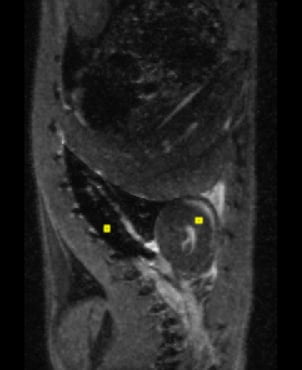
\includegraphics[width=0.35\linewidth]{CNR.jpeg}
    \caption{Example of ROI and background indication}
    \label{fig:CNR}
\end{figure}

\section{Results}
\subsection{First results}
First the model was run on the hpc to check whether all components were implemented correctly. 
With this first run, the pre-processing steps could be verified and the first results could be observed. 
The training was done on the accelgor cluster. 
The 11th epoch was the best, as can be observed in Figure \ref{fig:first_loss}.
In the best epoch the loss of the training is equal to 0.481, while the one of the validation equals 0.426.

\begin{figure}
    \centering
    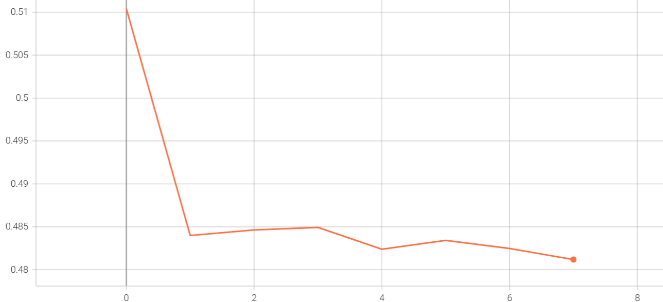
\includegraphics[width=1\linewidth]{First_results_loss.png}
    \caption{Visual representation of the loss function over different epochs. NO AXIS -> change with new figure at PC of Wolf}
    \label{fig:first_loss}
\end{figure}

In this script the training, validation and test mice were defined. A detailed overview can be found in Table \ref{tab:mouse_distribution}.
The hyperparameters were chosen based on knowledge and guessing what the best one would be. They were chosen as followed:
\begin{itemize}
    \item 64 filters in the first layer
    \item 128 filters in the second layer
    \item 256 filters in the third layer
    \item meanpooling for downsampling
    \item upconv upsampling
    \item residual connections
    \item learning rate of 0.0001
    \item RMSprop optimizer
    \item ReduceLROnPlateau scheduler
\end{itemize}
The model was trained with a batch size of 32 and training was conducted over 200 epochs. MSE was employed as the loss function and ReLU was the activation function.


In Figure \ref{fig:first_sagittal}, Figure \ref{fig:first_transax} and Figure \ref{fig:first_coronal} the results can be observed, where each is an example of the training mice. 
Since the output gave not all images back, Figure \ref{fig:first_coronal} is a result of the 13th epoch.
Each image depicts another plane of the mouse. Also, images of the test mice can be found in Appendix \ref{Appendix: first results}

\begin{figure*}
    \centering
    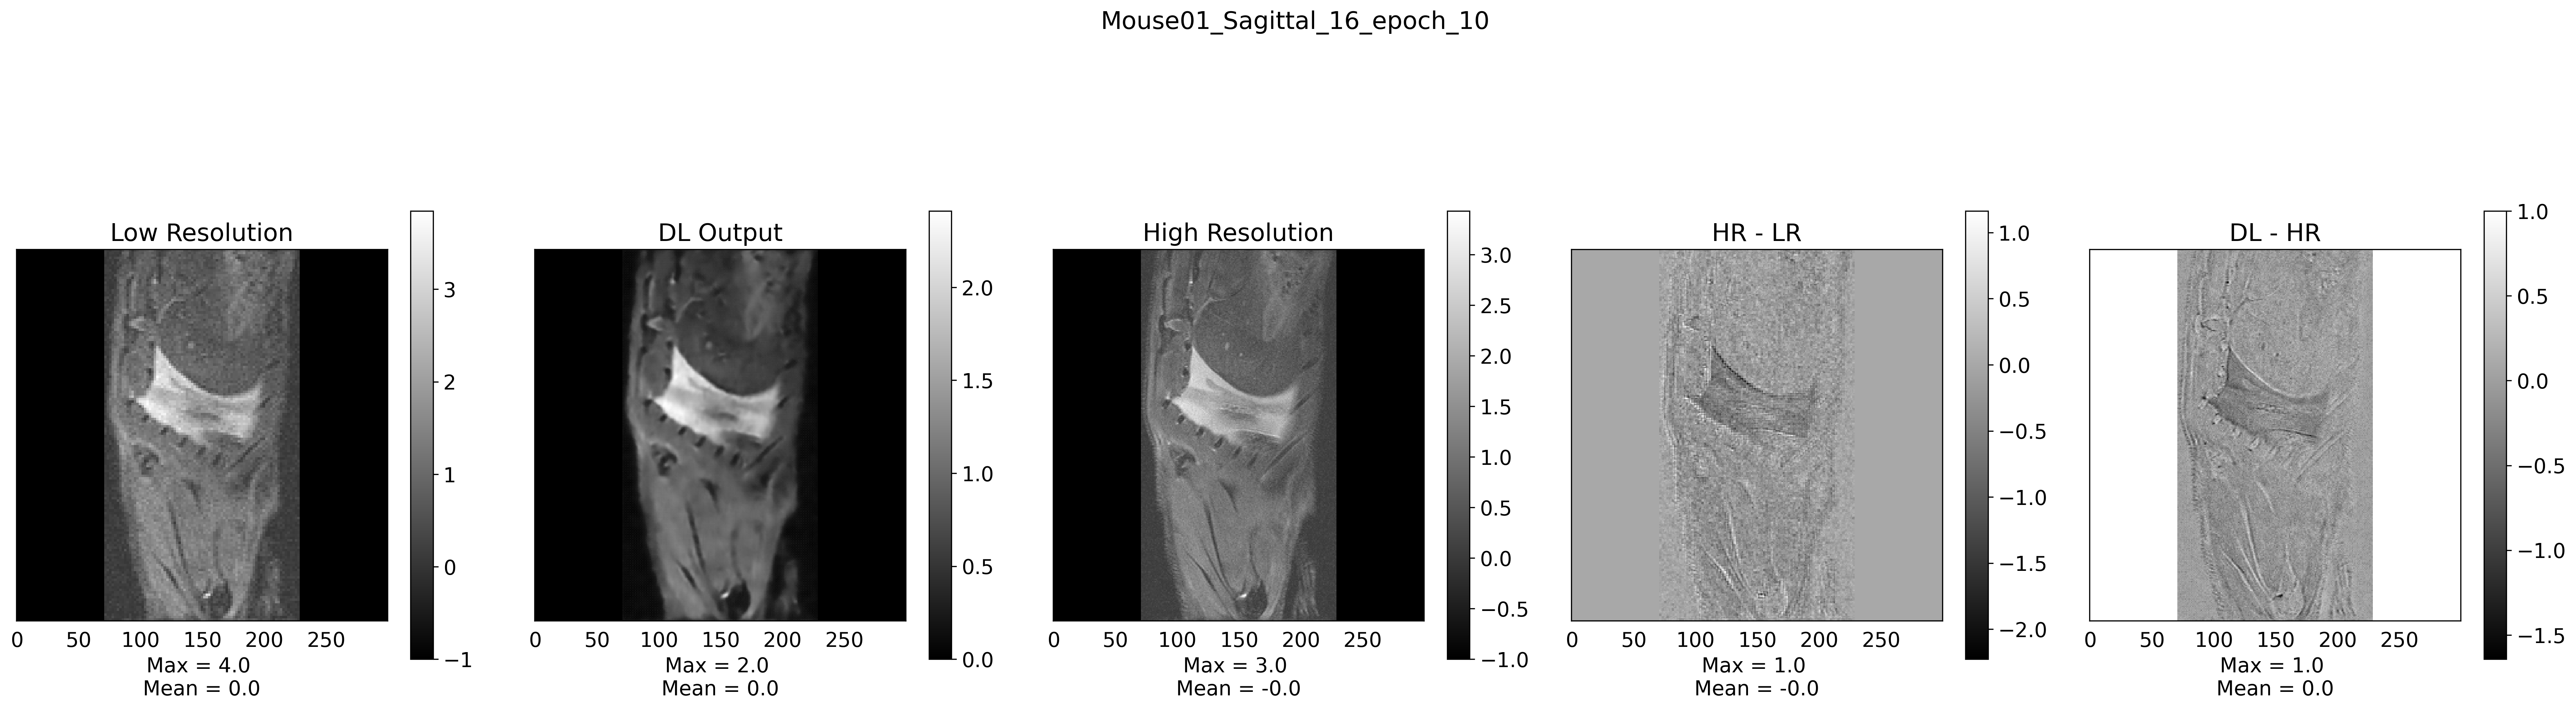
\includegraphics[width=1\linewidth]{Mouse01_Sagittal_16_epoch_10.png}
    \caption{First results of abdomen of training mouse.}
    \label{fig:first_sagittal}
\end{figure*}

\begin{figure*}
    \centering
    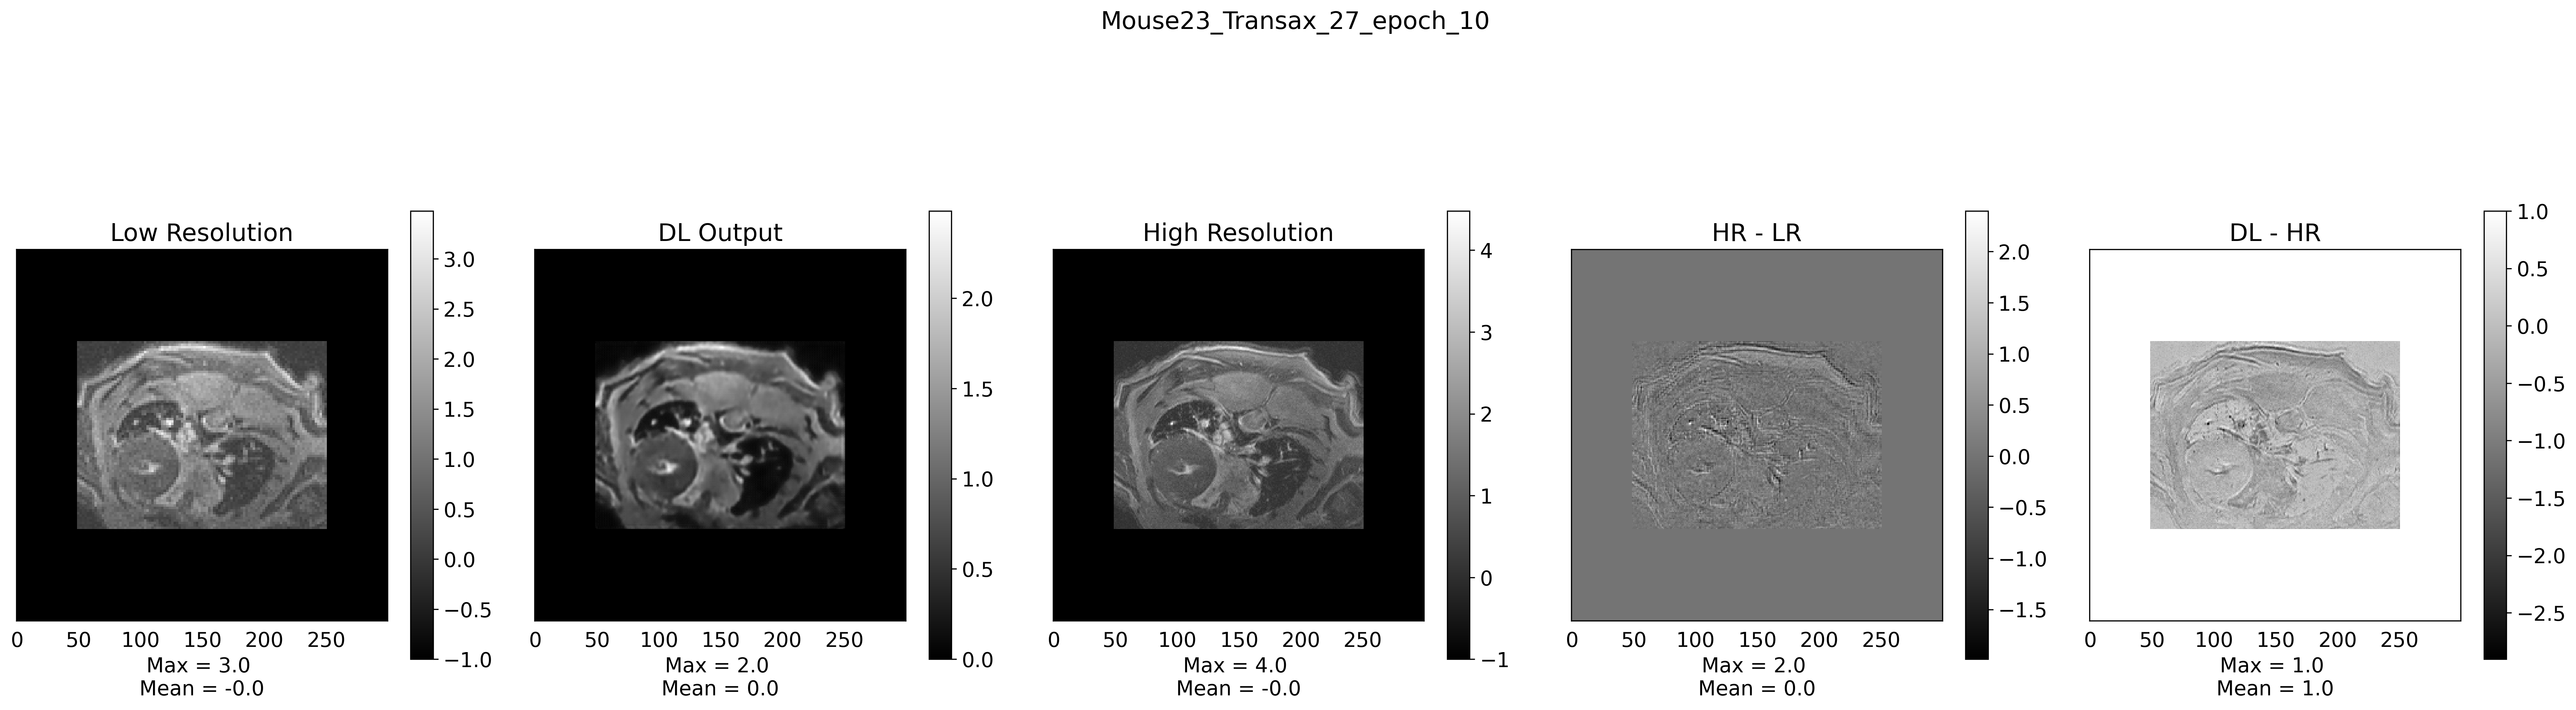
\includegraphics[width=1\linewidth]{Mouse23_Transax_27_epoch_10.png}
    \caption{First results of abdomen of training mouse.}
    \label{fig:first_transax}
\end{figure*}

\begin{figure*}
    \centering
    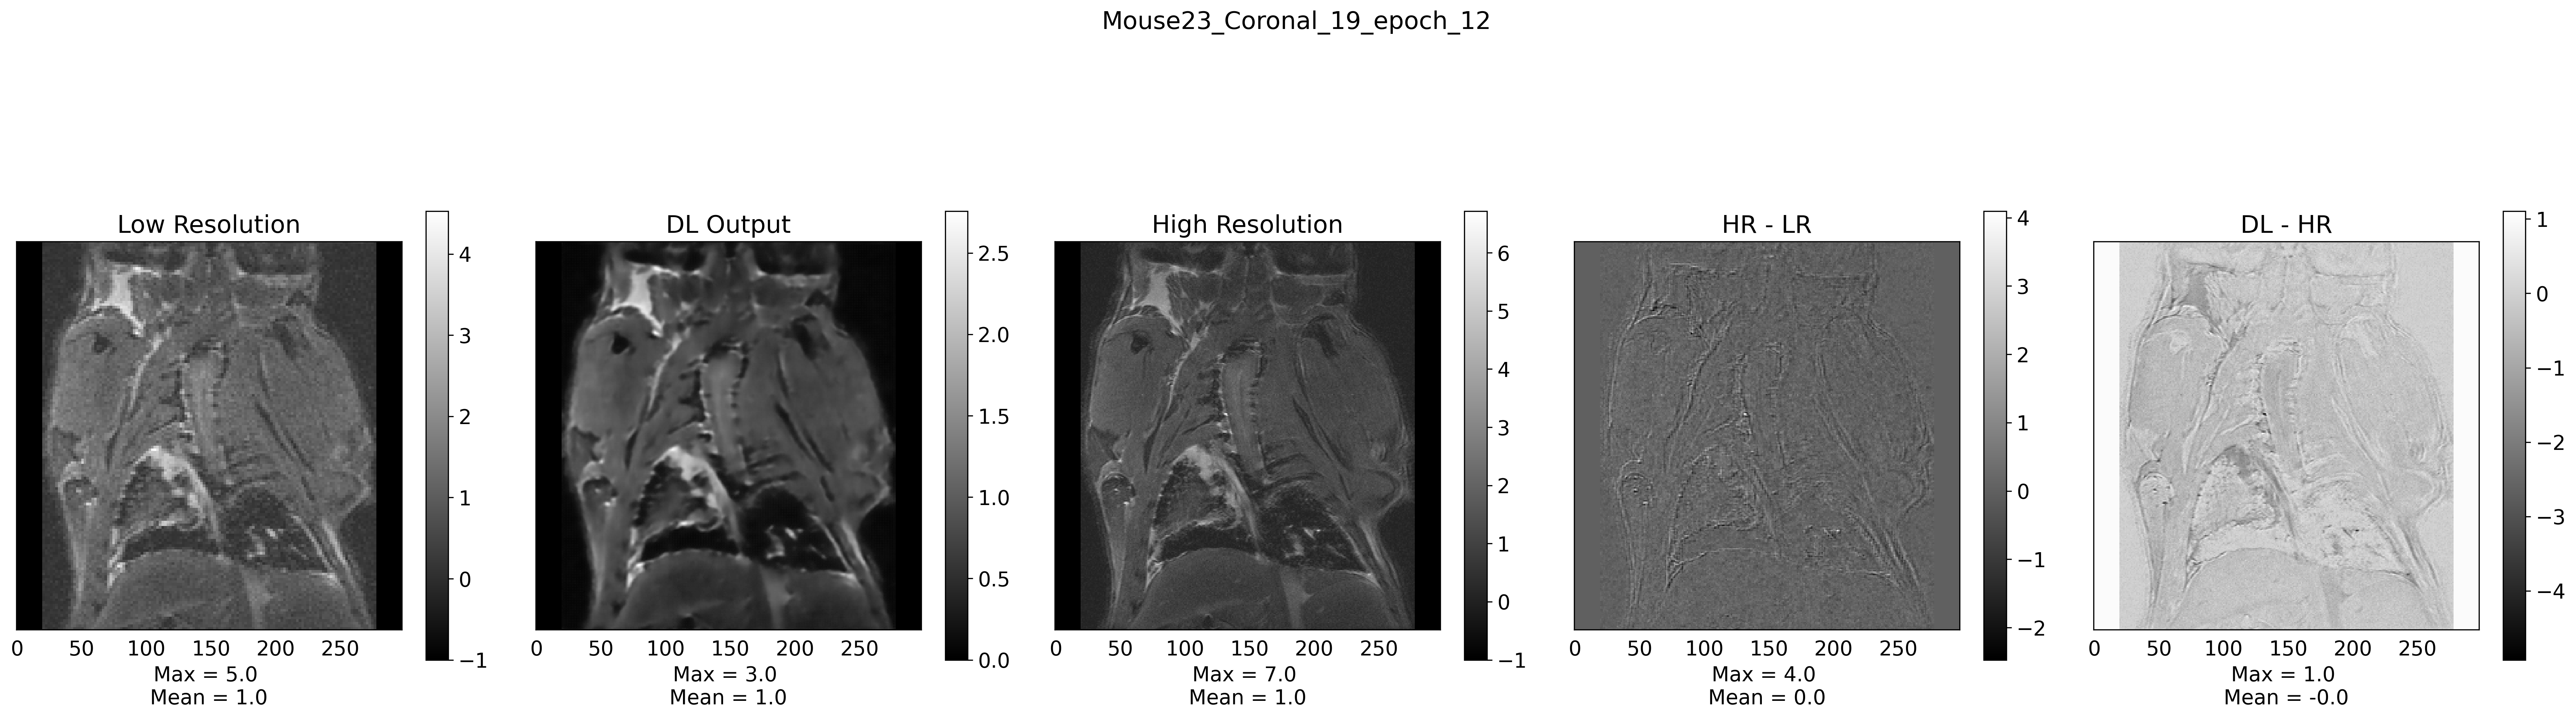
\includegraphics[width=1\linewidth]{Mouse23_Coronal_19_epoch_12.png}
    \caption{First results of abdomen of training mouse.}
    \label{fig:first_coronal}
\end{figure*}

\begin{table}[h]
    \centering
    \caption{\label{tab:mouse_distribution} Mouse distribution across training, validation, and testing sets.}
    \resizebox{0.8\linewidth}{!}{
    \begin{tabular}{l|c|c|c}
    \toprule
     & \textbf{Training} & \textbf{Validation}& \textbf{Testing} \\
    \hline
    \midrule
    Mouse & \makecell{1, 2, 3, 4, 5, 8 \\ 9, 11, 12, 13, 14, 15 \\ 17, 18, 19, 20, 21, 23} 
              & \makecell{6, 10}
              & \makecell{7, 16, 22} \\
    \bottomrule
    \end{tabular}
    }
\end{table}

\subsection{Trained hyperparameters}
To improve the performance of the model, hyperparameter tuning was done using Optuna's framework. 
The MSE was used as the validation metric. The search space included the number of filters in each layer, the downsampling, upsampling, presence of residual connections, learning rate, optimizer and the learning rate scheduler. 
The best-performing configuration achieved a validation MSE of 0.03034 and this optimal network used: 
%128,128,64 seems counterintuitive 
\begin{itemize}
    \item 128 filters in the first layer
    \item 128 filters in the second layer
    \item 64 filters in the third layer
    \item strided convolution for downsampling
    \item bilinear upsampling
    \item no residual connections
    \item learning rate of 0.0003139
    \item Adam optimizer 
    \item step-wise learning rate scheduler
\end{itemize}

In addition to these hyperparameters, the activation function and loss function were fixed as ReLU and MSE, respectively. 
These choices were guided by prior literature and informed by earlier tuning, during which alternative activations such as LeakyReLU and PReLU, and loss functions including SSIM-based objectives, were preliminarily evaluated but did not yield consistent improvements. 
ReLU demonstrated stable convergence behavior and compatibility with the U-Net architecture, while MSE remained the most reliable objective for optimizing pixel-wise accuracy during supervised training.
As such, both were retained as fixed components throughout the main hyperparameter optimization process. 

\begin{figure}[h]
    \centering
    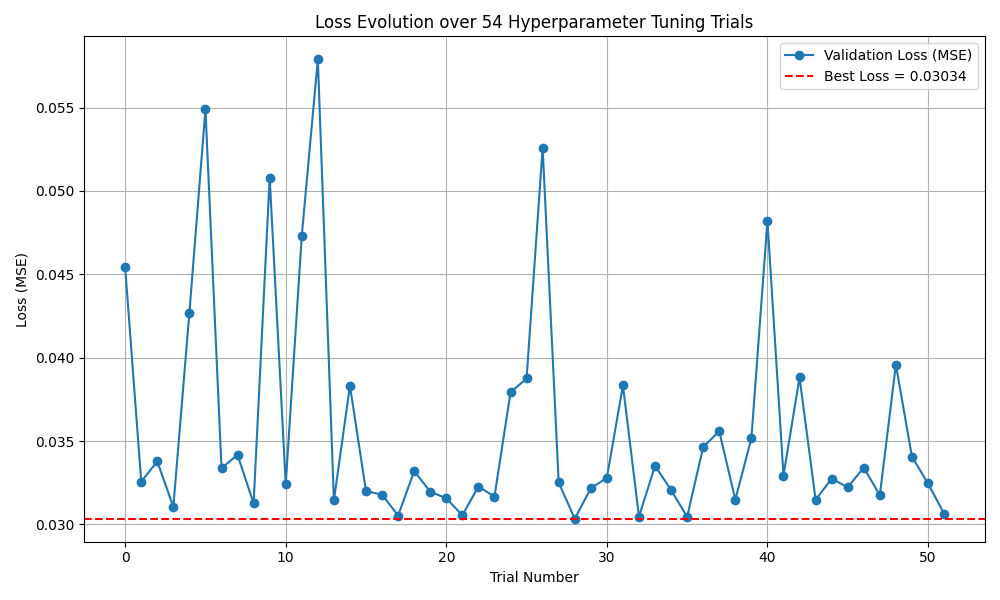
\includegraphics[width=1\linewidth]{loss_hyperparameters.png}
    \caption{Visual representation of the loss function over trials in hyperparameter tuning}
    \label{fig:loss_hyperparameter}
\end{figure}

Figure \ref{fig:loss_hyperparameter} illustrates the evolution of the validation MSE over all tuning trials.
Several other trials achieved losses close to the best-achieving one (e.g. trial 18).
These well-performing trials shared nearly identical architectures, differing in learning rate. 
This consistency supports the robustness of the design. 



\subsection{Results after hyperparameter training}
After hyperparameter tuning, the model was runned again. Hereby, the parameters of section 7.2 were used.
As in the part of the first results, the images of the training mice can be found in this section.
Figure \ref{fig:second_sagittal}, Figure \ref{fig:second_transax} and Figure \ref{fig:second_coronal} represent the different planes.
Images of the test mice can be found in Appendix \ref{Appendix: results after tuning}.
The same division of mice was used, as in indicated in Table \ref{tab:mouse_distribution}.

\begin{figure*}
    \centering
    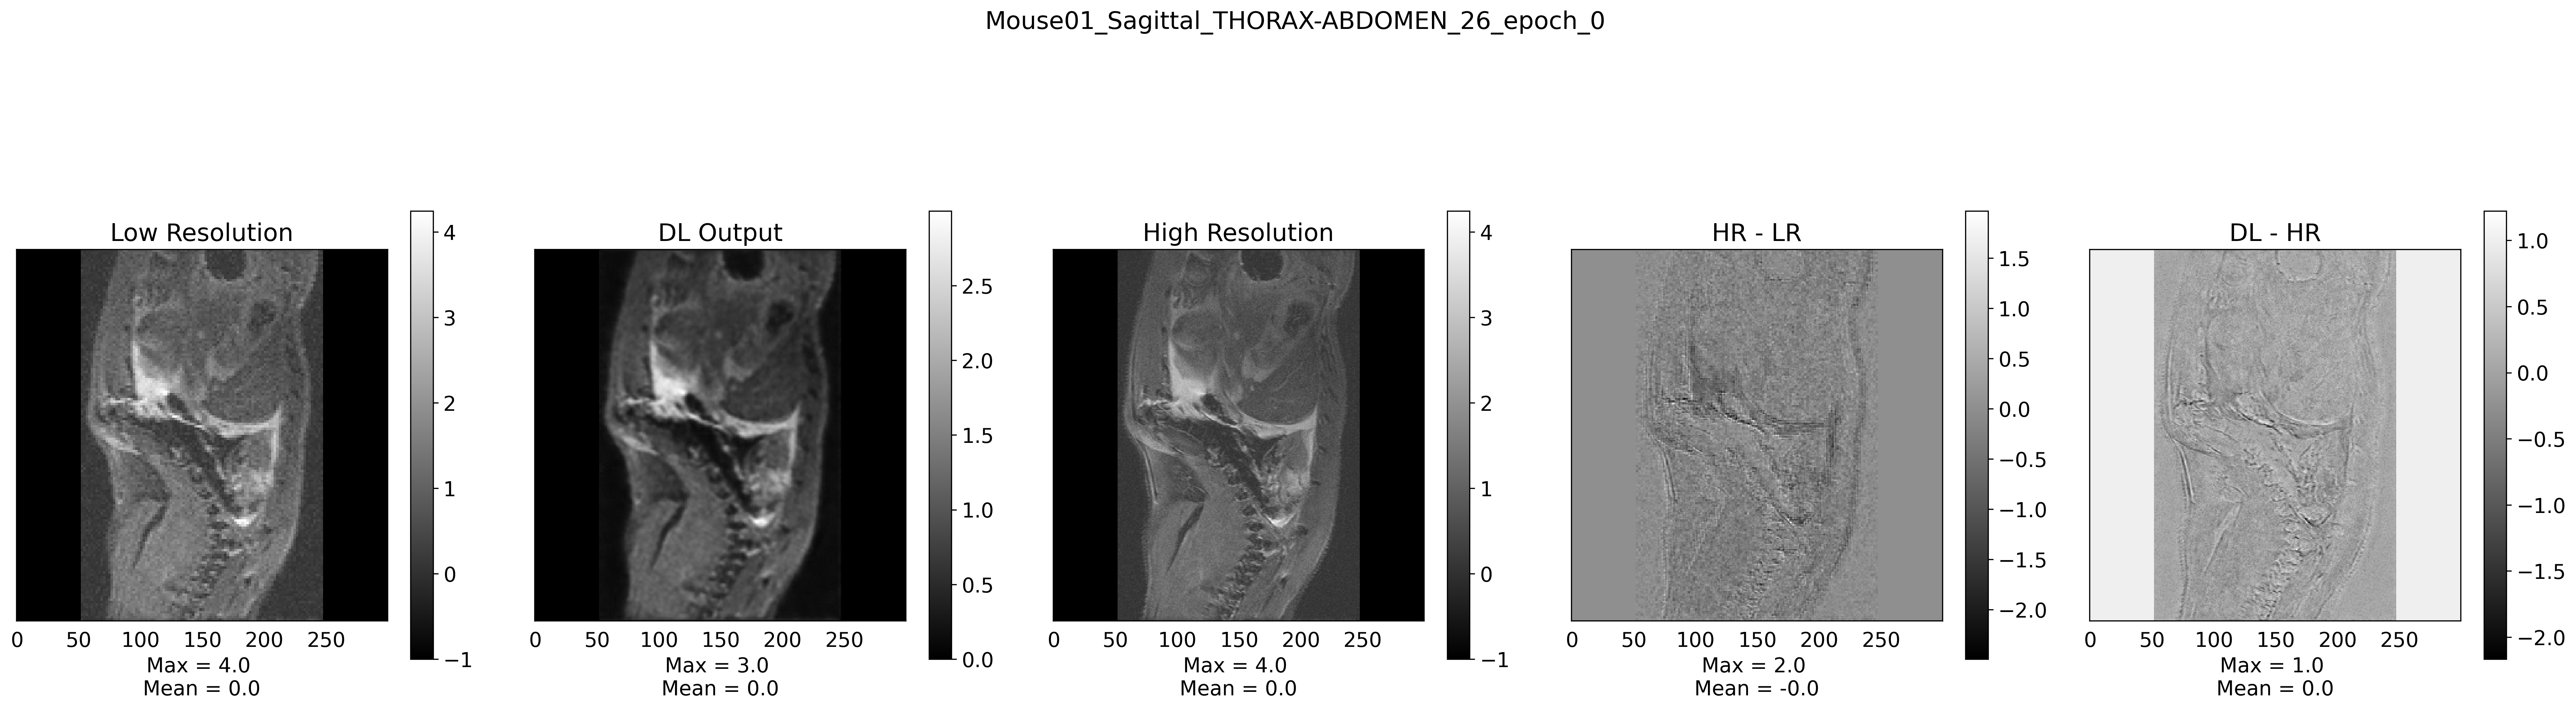
\includegraphics[width=1\linewidth]{Mouse01_Sagittal_THORAX-ABDOMEN_26_epoch_0.png}
    \caption{Results after hyperparameter tuning of abdomen of training mouse.}
    \label{fig:second_sagittal}
\end{figure*}

\begin{figure*}
    \centering
    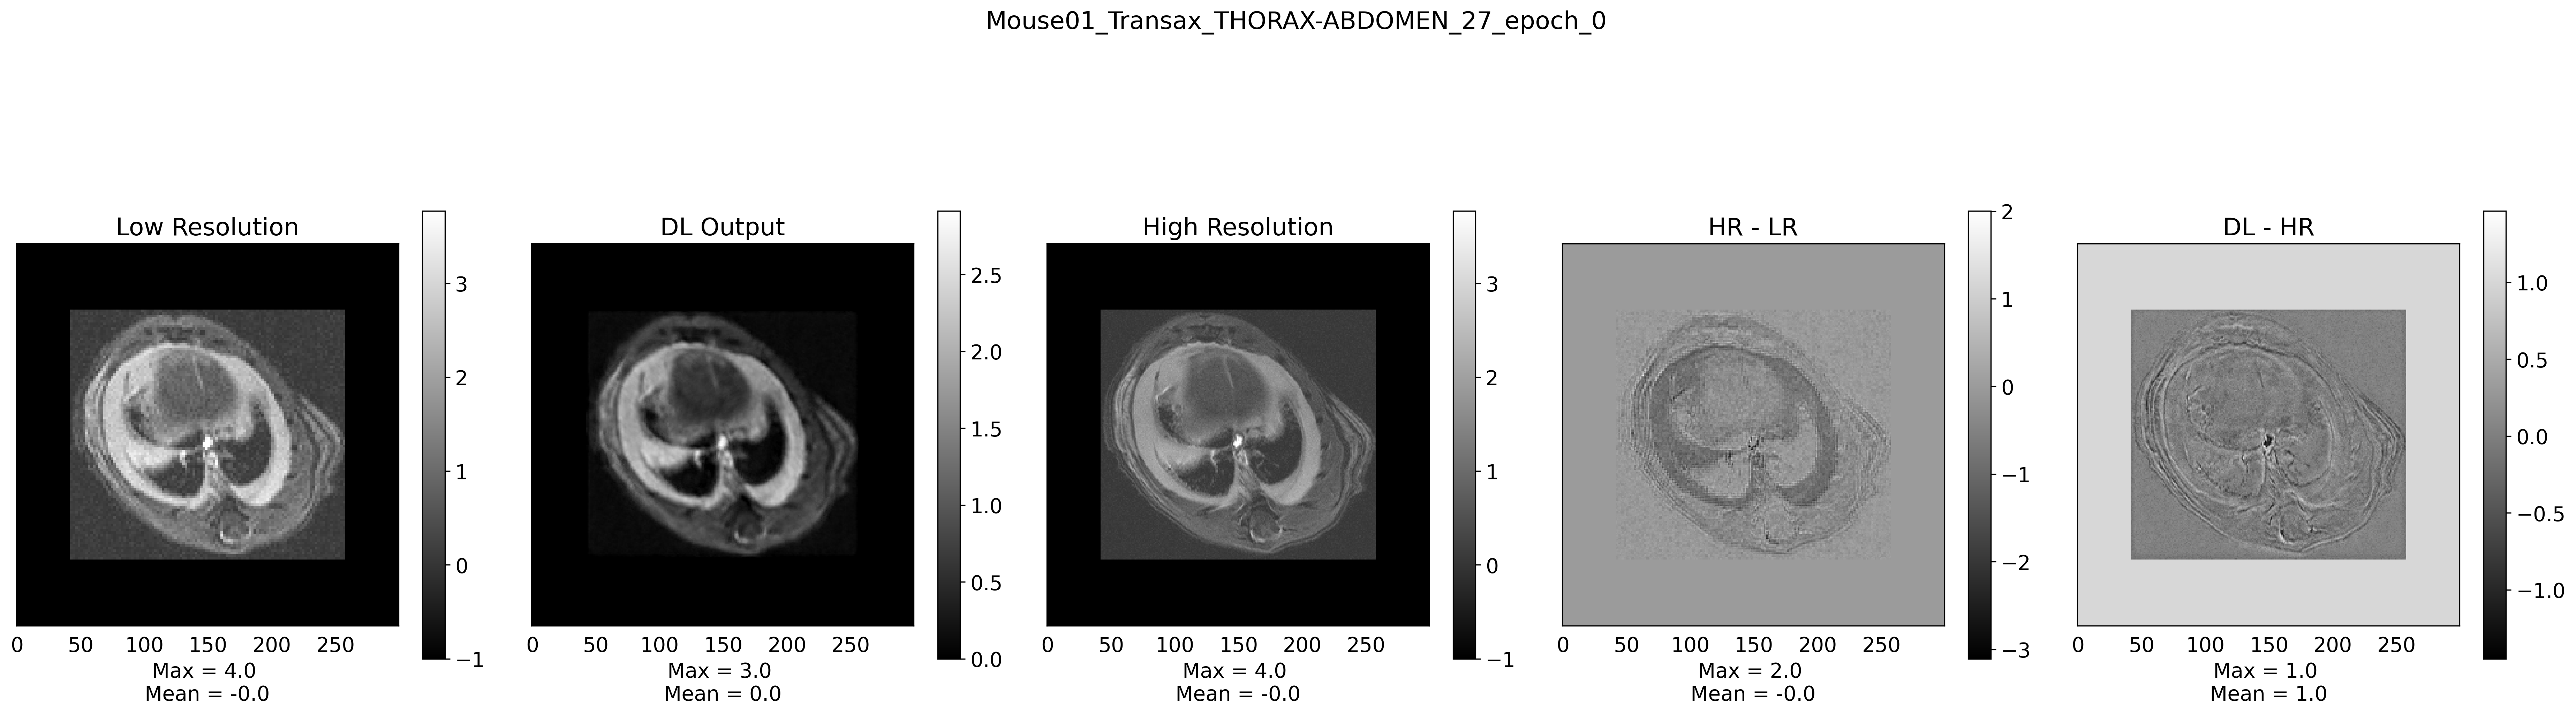
\includegraphics[width=1\linewidth]{Mouse01_Transax_THORAX-ABDOMEN_27_epoch_0.png}
    \caption{Results after hyperparameter tuning of abdomen of training mouse.}
    \label{fig:second_transax}
\end{figure*}

\begin{figure*}
    \centering
    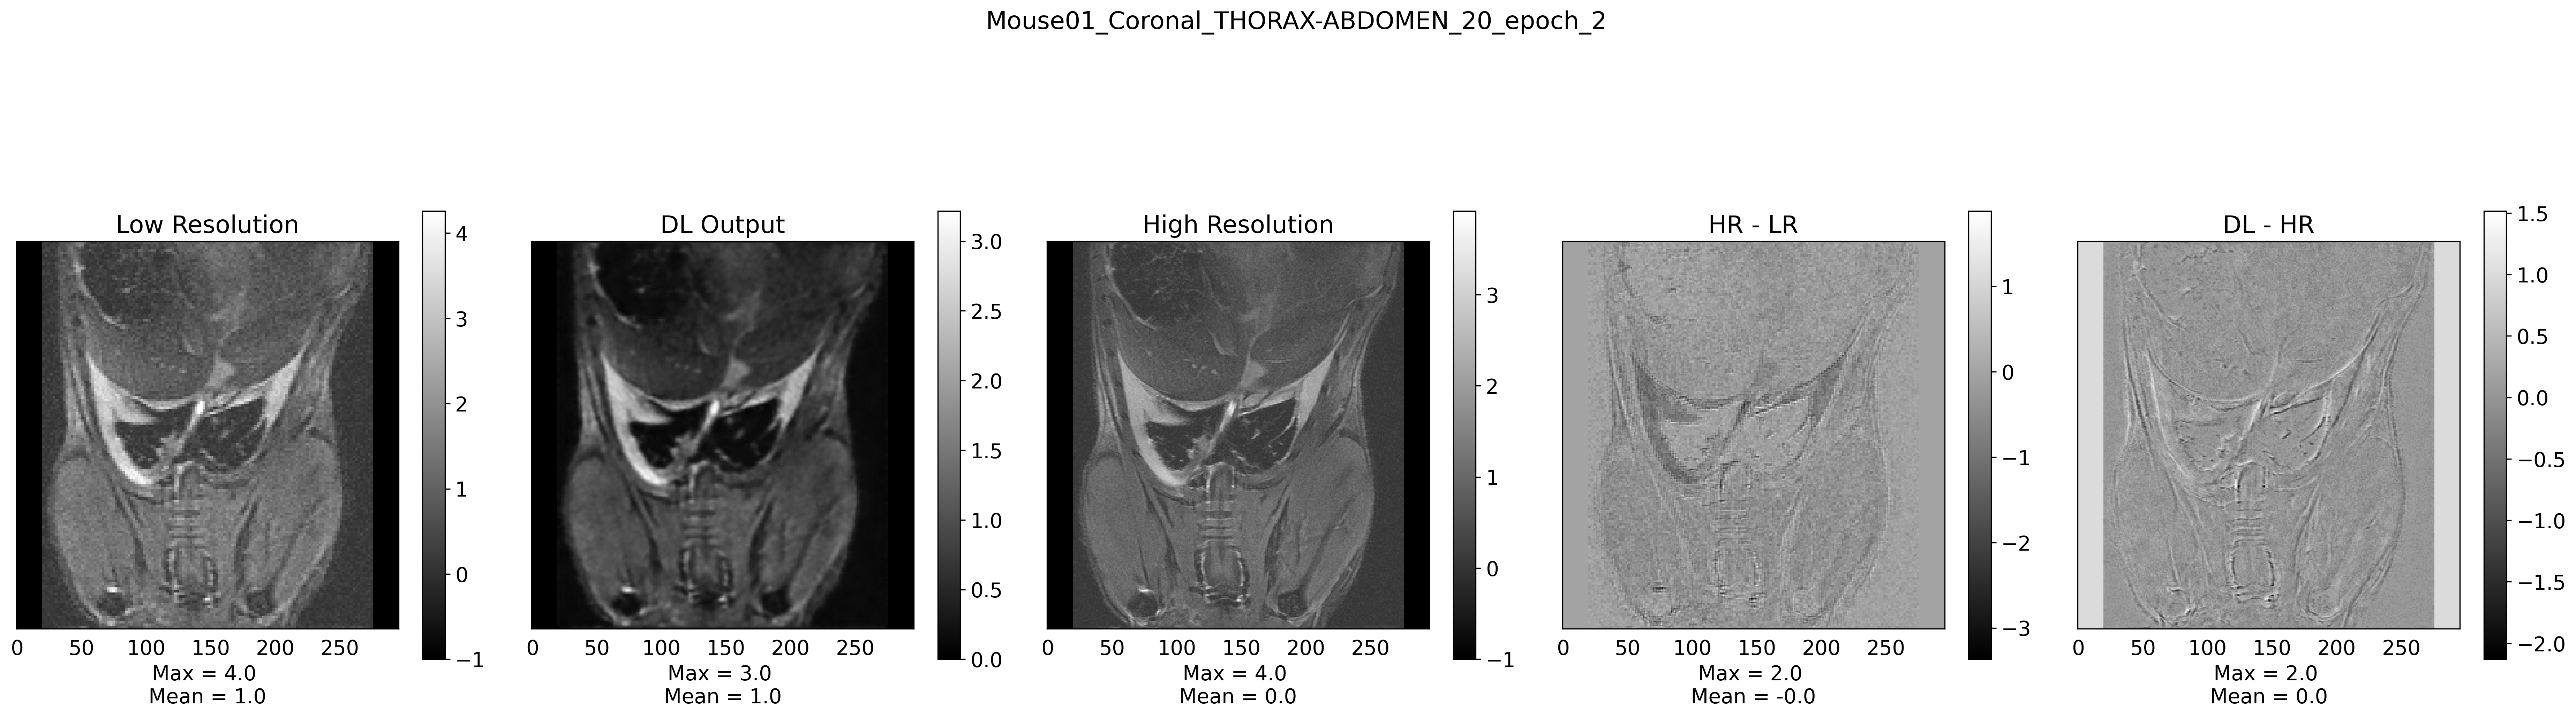
\includegraphics[width=1\linewidth]{Mouse01_Coronal_THORAX-ABDOMEN_20_epoch_2.png}
    \caption{Results after hyperparameter tuning of abdomen of training mouse.}
    \label{fig:second_coronal}
\end{figure*}
   

\subsection{APDDM}

\subsection{Validation}


\subsubsection{Visual comparison}
Figure \ref{fig:val_1} shows a sagittal view of the mouse spine and surrounding anatomy. 
The yellow box highlights the lower thoracic to lumbar spine, an area where fine bone structure is particularly important. 
The LR input of the spine and organ boundaries is quite noisy. 
The DL output is somewhat sharper for example, the white spine column and rib edges within the yellow-highlighted region are brighter and better defined than in LR. 
However, the DL image still lacks the crisp detail of the HR reference. 
Subtle textures, especially within and around the spine, are smoothed out.

\begin{figure*}
    \centering
    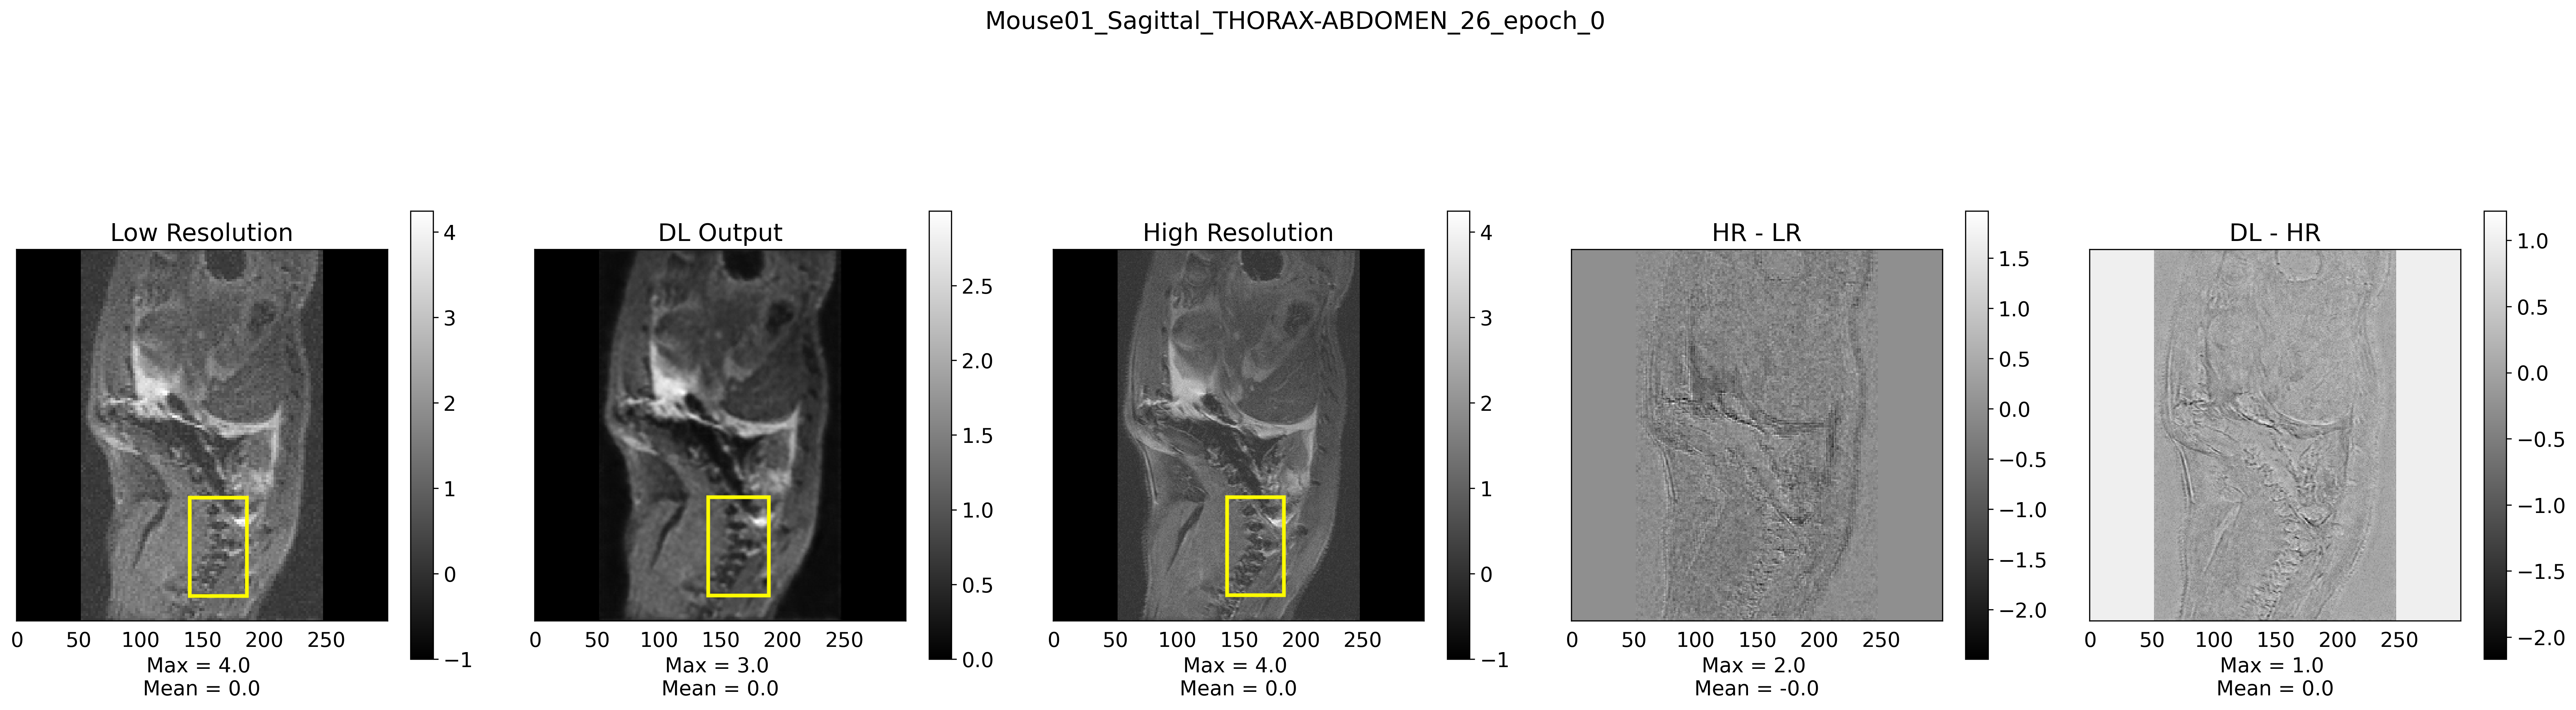
\includegraphics[width=1\linewidth]{Mouse01_Sagittal_val.png}
    \caption{Sagittal view of the mouse thorax-abdomen region (Mouse01)}
    \label{fig:val_1}
\end{figure*}


In Figure \ref{fig:val_2} the yellow arrow is pointing to the lung cavity, where the deep learning output preserves some fine internal structures,
that are obscured by noise in the LR image. This demonstrates that the DL model can retain anatomical detail in high contrast regions. 
The green circle on the other hand highlights a region where the noisiness in the LR image is replaced by blurring in the DL output. 
While the DL network successfully suppresses random noise, it also removes some potential subtle textures, which can be seen in the HR image. 
This is distinct from the classic oversmoothing, as in this case the input itself lacks clear structure. 
This does show the tendency of the model to flatten areas instead of attempting high-frequency recovery.
The residual maps further emphasize these differences.

\begin{figure*}
    \centering
    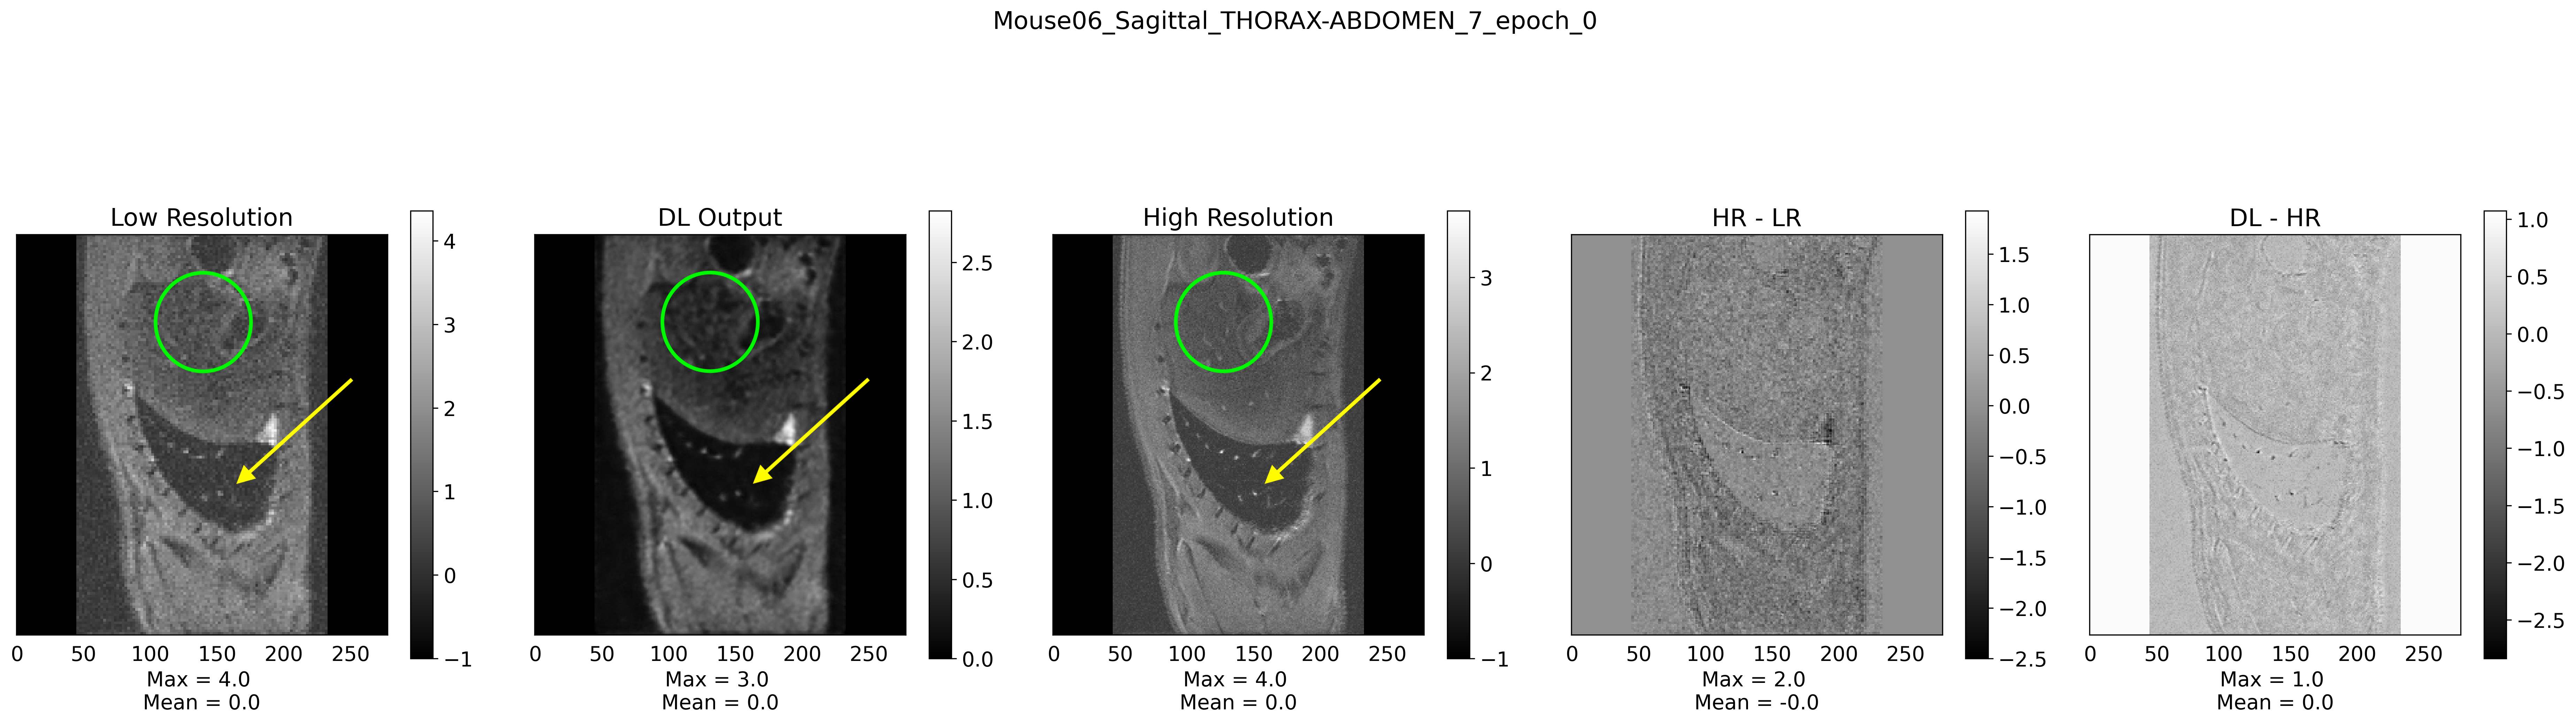
\includegraphics[width=1\linewidth]{Mouse06_Sagittal_val.png}
    \caption{Sagittal view of the mouse thorax-abdomen region (Mouse06)}
    \label{fig:val_2}
\end{figure*}

Figure \ref{fig:val_3} shows the spinal column (bright vertebrae, highlighted by the yellow rectangle), with abdomen  above (highlighted by the green circle). 
In the LR image, the green-circled region is dominated by noise, making it hard to distinguish anatomical content from background variation. 
In the DL output, this area shows reduced noise, which improves the visibility of the underlying structures, though fine detail remains limited. 
DL gains some clarity over LR, especially around the vertebral column (yellow rectangle), but this improvement is still modest. 
The vertebral outlines are only faintly improved. In the HR-LR difference map, the vertebral bone and joint edges stand out strongly, reflecting the detail missing in LR. 
The DL-HR residual still traces those same locations, though with reduced amplitude, indicating partial recovery of anatomical edges. 
This pattern is evident throughout both highlighted areas: the network removes large-scale blur and suppresses noise but leaves behind residual contours at anatomical edges. 
Overall, DL improves global sharpness and interpretability over LR, especially in noisy regions like the top soft tissue (green circle), but continues to blur finer anatomical features.

\begin{figure*}
    \centering
    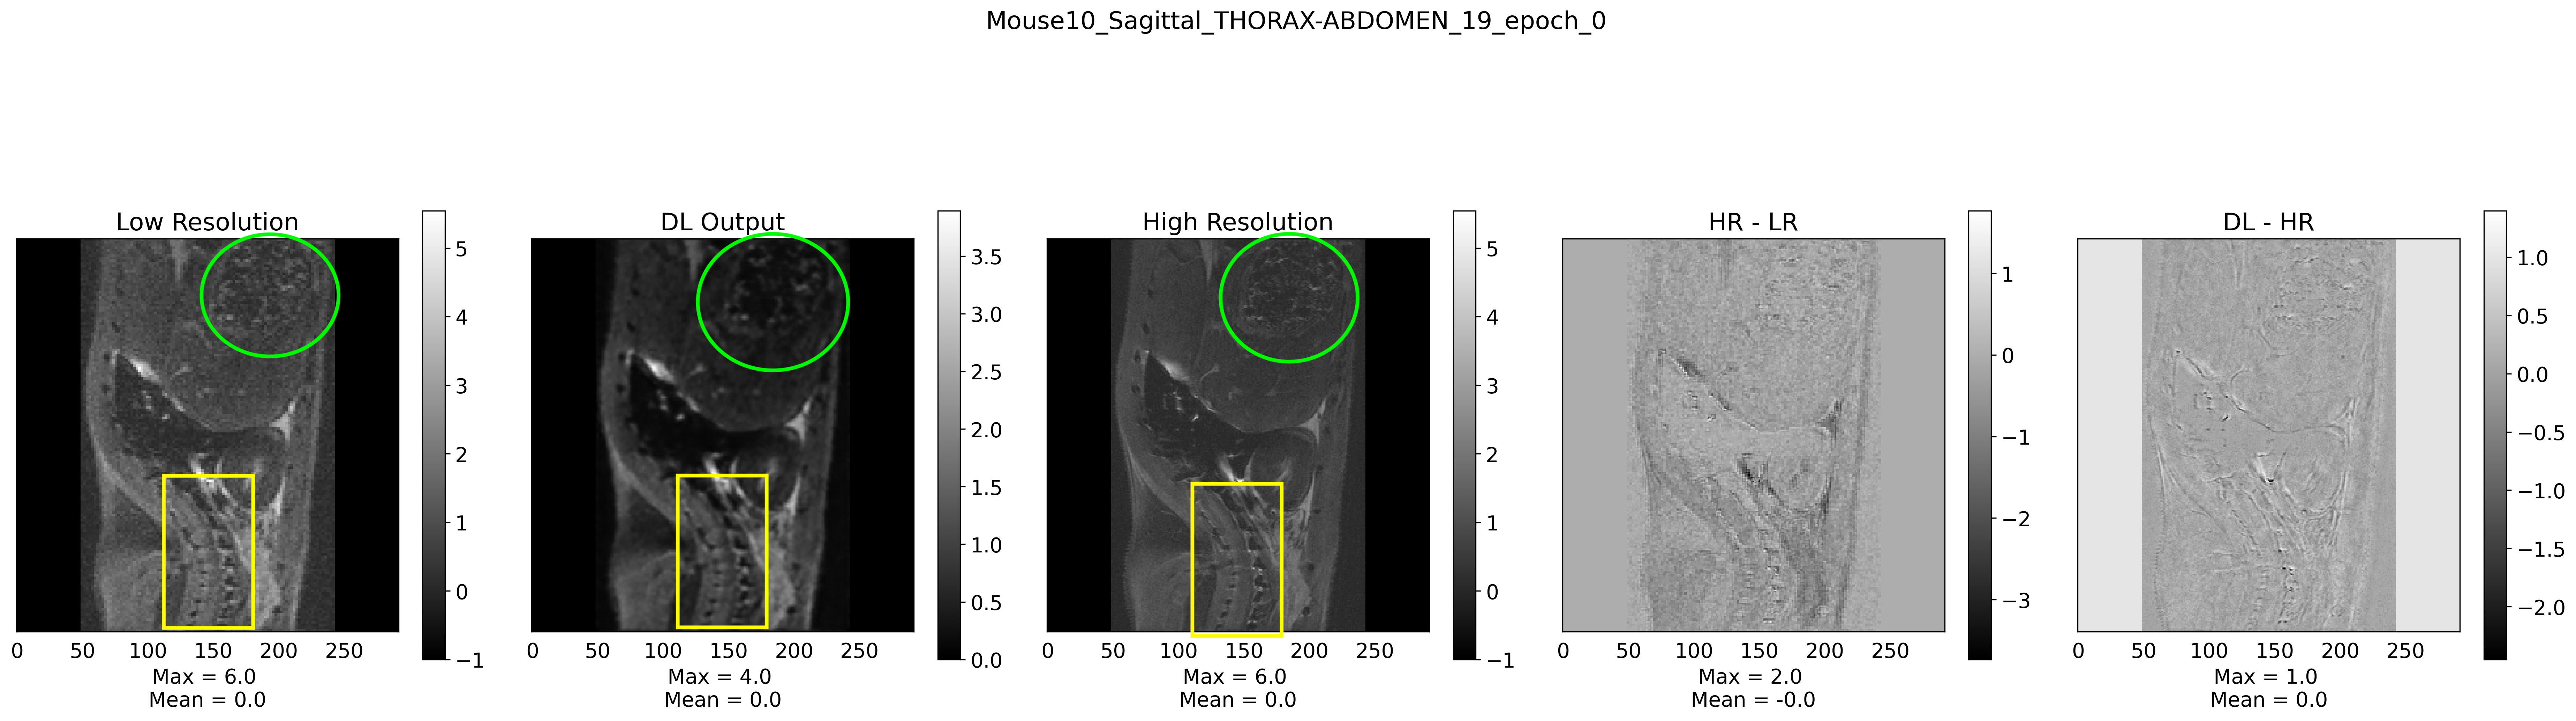
\includegraphics[width=1\linewidth]{Mouse10_Sagittal_val.png}
    \caption{Sagittal view of the spine and pelvic region (Mouse10).}
    \label{fig:val_3}
\end{figure*}



\subsubsection{MSE and SSIM}
Table \ref{tab:MSE_SSIM}  shows the obtained values for MSE and SSIM. The SSIM values range from 0.138 to 0.666, and the MSE values range from 0.001 to 0.055.

\begin{table*}[h!]
    \centering
    \caption{\label{tab:MSE_SSIM} MSE and SSIM values.}
    \resizebox{0.8\linewidth}{!}{
    \begin{tabular}{l|c|c|c|c|c|c}
    \toprule
     & \textbf{Mouse} & \textbf{Plane} & \textbf{Slice} & \textbf{Region} & \textbf{MSE} & \textbf{SSIM} \\
    \midrule
     & 1     & Coronal     & 10    & TA    & 0.007 & 0.575 \\
     &  & Sagittal    & 6     & TA    & 0.003 & 0.484 \\
     &  & Transax     & 13    & TA    & 0.004 & 0.546 \\
    \midrule
     & 6     & Coronal     & 7     & TA    & 0.012 & 0.499 \\
     &  & Sagittal    & 10    & TA    & 0.018 & 0.238 \\
     &  & Transax     & 21    & HT    & 0.012 & 0.564 \\
    \midrule
     & 7     & Coronal     & 11    & TA    & 0.018 & 0.288 \\
     &  & Sagittal    & 11    & TA    & 0.055 & 0.138 \\
     &  & Transax     & 12    & TA    & 0.020 & 0.254 \\
    \midrule
     & 10    & Coronal     & 5     & TA    & 0.006 & 0.592 \\
     &  & Sagittal    & 11    & TA    & 0.003 & 0.551 \\
     &  & Transax     & 22    & HT    & 0.007 & 0.620 \\
    \midrule
     & 23    & Coronal     & 22    & HT    & 0.019 & 0.534 \\
     &  & Sagittal    & 10    & TA    & 0.002 & 0.658 \\
     &  & Transax     & 4     & TA    & 0.001 & 0.666 \\
    \bottomrule
    \end{tabular}
    }
\end{table*}




\subsubsection{Contrast-to-noise ratio}
The obtained values values of Amide were inserted in Equation \ref{eq:CNR} and Equation \ref{eq:normsigma}.
The final values for the CNR are represented in Table \ref{tab:CNR} and the normalised variation values are shown in Table \ref{tab:norm_var}.

\begin{table*}[h!]
    \centering
    \caption{\label{tab:CNR} Overview of the mice, slices and planes used to obtain CNR in LR, DL and HR images. TA stands for thorax-abdomen, while HT is used for head-thorax.}
    \resizebox{0.8\linewidth}{!}{
    \begin{tabular}{l|c|c|c|c|c|c|c}
    \toprule
     & \textbf{Mouse} & \textbf{Plane} & \textbf{Slice} & \textbf{Region} & \textbf{LR CNR} & \textbf{DL CNR} & \textbf{HR CNR} \\
    \midrule
     & 1  & Sagittal   & 6             &TA              &7.365                 & 31.441                & 6.616                  \\
     &    & Transaxial & 13             &TA              & -155.242                &  -706.785               &   -270.741               \\
     &    & Coronal    & 10            &TA              &   -14,699              &    -426.689             &        -179.984           \\

    \midrule
     & 6 & Sagittal    & 10            &TA              &  3.530               &     31.358            &     3.609              \\
     &    & Transaxial   & 21             &HT              &  8.591               &   32.692              &       7.453            \\
     &    & Coronal    & 7            &TA              &  -3.783               &     -10.655            &              -4.075     \\

    \midrule
     & 22 & Sagittal & 12            &HT              &     -8.5587            &      -5.628           &     -10.207              \\
     &    & Transaxial & 8            &TA              &       -3.057          &     -9.234            &      -2.971             \\
     &    & Coronal & 13            &TA              &        -4.414         &      -7.264           &          -4.101         \\
     \bottomrule
    \end{tabular}
    }
\end{table*}

\begin{table*}[h!]
    \centering
    \caption{\label{tab:norm_var} Overview of the mice, slices and planes used to obtain normalised variance in LR, DL and HR images. TA stands for thorax-abdomen, while HT is used for head-thorax.}
    \resizebox{0.8\linewidth}{!}{
    \begin{tabular}{l|c|c|c|c|c|c|c}
    \toprule
     & \textbf{Mouse} & \textbf{Plane} & \textbf{Slice} & \textbf{Region} & \textbf{LR normalised variance} & \textbf{DL normalised variance} & \textbf{HR normalised variance} \\
    \midrule
     & 1  & Sagittal   & 6             &TA              &0.571                 &0.112                 &0.558                   \\
     &    & Transaxial & 13             &TA              &0.005                 &0.001                 &0.003                   \\
     &    & Coronal    & 10            &TA              &0.051                 &0.002                &0.004                   \\
    \midrule
     & 23 & Sagittal    & 10            &TA              &0.099                 &0.095                 &0.057                   \\
     &    & Transaxial   & 4             &TA              &0.091                 &0.081                 &0.130                   \\
     &    & Coronal    & 22            &HT              &0.153                 &0.800               &0.134                   \\
    \midrule
     & 6 & Sagittal    & 10            &TA              &0.449                 &0.102                 &0.657                   \\
     &    & Transaxial   & 21             &HT              &0.119                 &0.040                 &0.157                   \\
     &    & Coronal    & 7            &TA              &0.188                 &0.067                 &0.180                   \\
    \midrule
     & 10 & Sagittal & 11            &TA              &0.273                 &0.0164                 &0.260                   \\
     &    & Transaxial & 22            &HT              &0.045                 &0.032                 &0.067                   \\
     &    & Coronal & 5            &TA              &0.097                 &0.071                 &0.115                   \\
    \midrule
     & 7  & Sagittal & 11            &TA              &0.259                 &0.132                 &0.263                   \\
     &    & Transaxial & 12            &TA              &0.170                &0.082                 &0.175                   \\
     &    & Coronal & 11            &TA              &0.288               &0.123                 &0.228                   \\
    \midrule
     & 22 & Sagittal & 12            &HT              &0.107                 &0.090                 &0.090                   \\
     &    & Transaxial & 8            &TA              &0.190                 &0.151                 &0.190                   \\
     &    & Coronal & 13            &TA              &0.187                 &0.113                 &0.188                   \\
     \bottomrule
    \end{tabular}
    }
\end{table*}

\subsubsection{LEGO phantom test}
For extra validation the model was tested on a 1 min scan of a LEGO brick and compared to its 12 min scan target. The results can be seen in Figure \ref{fig:lego_phantom_test}.
The DL output has suppressed some echo artifacts that are present in the LR image between the black pins. The residuals show that the sharper edges and rectangular shapes are closer to the HR image in the LR image.

\section{Discussion}
\subsection{First results}
After obtaining the first results, a visual validation was made. At first sight, the results were very promising. 
Figure \ref{fig:first_sagittal}, Figure \ref{fig:first_transax} and Figure \ref{fig:first_coronal} shows that the deep learning (DL) image has clearly higher quality and sharper details compared to the low resolution (LR) image at the left side. 
The DL image approaches the high resolution (HR), but still has noise and structures that are not totally visible. 
%add picture with arrow indication of this 
Also, some parts are depicted more black than in the HR.
The maximum intensity of the DL image is always lower than the one of the HR and the one of the LR. 
This indicates small intensity bias or scaling difference. This is also due to the background that is cropped in the original images but depicted at the edges and not depicted in the DL output. 
Looking at the edges of the mice in the DL images, it shows that these are generally more smeared out and less sharp than in the HR images. 
The noise of the LR is reduced with minimal loss of important structural information. 
The same observations can be made when looking at the validation mice (see Appendix \ref{Appendix: first results}).
As said, the results are very promising but there is also room for improvement. The first step in this process is training the hyperparameters. 

\subsection{Trained hyperparameters}
The results of the hyperparameter optimization provide insights into the performance of the model. 
Several key hyperparameter choices reflect current best practices in deep learning formedical image restoration, while others diverge in notable ways

The feature dimensions were set to 128, 128, 64, showing that the moderately deep but not excessively wide netwroks achieved optimal performance. 
This allows the network to capture a sufficientrange of spatial features while avoiding overfitting, which is a risk in smaller-scale datasets such as micro-MRI.

Strided convolution (convStrided) was preferred over pooling for downsampling. 
This aligns with expectations from common CNN practive. 
Strided convolution allows the model to practive how to compress feature maps instead of relying on fixed operations such as meanpooling. 
This learnability likely helped preserve critical structural details \cite{springenberg2014}.
For upsampling, bilinear interpolation was favored over learned transposed convolutions. 
Unlike transposed conolutions, which introduce additional parameters and are prone to artifacts, bilinear upsampling provides a smooth and stable to restore spatial dimensions. 
This upsampling method does not learn to add high-frequency details \cite{kolarik2019}.
The consistent selection of bilinear upsampling in high-performing trials suggests that its simplicity and robustness were well-suited for this task.
 
Residual connections were disabled which is an unexpected result which contrasts with many image restoration models that benefit from residual learning. 
In this case the low-resolution and high-resolution images were relatively similar in structure and intensity, making transformations less complex.
This reduces the benefit of residual modeling. 
The U-Net's skip connections inherently serve a similar role to residuals, which likely compensated for this. 
This allows effective feature reuse and reduces the need for a global residual link \cite{xu2024}.

The learning rate was consistently selected in the lower range, supporting gradual and stable learning. 
The chosen scheduler, step learning rate, reduces the learning rate at fixed intervals. 
This allows the network to learn quickly during early eoichs and refine weights more delicately later in training. 
This balance is preferred for restoring subtle textures in high-resolution data. 

Certain parameters were fixed prior to tuning, based on theoretical justification and preliminary experiments. 
The activation function was set to ReLU, chosen over alternatives such as LeakyReLU, PReLU, or ELU. 
Although ReLU is susceptible to the "dying neuron" problem, it remains a robust default in convolutional architectures due to its simplicity, computational efficiency, and effective gradient propagation. 
Initial exploratory tests showed no instability or gradient vanishing that would necessitate more complex activations. 
The network’s stable convergence confirmed that ReLU was a suitable choice for this task.

The loss function was fixed as mean squared error (MSE), a standard objective for pixel-wise regression tasks. 
MSE offers a simple, differentiable, and interpretable loss landscape that aligns well with the goal of minimizing reconstruction error. 
While alternative loss functions, such as SSIM or perceptual loss, were considered, MSE was retained due to its stability and its compatibility with the validation metric used during tuning. 

The optimization process solely relied on MSE for validation.   
This decision may introduce some form of metric bias. 
MSE disproportionately penalizes large pixel errors, which often lead to overly smooth outputs. 
In denoising tasks, this can result in models that reduce noise effectively in terms of pixel accuracy but at the cost of signal preservation, leading to a lower signal-to-noise (SNR) in practice. 
MSE is also sensitive to outliers and intensity shifts, while being oblivious to perceptual structure and contrast consistency \cite{1284395}. 
Future work could benefit from using alternative validation metrics, such as SNR or perceptual similarity measures, to better guide model selection and ensure outputs are both quantitatively accurate and visually informative \cite{chavhan2009t2star}. 
Metrics such as LPIPS (Learned Perceptual Image Patch Similarity) offer a promising alternative by leveraging deep features that align more closely with human perception and quality \cite{zhang2018unreasonableeffectivenessdeepfeatures}.

\subsection{Results after hyperparameter training}
When looking at the results after hyperparameter, it can be seen that the model is still working quite good. 
The DL image in Figure \ref{fig:second_sagittal}, Figure \ref{fig:second_transax} and Figure \ref{fig:second_coronal} shows again sharper details and higher quality compared to the LR image.
The DL image is still more black than the HR image.
The maximum intensity of the DL image is again lower than the ones of the LR and HR image, but the difference is only $1$. 
In the first results, this difference was much higher.
This means the intensity bias and scaling difference are better than previously.
The background also needs to be taken into account, which can also leads to other maximum intensities.
Compared to Figure \ref{fig:first_sagittal}, Figure \ref{fig:first_transax} and Figure \ref{fig:first_coronal}, the images after hyperparameter tuning have sharper edges.
The edges are less smeared out and a bit sharper.
The loss of structural information is still present, but less than previously. 

\subsection{APDDM}

\subsection{Validation}

\subsubsection{Visual comparison}
In all cases the DL output appears to be smoother than the HR reference. This over-smoothing is a known effect of using MSE loss. 
This is due to the network learning to average high-frequency patterns which results on blurred textures. 
The residuals of DL-HR consistently have lower amplitudes than the HR-LR, this means the network shrinks the differences but is unable to restore all fine details \cite{MSE}. 
MSE encourages finding pixel-wise averages of solutions, producing overly-smooth results. Our visual inspection confirms this.

\subsubsection{MSE and SSIM}
High SSIM values in Mouse 23, Transax slice 4 demonstrate accurate preservation of simpler structures. The lower SSIM in Mouse 7, Sagittal slice 11, however, suggests difficulty in accurately reconstructing its more complex anatomical details. The overall low MSE values, imply that the overall pixel intensity is preserved well in the deep learning reconstruction.  
These MSE values together with the varying SSIM values, suggests that while the network correctly preserves the general appearance, the accuracy of fine anatomical details varies. Further investigation into the specific anatomical features present in the slices with lower SSIM could be a guide for how the model can be improved.

\subsubsection{Contrast-to-noise ratio}
First, the CNR was examined across the different image types. When comparing absolute values the DL\_CNR is consistenlty the highest but no consistent pattern can be observed between the LR\_CNR and HR\_CNR. 
This variability can be attributed to several factors. First, MRI is not a quantitive imagining technique. Pixel intensity values are relative rather than standardized. There is a certain maximum pixel value, which is influenced by acquisition parameters, reconstruction algorithms and normalization steps.
A key factor affecting the CNR is the dynamic range of the image. Dynamic range refers to the difference between the minimum and maximum intensity values in an image.
The LR image contains more noise, which means the pixel values are more similar. This directly affects the dynamic range because the difference between minimum and maximum intensity values becomes smaller, resulting in a lower CNR.
On the other hand, a HR image has less noise, which means the difference between minimum and maximum intensity will be higher. This leads to a higher dynamic range and, consequently, a higher CNR. 
Furthermore, interpolation is done, which results in a smoothing. This smoothing alters the intensity distribution and direclty implies CNR.

After these observations were made, the normalized variation was also evaluated. As shown in Table \ref{tab:norm_var}, a clear and consistent pattern emerges: the DL-normalized variation is consistently the lowest across all cases, while the LR-normalized variation is consistently the highest.
This trend can be attributed to the behavior of the deep learning model, which is trained to reduce the noise while preserving structural information. As a result, the standard deviation of the background region is significantly reduced, while the mean background intensity remains relatively stable.
This leads to lower normalized variation values for DL images, which is indicative of improved image quality and less noise.
Conversely, the LR image exhibit higher normalized variation due to increased noise levels. In these images, the mean of the background is generally higher.
A detailed overview is given in Appendix \ref{Appendix: val}.


\subsubsection{LEGO brick phantom}
As an extra validation step, an MRI scan of a LEGO brick with a 1-minute scan time was given as input to the trained model and compared with its 12-minute scan time counterpart. This can show whether the model is overtrained and whether it could potentially be used to denoise and improve shorter scan time images of objects other than mice. The images discussed here can be seen in Figure \ref{fig:lego_phantom_test}.

Visually, the model produces an output that strongly resembles both the LR and HR images. The model removes noise in the grey regions from the LR image, as well as echo artifacts that can be seen, for example, between the black LEGO pins at the top. The rectangular shapes are preserved, although the training data of mice did not contain many such shapes.

However, comparing the residuals shows that the LR image is closer to the HR image in terms of the rectangles than the DL image. This could be due to the fact that the model was trained on mouse scans, which, as mentioned, do not contain the sharp edges characteristic of a LEGO brick, and that the model used MSE as the loss function during training. MSE penalizes large pixel errors, so the model tends to smooth out sharp changes.

The MSE between the DL and HR images is 0.1269, and between the LR and HR images is 0.0737 (an increase of 72\% from the LR to the DL image). This means that if we only consider the pixel-wise error, the LR image remains a better approximation of the HR image than the DL image.

Another indicator of image quality is the Structural Similarity Index Measure (SSIM), as discussed in section \ref{Structural similarity index measure}. The DL and HR images have an SSIM of 0.4548, while the LR and HR images have one of 0.4624. So the SSIMs differ by only 1.6\%, indicating that according to SSIM, neither the LR nor the DL image is clearly a better approximation of the HR image. Very similar conclusions regarding MSE and SSIM can be drawn from examining other slices of the LEGO phantom.

It is important to note that MSE and SSIM are purely quantitative metrics and should be considered as supplementary to qualitative visual assessment. Despite the DL image having a slightly higher MSE and lower SSIM than the LR image, it remains a strong approximation of the HR image due to its effective denoising and artifact suppression capabilities, also for objects different from mice.




\begin{figure*}
    \centering
    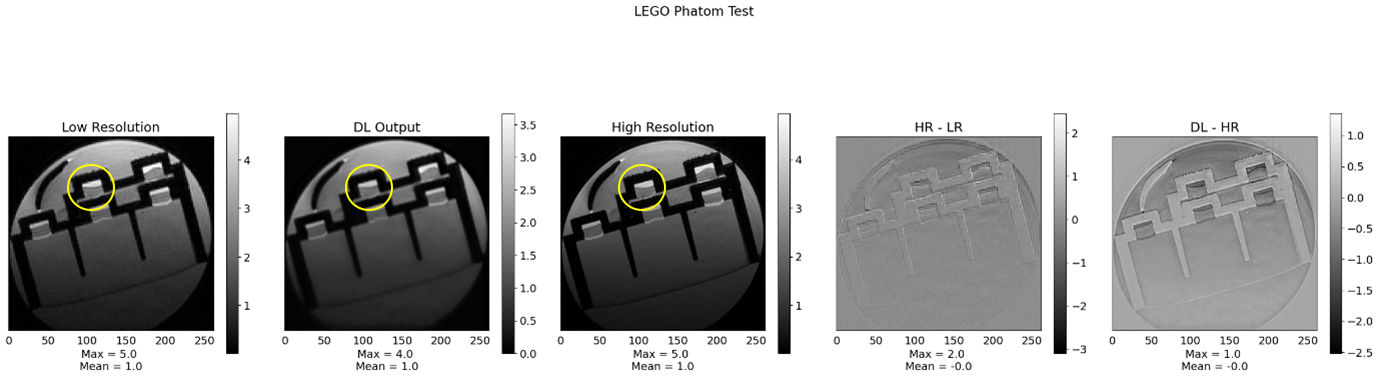
\includegraphics[width=1\linewidth]{LEGO_phantom_test.png}
    \caption{Results after hyperparameter tuning of LEGO phantom.}
    \label{fig:lego_phantom_test}
\end{figure*}





\section{Conclusion}

Both the U-Net and APDDM deep learning methods improved image quality of LR images. The main improvement is the denoising, however fine details may still get lost due to an 'oversmoothing' effect that is attirbuted to the use of the MSE as loss function, which penalizes pixel-wise errors. And as could be concluded from the LEGO phantom quality control, orthogonal borders and shapes are better preserved in the LR image than in the DL image.
Furthermore, it wwas demonstrated that the APDDM outperformed the U-Net.


\newpage
\onecolumn
\nocite{*}
\begin{thebibliography}{99}

    \bibitem{brown2014magnetic} Brown, R. W., Cheng, Y.-C. N., Haacke, E. M., Thompson, M. R., \& Venkatesan, R. (2014). \textit{Magnetic Resonance Imaging: Physical Principles and Sequence Design}. John Wiley \& Sons.
    
    \bibitem{mrimaster2024} Mrimaster. (2024, June). TR and TE in MRI — TR (repetition time), TE (echo time) and image contrast. Retrieved March 25, 2025, from \url{https://mrimaster.com/tr-and-te-in-mri/}.
    
    \bibitem{ronneberger2015unet} Ronneberger, O., Fischer, P., \& Brox, T. (2015). U-/Net: Convolutional Networks for Biomedical Image Segmentation. In \textit{Medical Image Computing and Computer-Assisted Intervention (MICCAI)} (pp. 234–241). Springer. \url{https://doi.org/10.1007/978-3-319-24574-4_28}.
    
    \bibitem{bruker2025pharmascan} Bruker. (2025). PharmaScan — Preclinical MRI. Retrieved March 25, 2025, from \url{https://www.bruker.com/en/products-and-solutions/preclinical-imaging/mri/pharmascan-new.html}.
    
    \bibitem{grover2015mri} Grover, V. P. B., Tognarelli, J. M., Crossey, M. M. E., Cox, I. J., Taylor-Robinson, S. D., \& McPhail, M. J. W. (2015). Magnetic Resonance Imaging: Principles and Techniques: Lessons for Clinicians. \textit{Journal of Clinical and Experimental Hepatology}, 5(3), 246–255. \url{https://doi.org/10.1016/j.jceh.2015.08.001}.
    
    \bibitem{chavhan2009t2star} Chavhan, G. B., Babyn, P. S., Thomas, B., Shroff, M. M., \& Haacke, E. M. (2009). Principles, Techniques, and Applications of T2/*-based MR Imaging and Its Special Applications. \textit{Radiographics}, 29(5), 1433–1449. \url{https://doi.org/10.1148/rg.295095034}.
    
    \bibitem{tran2025unet} Tran, M. (2025, January). Understanding U-/Net. Retrieved March 25, 2025, from \url{https://towardsdatascience.com/understanding-u-net-61276b10f360/}.
    
    \bibitem{verhelst2025denoising} Verhelst, N., Courtens, J., Vervenne, B., Abi Akl, M., Maebe, J., Lajtos, M., Vandenberghe, S., Vanhove, C., \& Muller, F. M. (2025). Deep Learning for Denoising and Super-Resolution in Low-Resolution Micro-MRI for Mouse Imaging: Achieving Shorter Scan Times. In \textit{Proceedings of the 20th European Molecular Imaging Meeting (EMIM)} (p. 1).
    
    \bibitem{10.1145/3292500.3330701} Akiba, T., Sano, S., Yanase, T., Ohta, T., \& Koyama, M. (2019). Optuna: A Next-generation Hyperparameter Optimization Framework. In \textit{Proceedings of the 25th ACM SIGKDD International Conference on Knowledge Discovery \& Data Mining} (pp. 2623–2631). ACM. \url{https://doi.org/10.1145/3292500.3330701}.
    
    \bibitem{unknown-author-no-date} Unknown Author. (n.d.). Tutorials. Retrieved from \url{https://www.overleaf.com/learn/latex/Tutorials}.
    
    \bibitem{massed-compute-2025} Massed Compute. (2025, February). FAQ Answers - Massed compute. Retrieved from \url{https://massedcompute.com/faq-answers/?question=What%20are%20the%20key%20differences%20between%20Adam%20and%20SGD%20optimizers%20in%20large%20language%20model%20training?}.
    
    \bibitem{sanghvirajit-2025} Sanghvirajit. (2025, March). Everything you need to know about Adam and RMSprop Optimizer. Retrieved from \url{https://medium.com/analytics-vidhya/a-complete-guide-to-adam-and-rmsprop-optimizer-75f4502d83be}.
    
    \bibitem{pykes-2021} Pykes, K. (2021, October). AdamW Optimizer in PyTorch Tutorial. Retrieved from \url{https://www.datacamp.com/tutorial/adamw-optimizer-in-pytorch}.
    
    \bibitem{dhanushkumar-2023} DhanushKumar. (2023, November). MAX POOLING - DhanushKumar - Medium. Retrieved from \url{https://medium.com/@danushidk507/max-pooling-ef545993b6e4}.
    
    \bibitem{unknown-author-no-date2} Unknown Author. (n.d.). 7.3. Padding and Stride — Dive into Deep Learning 1.0.3 documentation. Retrieved from \url{https://d2l.ai/chapter_convolutional-neural-networks/padding-and-strides.html}.
    
    \bibitem{isbhargav-2020} Isbhargav. (2020, July). Guide to Pytorch Learning Rate Scheduling. Retrieved from \url{https://www.kaggle.com/code/isbhargav/guide-to-pytorch-learning-rate-scheduling}.
    
    \bibitem{unknown-author-no-date3} Unknown Author. (n.d.). Comprehensive overview of learning rate schedulers in Machine Learning | CloudFactory Computer Vision Wiki. Retrieved from \url{https://wiki.cloudfactory.com/docs/mp-wiki/scheduler}.
    
    \bibitem{unknown-author-2025} Unknown Author. (2025, April). Bicubic Interpolation | CloudInary. Retrieved from \url{https://cloudinary.com/glossary/bicubic-interpolation}.
    
    \bibitem{amanrao-2023} Amanrao. (2023, September). Image Upscaling using Bicubic Interpolation - Amanrao - Medium. Retrieved from \url{https://medium.com/@amanrao032/image-upscaling-using-bicubic-interpolation-ddb37295df0}.
    
    \bibitem{jordan_2018_setting} Jordan, J. (2018, March). Setting the learning rate of your neural network. Retrieved from \url{https://www.jeremyjordan.me/nn-learning-rate/}.
    
    \bibitem{anderson_2023_loss} Anderson, M. (2023, February). Loss Functions in Machine Learning - Metaphysic.ai. Retrieved April 13, 2025, from \url{https://blog.metaphysic.ai/loss-functions-in-machine-learning/}.
    
    \bibitem{DDPM} Ho, J., Jain, A., \& Abbeel, P. (2020). Denoising diffusion probabilistic models. Advances in neural information processing systems, 33, 6840-6851.

    \bibitem{bharatiya_2019_comprehensive} Bharatiya, P. (2019, September). Comprehensive Guide to the ReLU Activation Function in Neural Networks: Definition, Role, and Type Explained. Retrieved from \href{https://data-intelligence.hashnode.dev/comprehensive-guide-to-the-relu-activation-function-in-neural-networks-definition-role-and-type-explained}{https://data-intelligence.hashnode.dev/comprehensive-guide-to-the-relu-activation-function-in-neural-networks-definition-role-and-type-explained}.
    
    \bibitem{mseJim} Frost, J. (2023). Mean Squared Error (MSE). Retrieved April 30, 2025, from \url{https://statisticsbyjim.com/regression/mean-squared-error-mse/}.
    
    \bibitem{dosselmann-2009} Dosselmann, R., \& Yang, X. D. (2009). A comprehensive assessment of the structural similarity index. \textit{Signal Image and Video Processing}, 5(1), 81–91. \url{https://doi.org/10.1007/s11760-009-0144-1}.
    
    \bibitem{9036442} Zaheer, R., \& Shaziya, H. (2019). A Study of the Optimization Algorithms in Deep Learning. In \textit{2019 Third International Conference on Inventive Systems and Control (ICISC)} (pp. 536-539). IEEE. \url{https://doi.org/10.1109/ICISC44355.2019.9036442}.
    
    \bibitem{Dastmalchi} Dastmalchi, H., \& Aghaeinia, H. (2022, June). Super-resolution of very low-resolution face images with a wavelet integrated, identity preserving, adversarial network. \textit{Signal Processing: Image Communication}, 107, 116755. \url{https://doi.org/10.1016/j.image.2022.116755}.
    
    \bibitem{relu} Maniatopoulos, A., \& Mitianoudis, N. (2021). Learnable Leaky ReLU (LeLeLU): An Alternative Accuracy-Optimized Activation Function. \textit{Information}, 12(12), 513. \url{https://www.mdpi.com/2078-2489/12/12/513}.
    
    \bibitem{1284395} Wang, Z., Bovik, A. C., Sheikh, H. R., \& Simoncelli, E. P. (2004). Image quality assessment: from error visibility to structural similarity. \textit{IEEE Transactions on Image Processing}, 13(4), 600–612. \url{https://doi.org/10.1109/TIP.2003.819861}.
    
    \bibitem{zhang2018unreasonableeffectivenessdeepfeatures} Zhang, R., Isola, P., Efros, A. A., Shechtman, E., \& Wang, O. (2018). The Unreasonable Effectiveness of Deep Features as a Perceptual Metric. \textit{arXiv:1801.03924}. Retrieved from \url{https://arxiv.org/abs/1801.03924}.

    \bibitem{springenberg2014} Springenberg, J. T., Dosovitskiy, A., Brox, T., \& Riedmiller, M. (2014). Striving for simplicity: The all convolutional net. \textit{arXiv preprint arXiv:1412.6806}. \url{https://arxiv.org/abs/1412.6806}.
  
    \bibitem{xu2024} Xu, G., Wang, X., Wu, X., Leng, X., \& Xu, Y. (2024). Development of Skip Connection in Deep Neural Networks for Computer Vision and Medical Image Analysis: A Survey. \textit{arXiv preprint arXiv:2405.01725}. \url{https://arxiv.org/abs/2405.01725}

    \bibitem{kolarik2019} Kolařík, M., Burget, R., \& Říha, K. (2019). Upsampling Algorithms for Autoencoder Segmentation Neural Networks: A Comparison Study. \textit{2019 11th International Congress on Ultra Modern Telecommunications and Control Systems and Workshops (ICUMT)}, 1–7. \url{https://ieeexplore.ieee.org/document/8970918}

    \bibitem{MSE} C.~Ledig, L.~Theis, F.~Huszar, J.~Caballero, A.~Cunningham, A.~Acosta, A.~Aitken, A.~Tejani, J.~Totz, Z.~Wang, and W.~Shi, ``Photo-Realistic Single Image Super-Resolution Using a Generative Adversarial Network,'' in \emph{Proceedings of the IEEE Conference on Computer Vision and Pattern Recognition (CVPR)}

    \bibitem{datacamp_optuna} DataCamp, ``Optuna for Deep Reinforcement Learning in Python,'' \textit{DataCamp Tutorials}, Aug. 2024. [Online]. Available: \url{https://www.datacamp.com/tutorial/optuna}.


  \end{thebibliography}

\newpage
\begin{appendices}
\section{Appendix: Gantt chart}
\label{appendix:Division of tasks}

\definecolor{barblue}{RGB}{0,0,128}
\newcommand\RotText[1]{\rotatebox{90}{\parbox{-1cm}{\centering#1}}}

\sffamily
\begin{ganttchart}[
    canvas/.append style={fill=none, draw=black!5, line width=.9pt},
    hgrid style/.style={draw=black!5, line width=.9pt},
    vgrid={*1{draw=black!5, line width=.9pt}},
    title/.style={draw=none, fill=none},
    title label font=\bfseries\footnotesize,
    title label node/.append style={below=7pt},
    include title in canvas=false,
    bar label font=\mdseries\small\color{black!70},
    bar label node/.append style={left=1cm},
    bar/.append style={draw=none, fill=barblue},
    group left shift=0,
    group right shift=0,
    group height=.5,
    group peaks tip position=0,
    group label node/.append style={left=.6cm},
    group progress label font=\bfseries\small,
  ]{1}{13}

  \gantttitle{WEEKS:}{1} \\
  \gantttitlelist{"\RotText{19/2}", "\RotText{26/2}", "\RotText{5/3}", "\RotText{12/3}", "\RotText{19/3}", "\RotText{26/3}", "\RotText{2/4}", "\RotText{9/4}", "\RotText{16/4}", "\RotText{23/4}", "\RotText{30/4}", "\RotText{7/5}", "\RotText{14/5}"}{1} \\

  \ganttbar{Introduction to the project}{1}{1} \\
  \ganttbar{Scanning}{2}{4} \\
  \ganttbar{Intermediate report and presentation}{3}{6} \\
  \ganttbar{Introduction to AI and DL}{4}{6} \\
  \ganttbar{Training hyperparameters}{7}{13} \\
  \ganttbar{Anchored path diffusion}{7}{13} \\
  \ganttbar{Final report}{7}{13}\\
  \ganttbar{Poster}{10}{13}\\
  \ganttbar{Validation}{11}{13}\\
  \ganttbar{Training the model}{12}{12}
  

\end{ganttchart}

\newpage
\section{Appendix: Figures Preprocessing}
\label{Appendix: Figures Preprocessing}

\begin{figure}[h]
    \centering
    \begin{minipage}{0.3\textwidth}
        \centering
        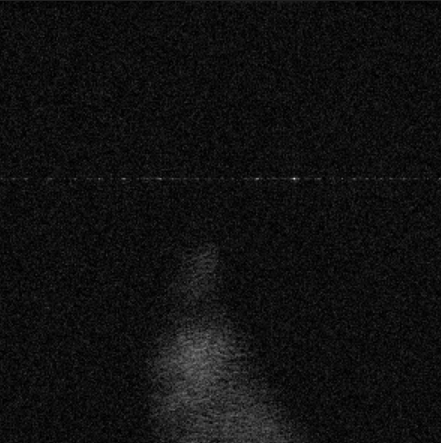
\includegraphics[width=\linewidth]{bad_slice.png}
        \caption{Example of a bad slice.}
        \label{fig:bad_slice}
    \end{minipage}%
    \hfill
    \begin{minipage}{0.45\textwidth}
        \centering
        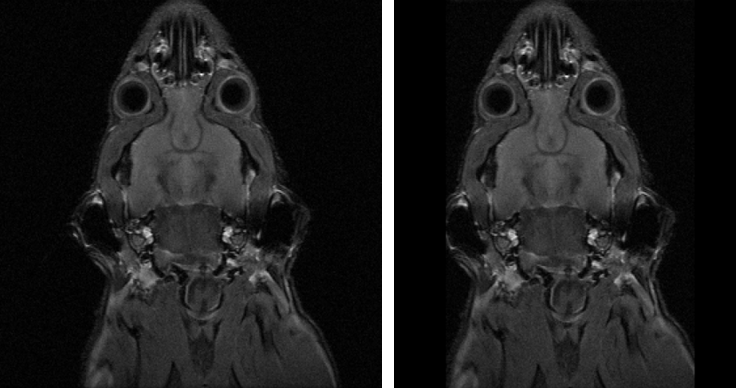
\includegraphics[width=\linewidth]{comparision cropped vs non cropped.png}
        \caption{The left figure shows the original slice, while the right figure is the cropped slice.}
        \label{fig:comparision-cropped}
    \end{minipage}
\end{figure}



\newpage

\section{Appendix: Mathematics APDDM}
\label{appendix:Mathematics APDDM}
\subsection{Ansatz: linear interpolation between image pair}
Some definitions:
\\
$\bold{x}_0$ = high-SNR image\\
$\bold{x}_T^*$ = low-SNR image (* denotes that this is the ground truth endpoint, the reason for this differentiation will be clear later)\\
$T$ = total amount of steps that will be taken\\
t = current timestep in the diffusion path \\
$\alpha_t = \frac{t}{T}$, notation for the fraction of the diffusion path at the current timestep\\
$\bold{R} = \bold{x}_T^* - \bold{x}_0$, the residual\\
\\
Note: $\bold{x}_0$ and $\bold{x}_T^*$ should be normalized images:
\begin{equation}
    \bold{x} \leftarrow \frac{\bold{x} - \frac{1}{i,j}\sum_{ij} \bold{x}_{ij}}{ \sqrt{ \frac{1}{ij} \sum_{i,j} \bold{x}_{ij}^2}}
\end{equation}
and $\bold{x}_T^*$ should be interpolated to match the size of $\bold{x}_0$.\\
\\
We will start by first defining a procedure, where we linearly interpolate between $\bold{x}_0$ and $\bold{x}_T^*$, and add a not yet specified noise term:
\begin{equation}
    x_t = (1-\alpha_t)\cdot\bold{x}_0 + \alpha_t\cdot\bold{x}_T^* + noise(t)
\end{equation}

\subsection{Proposition of the Markovian process}
We will now transform this into a Markovian process, by allowing the endpoint to not be exactly $\bold{x}_T$, but rather let the endpoint $\bold{x}_T$ be $\bold{x}_T^*$ in expected value.\\
\\
If we subtract $\bold{x}_t$ by $\bold{x}_{t-1}$, we get:
\begin{equation}
    \bold{x}_t - \bold{x}_{t-1} = \alpha_t (\bold{x}_T^* - \bold{x}_0) - \alpha_{t-1} (\bold{x}_T^* - \bold{x}_0) + noise
\end{equation}
$\Leftrightarrow$
\begin{equation}
    \bold{x}_t - \bold{x}_{t-1} = (\alpha_t - \alpha_{t-1}) \bold{R} + noise
\end{equation}
$\Leftrightarrow$
\begin{equation}
    \bold{x}_t = \bold{x}_{t-1} + \frac{1}{T} \bold{R} + noise
\end{equation}
By using a Markov process, we create a natural diffusion path from $\bold{x}_0$ to $\bold{x}_t$, where each step builds up on the previous one. 
We now define our final Markov process as: 
\begin{equation} \label{eq:f(t)}
    \boxed{\bold{x}_t = q(\bold{x}_{t-1}) = \bold{x}_{t-1} + \frac{1}{T} \bold{R} + f(t) \hat{\epsilon} \hspace{.1cm};\hspace{.5cm} t=1,2,...,T}
\end{equation}

Where we define $f(\alpha_t)$ to be a function that is zero for arguments $0$ and $1$, and reaches a maximum of 1 somewhere in the range $[0,1]$. This is the noise schedule function. Let:
\begin{equation}
    f(t) = 4\alpha_t(1-\alpha_t) = 4 \frac{t}{T} (1-\frac{t}{T})
\end{equation}
This choice of function is arbitrary, but in this way, the noise term is gradually introduced and attenuated again so the course of the diffusion path has a natural way of going from starting point to endpoint. Below, the course of the variance throughout the path will be shown, where it will be clear why such a choice of attenuating noise schedule function is favorable. \\
\\
The noise term $\epsilon$ should be distributed according to the real noise in our data:
\begin{equation}
    \epsilon \sim P[noise]
\end{equation}
We will approximate this empirically by sampling from all the observed residuals in our dataset:
\begin{equation}
    \epsilon \approx \hat{\epsilon} \stackrel{i.i.d.}{\sim} \mathcal{E}_{dataset}
\end{equation}

This sampling of the noise residual can be done by i.i.d sampling residual bank $\mathcal{E}_{dataset}$. These are then rotated at random over 0°, 90°, 180° and 270° as an augmentation technique so coherent edge artifacts won't accumulate (see Fig. \ref{fig:edge artifacts} for an example of such artifacts). 

\begin{figure}[h!]
    \centering
    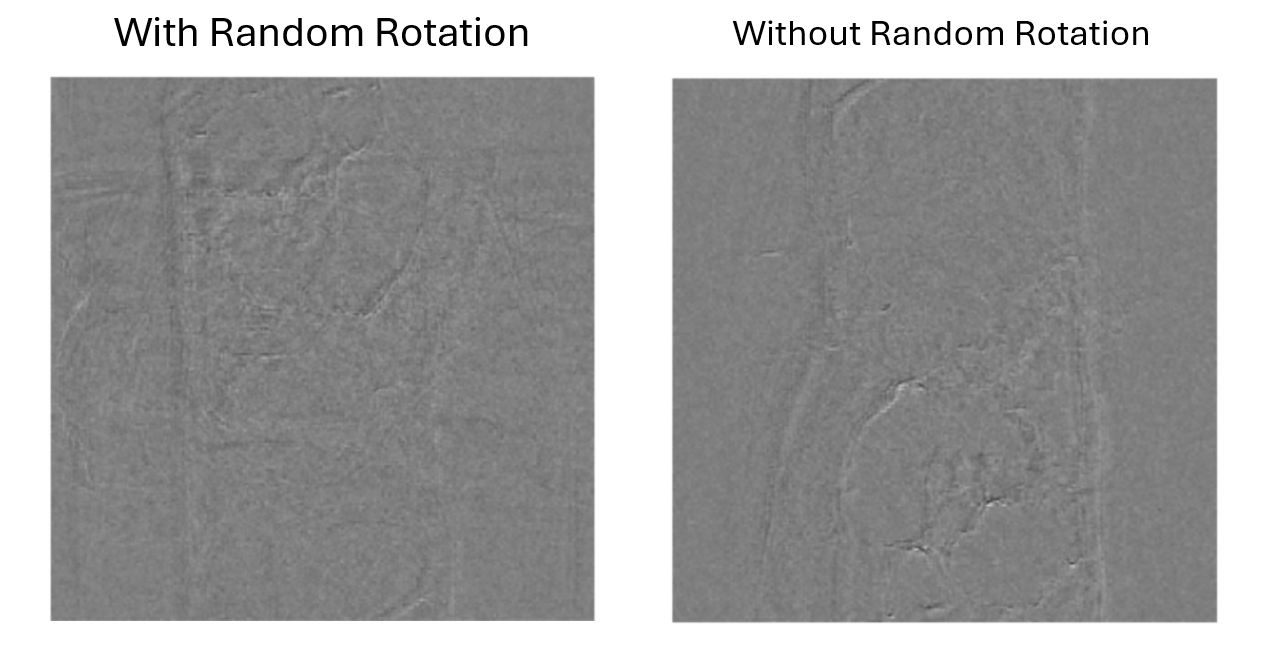
\includegraphics[width=0.8\linewidth]{With-Without_Random_Rotation.png}
    \caption{\textit{Demonstration of coherent edge artifact accumulation when no rotation is applied. }}
    \label{fig:edge artifacts}
\end{figure}

\FloatBarrier

\subsection{Expected value of the endpoint}
Note that generally: $\bold{x}_T \neq \bold{x}_T^*$. It will now be shown that the expected value $\mathbb{E}[\bold{x}_T]$ still is $\bold{x}_T^*$:\\
\\
We apply a Markov chain T times to the input $\bold{x}_0$:\\
\begin{equation}
    \mathbb{E}[\bold{x}_T] = \mathbb{E}[q(q(...q(\bold{x}_0)..))] = \mathbb{E}[\bold{x}_0 + \frac{T}{T} \bold{R} + \sum_{t=1}^{T} f(t) \cdot \hat{\epsilon}_t] 
\end{equation}
Because $\bold{R}= \bold{x}_T^* - \bold{x}_0$:
\begin{equation}
    \mathbb{E}[\bold{x}_T] = \mathbb{E}[\bold{x}_T^* + \sum_{t=1}^{T} f(t) \cdot \hat{\epsilon}_t] = \bold{x}_T^* + \sum_{t=1}^{T} f(t) \cdot \mathbb{E}[\hat{\epsilon}_t]
\end{equation}
If we assume $\mathbb{E}[\hat{\epsilon}] = 0$:
\begin{equation}
    \boxed{\mathbb{E}[\bold{x}_T] = \bold{x}_T^*}
\end{equation}

\subsection{Variance of the endpoint}
We will now derive the expression for the variance on our enpoint $\bold{x}_T$:
\begin{multline}
    Var[\bold{x}_T] = Var[q(q(...q(\bold{x}_0)..))] = Var[\bold{x}_0 + \bold{R} + \sum_{t=1}^{T} f(t) \cdot \hat{\epsilon}_t] = Var[\sum_{t=1}^{T} f(t) \cdot \hat{\epsilon}_t]\\ = \sum_{t=1}^{T} f(t)^2 Var[\hat{\epsilon}_t] + \sum_{i \neq j}^{T} f(i) f(j) Cov[\hat{\epsilon}_i, \hat{\epsilon}_j] = \sum_{t=1}^{T} f(t)^2 Var[\hat{\epsilon}_t]
\end{multline}
Where we used $Cov[\hat{\epsilon}_i, \hat{\epsilon}_j] = 0$ because the noise samples are independent. \\
Now using the notation: $Var[\hat{\epsilon}_t] = \sigma_{\epsilon}^2$, and substituting (\ref{eq:f(t)}), we get:
\begin{equation}
    \boxed{Var[\bold{x}_T] = \sigma_{\epsilon}^2 \cdot \sum_{t=1}^{T} f(t)^2 = \frac{8}{15} \frac{T^4 - 1}{T^3} \cdot \sigma_{\epsilon}^2}
\end{equation}
Note that for $lim_{T->+\infty} Var[\bold{x}_T] \sim \frac{8}{15} T$.\\
\\
We can also derive the general variance throughout the whole path (not just at the endpoint):
\begin{equation}
    Var[\bold{x}_T] = \sigma_{\epsilon}^2 \cdot \sum_{\tau=1}^{T} f(\tau)^2 = \sigma_{\epsilon}^2 \cdot \frac{8}{15} \frac{1}{T^4} t(t+1)[6t^3 - 15t^2T + 9t^2 + 10tT^2 - 15tT + t + 5T^2 - 1]
\end{equation}
% plot -----------------------
\begin{center}
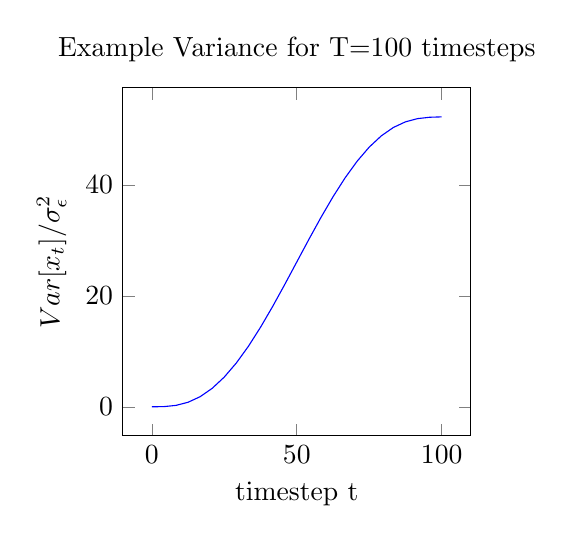
\begin{tikzpicture}
\begin{axis}[ylabel = {$Var[x_t] / \sigma_{\epsilon}^2$}, xlabel={timestep t}, title={Example Variance for T=100 timesteps}, width=6cm, height=6cm]
\addplot[color=blue, domain=0:100]{8/15 * x * (x-1) * 1/(100^4) * (6*x^3 - 15*x^2 * 100 + 9*x^2 + 10*x*100^2 - 15*x*100 + x + 5*100^2 - 1)};
\end{axis}
\end{tikzpicture}
\end{center}
This exact course of the variance has also been confirmed by numerical simulation.\\
\\
We can observe that the variance increases slowly in the beginning, and before the endpoint, it slows down and stabilizes again. This is the reason for the particular choice of the noise schedule function $f(t)$ discussed previously. \textbf{However, a lot of noise schedule choices can be made and should be investigated.}

\subsection{Controlling the variance}
I will now propose a method of controlling the variance of this path. This way, we can have the variance of the endpoint as a variable parameter, and even optimize the model in function of this parameter. Thus the ``degree of noise'' can be controlled.   
First, we will normalize the sampled residual $\hat{\epsilon}$, so we know the variance of the noise is 1:
\begin{equation}
    \hat{\epsilon'} = \hat{\epsilon} / s_{n,\epsilon}
\end{equation}
($s_{n,\epsilon}$ = population variance of $\mathcal{E}_{dataset}$)\\
Additional note: we assume that an empirical noise distribution has an expected value of 0.\\
We will then control the variance by adding a parameter $\sigma$:
\begin{equation}
    \boxed{\bold{x}_t = q(\bold{x}_{t-1}) = \bold{x}_{t-1} + \frac{1}{T} \bold{R} + \sigma f(t) \hat{\epsilon'} \hspace{.1cm};\hspace{.5cm} t=1,2,...,T}
\end{equation}
Where: 
\begin{equation} \label{eq:beta}
    \sigma = \sqrt{\frac{15}{8} * \frac{T^3}{T^4 - 1}} * \beta
\end{equation}
Now, the variance of our endpoint is: 
\begin{equation}
    Var[\bold{x}_T] = \beta^2
\end{equation}
We now have full control over the variance of the endpoint, with exception to the stability criterion as described in the following section. 

\subsection{MSE stability}
Important to note is that there are some constraints on this parameter beta (and thus the variance of the noise term), if we want the diffusion path to converge to $\bold{X}_T^*$. We will measure this in the form of the MSE between $\bold{x}_T$ and $\bold{x}_T^*$, which should not be exceedingly large. \\
An important condition that must be met, is that $\bold{x}_t$ becomes more similar to $\bold{x}_T^*$ each step.\\
\\
 This condition will not be met if the noise term overpowers the term $\frac{1}{T}  \bold{R}$ at a certain step. In other words, the residual term magnitude should be larger than the noise term magnitude in each step, so that the diffusion path still mostly converges towards $x_T^*$. We will make an estimation of the size of the subsequent terms based on their Mean Square value $\frac{1}{i,j}\sum_{i,j} X_{i,j}^2$ (MS value). We will also let $f(t) = 1$, to have a conservative estimation.  \\
 The diffusion path will converge if for all steps:
\begin{equation}
    \mathbb{E}[MS(\hat{\epsilon})] \lesssim MS(\frac{1}{T} \bold{R})
\end{equation}
$\Leftrightarrow$
 \begin{equation}
    \sigma^2 \cdot MS(\mathbb{E}[\hat{\epsilon}']) \lesssim \frac{1}{T^2} MS(\bold{R})
\end{equation}
$\Leftrightarrow$
 \begin{equation}
    \boxed{\sigma \lesssim \frac{1}{T} RMS(\bold{R}) = \sigma_{crit}}
\end{equation}
This last expression is a conservative MSE convergence condition. \\
Substituting (\ref{eq:beta}), we get the criterion in terms of $\beta$:
\begin{equation}
    \beta \lesssim \sqrt{\frac{8}{15} \frac{T^4-1}{T^5}} RMS(\bold{R}) = \beta_{crit}
\end{equation}
\\
This result can be demonstrated by a simulation where beta is varied and the mean square error between $x_T$ and $x_T^*$ is computed over N diffusion path samples (Fig. \ref{fig:beta sweep}). We indeed observe that if $\beta$ is within the order of magnitude of $\beta_{crit}$, the diffusion process won't converge towards $x_T^*$ anymore, which manifests itself in an increase in the MSE. 
\begin{figure}[h!]
    \centering
    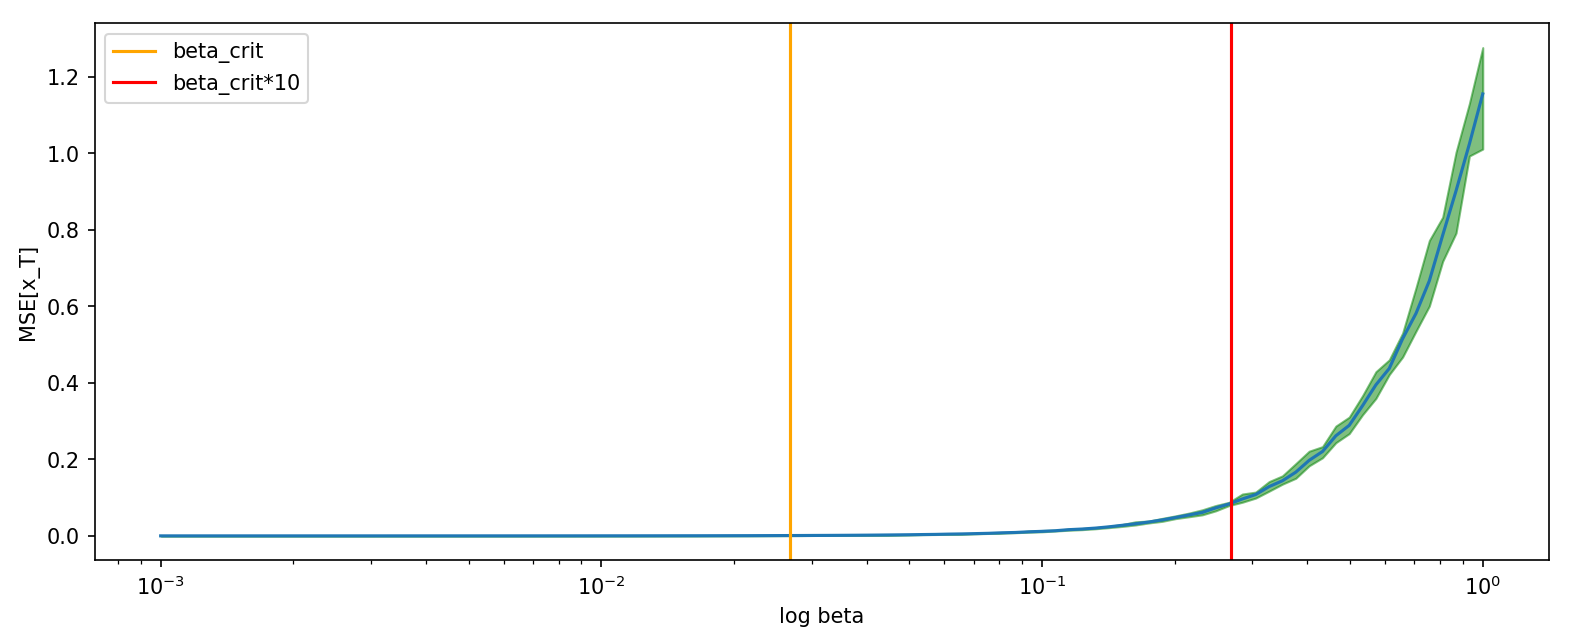
\includegraphics[width=0.8\linewidth]{beta_sweep.png}
    \caption{\textit{Plot of $MSE(x_T, x_T^*)$ against beta. }}
    \label{fig:beta sweep}
\end{figure}

\FloatBarrier

\clearpage
\newpage
\section{Appendix: Figures Results}
\subsection{Appendix: first results}
\label{Appendix: first results}
\begin{figure*}[h]
    \centering
    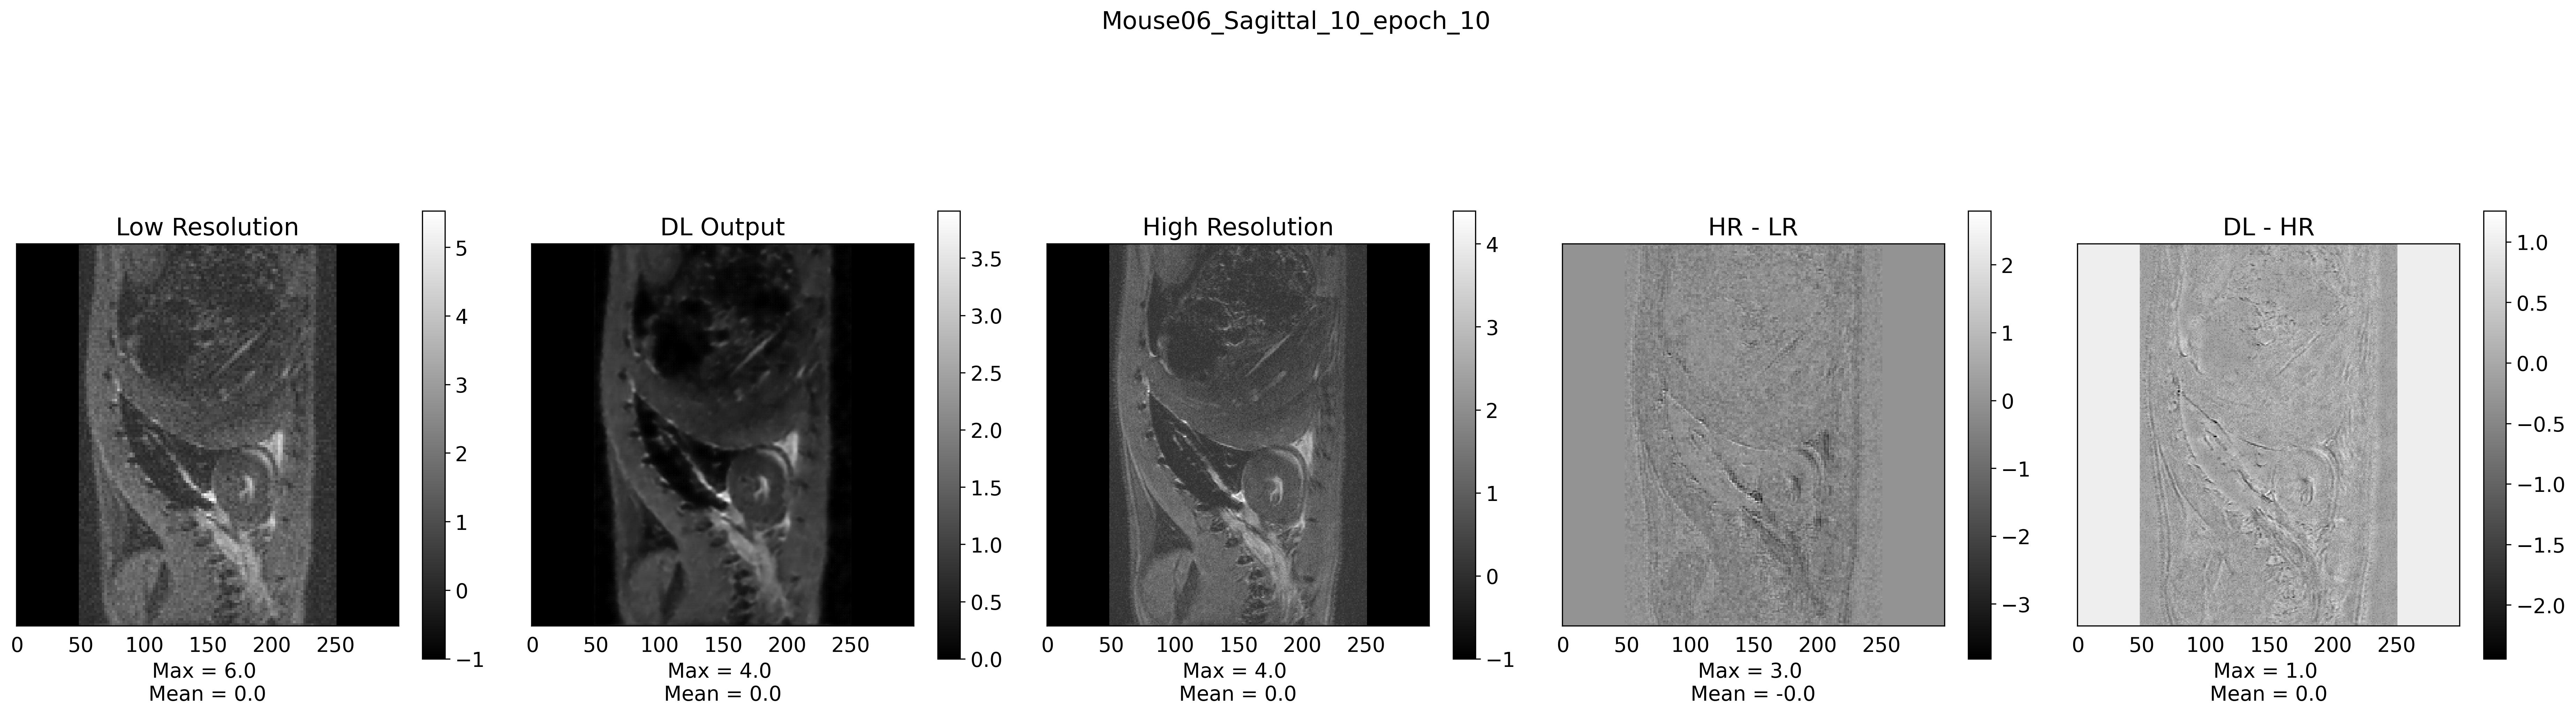
\includegraphics[width=1\linewidth]{Mouse06_Sagittal_10_epoch_10.png}
    \caption{First results of abdomen of test mouse.}
\end{figure*}

\begin{figure*}[h]
    \centering
    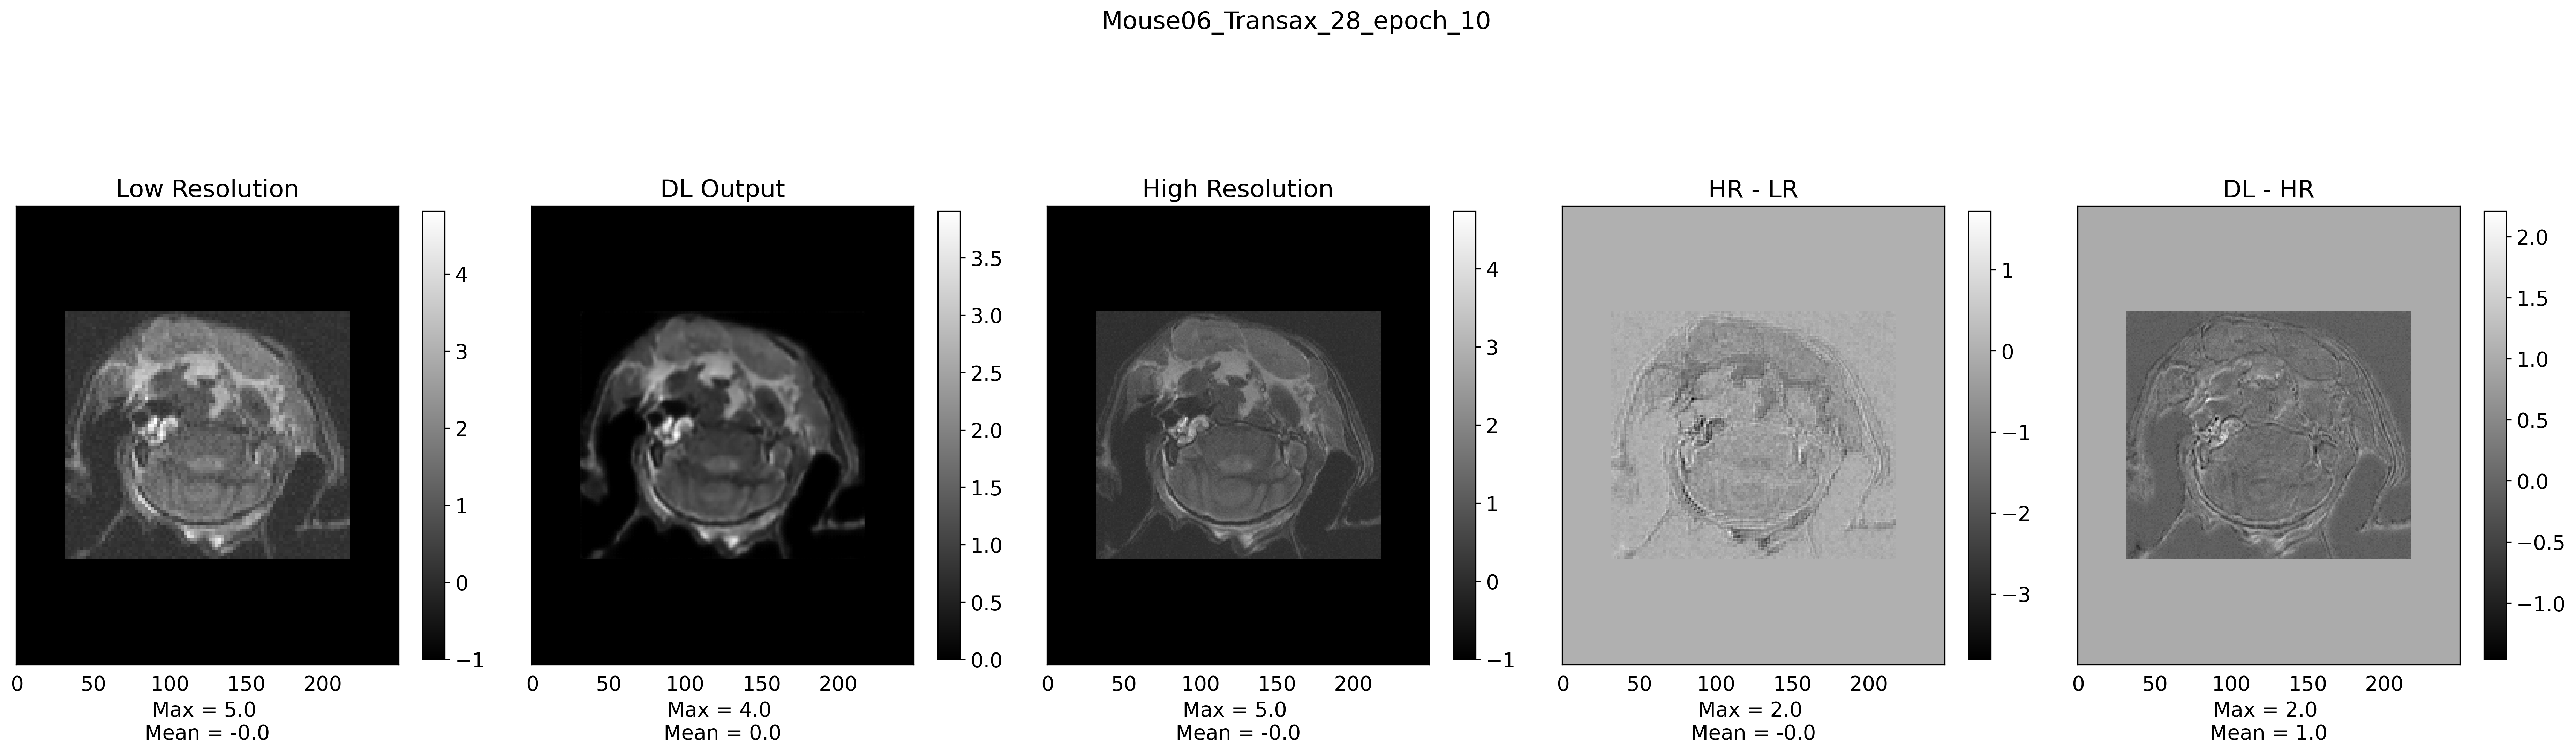
\includegraphics[width=1\linewidth]{Mouse06_Transax_28_epoch_10.png}
    \caption{First results of abdomen of test mouse.}
\end{figure*}

\begin{figure*}[h]
    \centering
    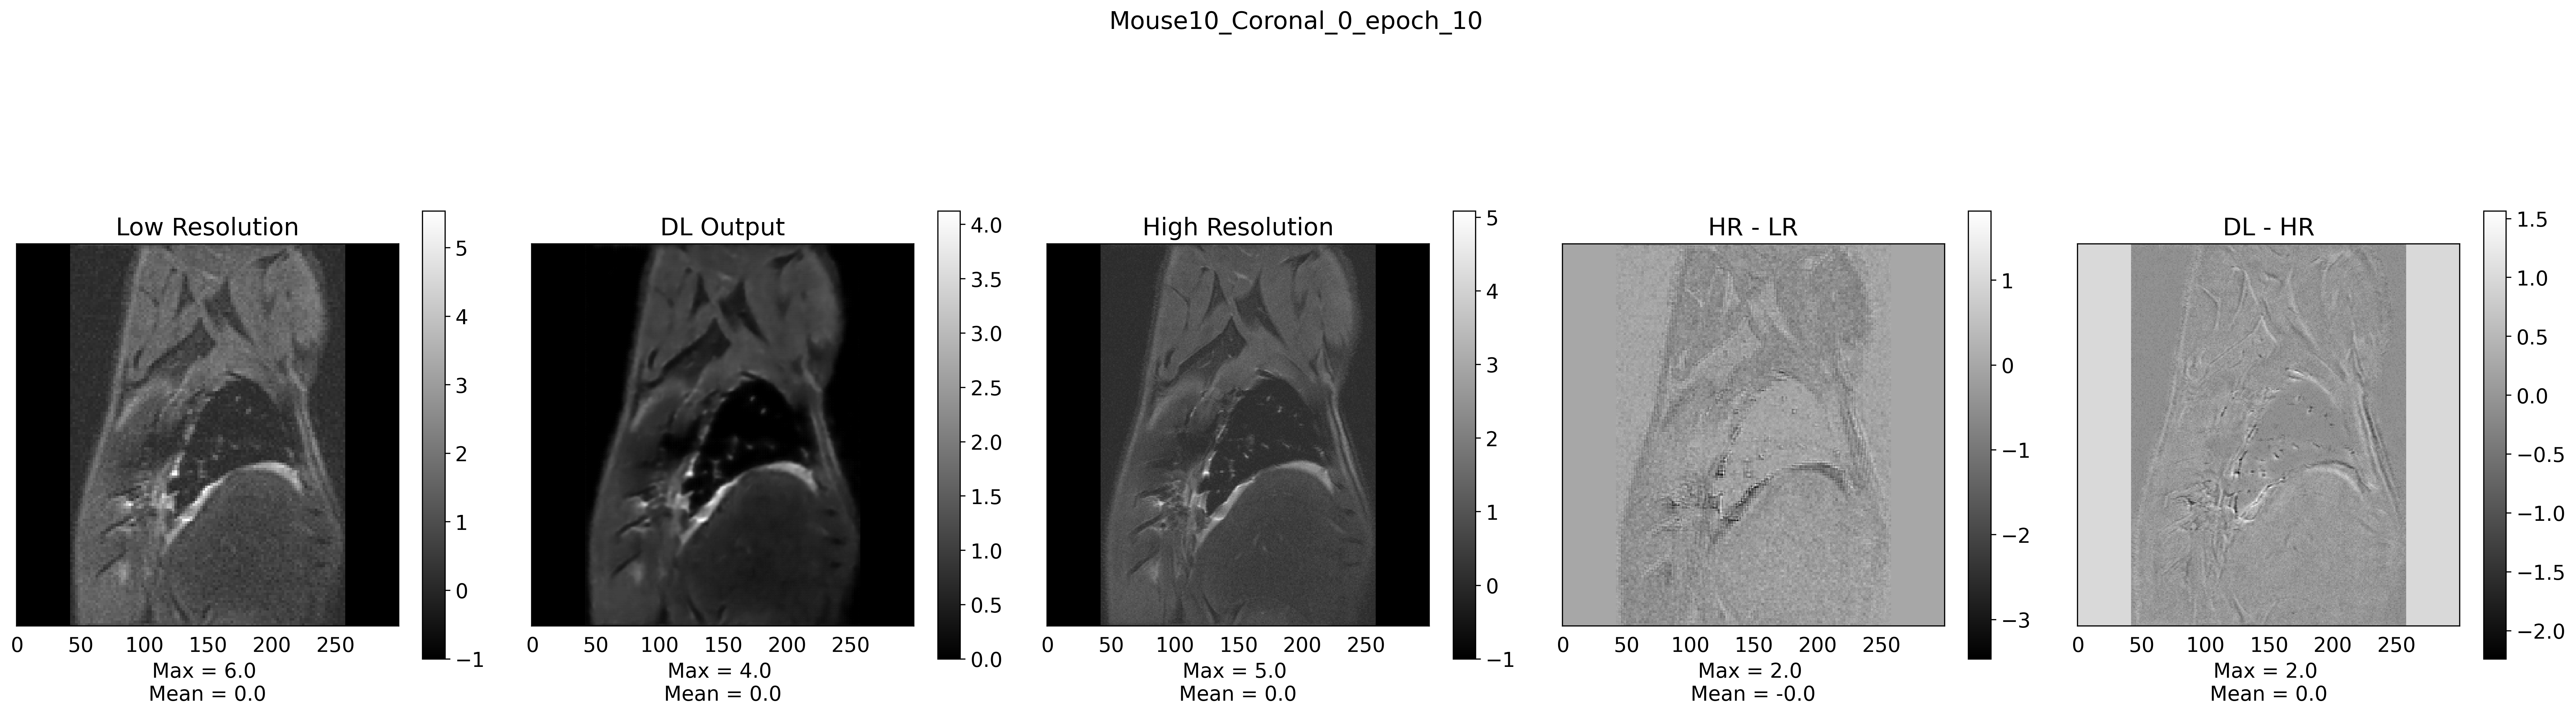
\includegraphics[width=1\linewidth]{Mouse10_Coronal_0_epoch_10.png}
    \caption{First results of abdomen of test mouse.}
\end{figure*}

\newpage
\subsection{Appendix: results after hyperparameter tuning}
\label{Appendix: results after tuning}
\begin{figure*}[h]
    \centering
    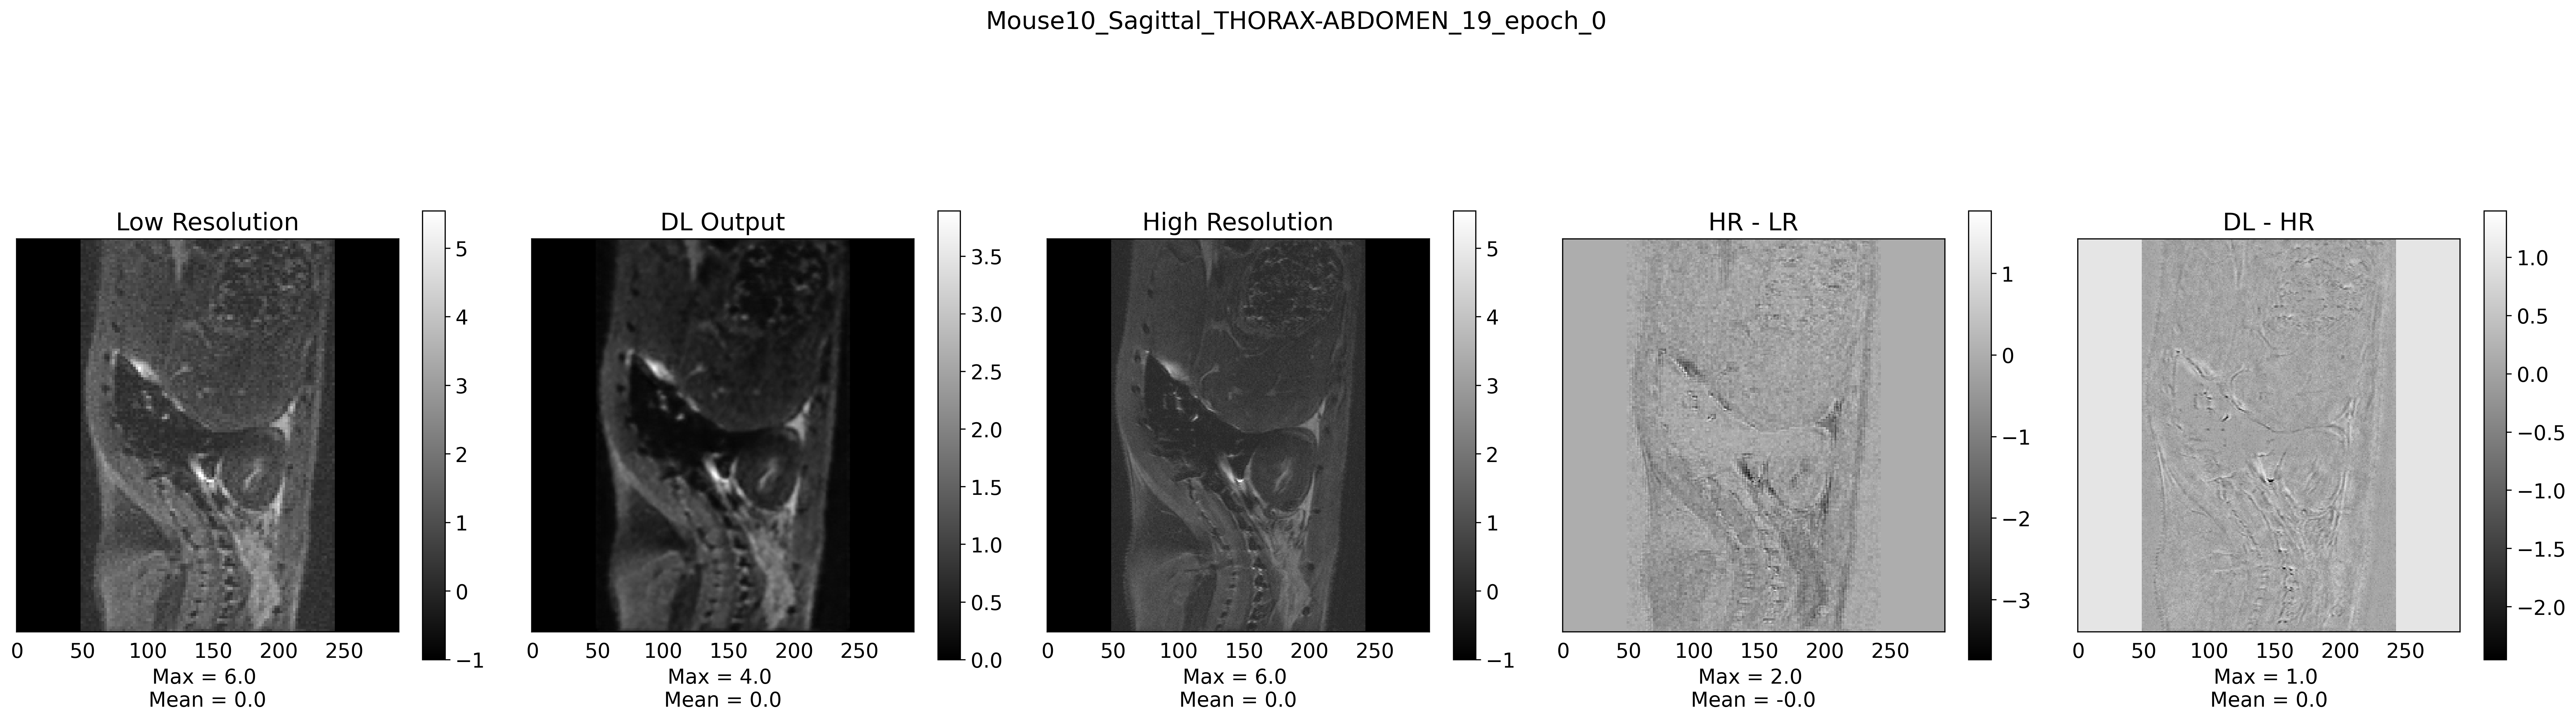
\includegraphics[width=1\linewidth]{Mouse10_Sagittal_THORAX-ABDOMEN_19_epoch_0.png}
    \caption{Results after hyperparameter tuning of abdomen of test mouse.}
    \label{mouse10_s_19}
\end{figure*}

\begin{figure*}[h]
    \centering
    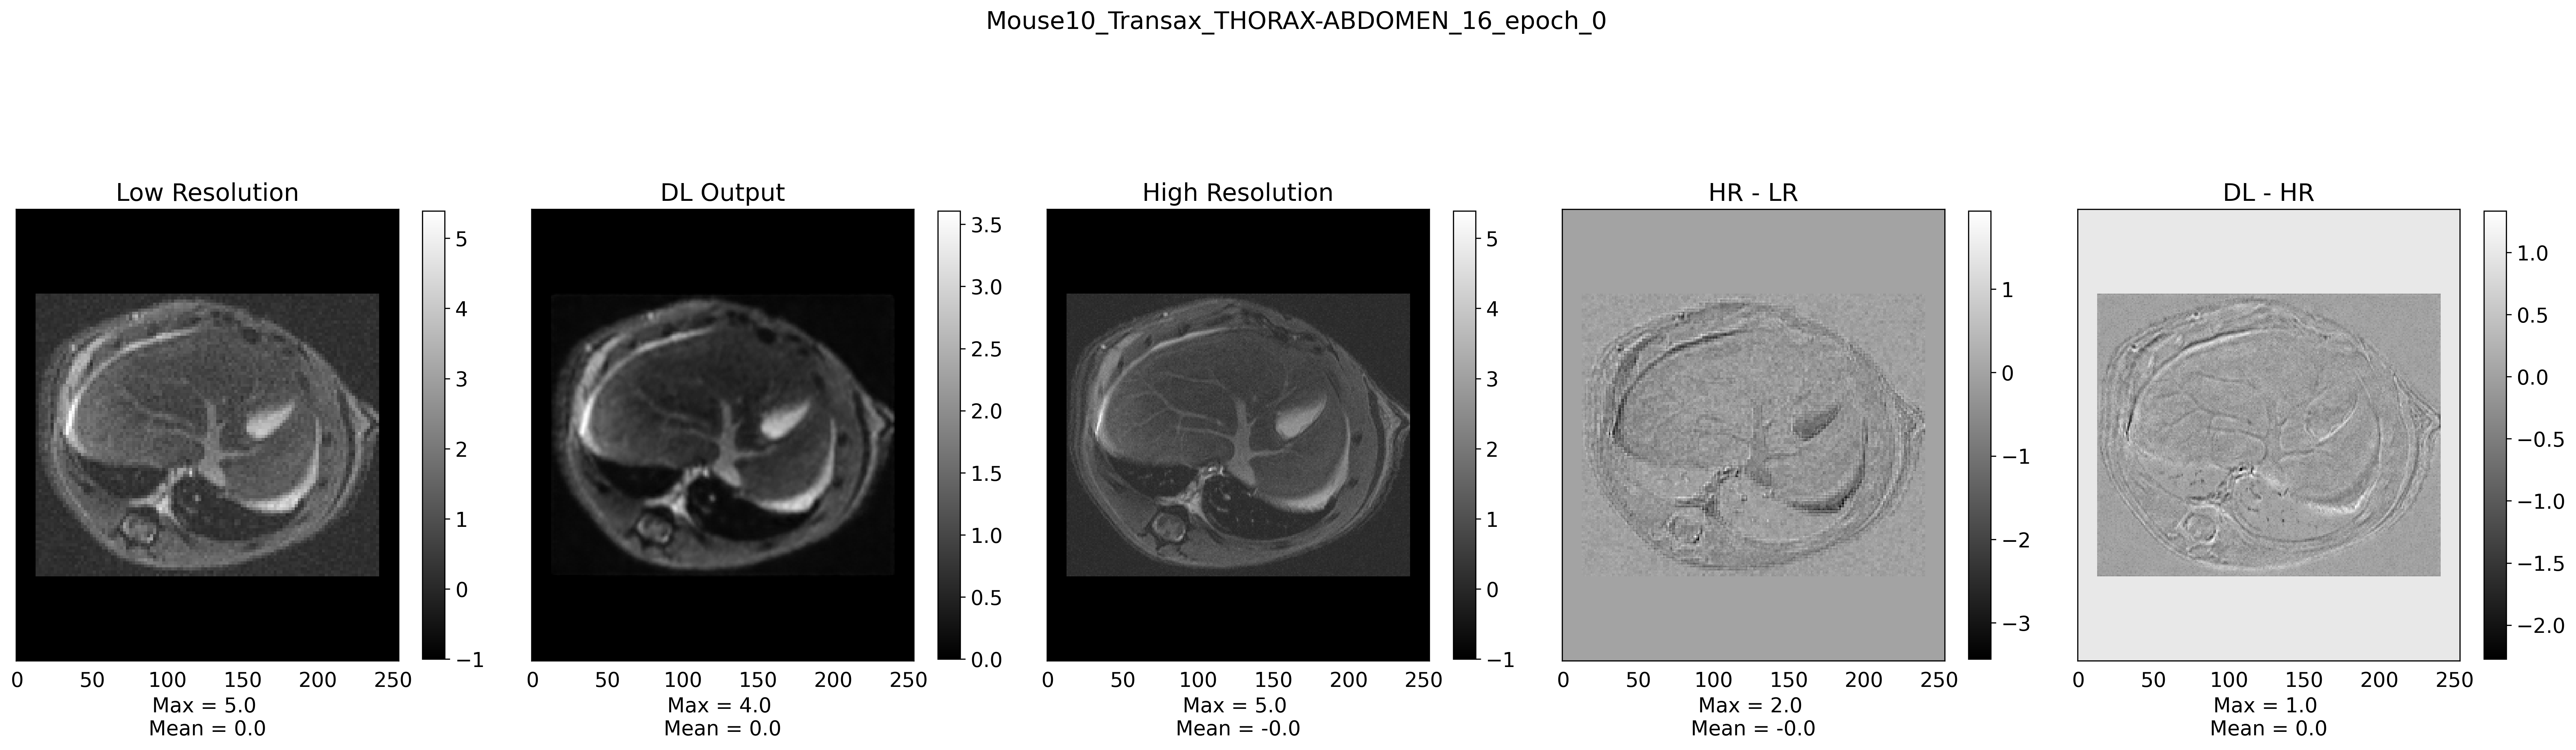
\includegraphics[width=1\linewidth]{Mouse10_Transax_THORAX-ABDOMEN_16_epoch_0.png}
    \caption{Results after hyperparameter tuning of abdomen of test mouse.}
    \label{mouse10_t_16}
\end{figure*}

\begin{figure*}[h]
    \centering
    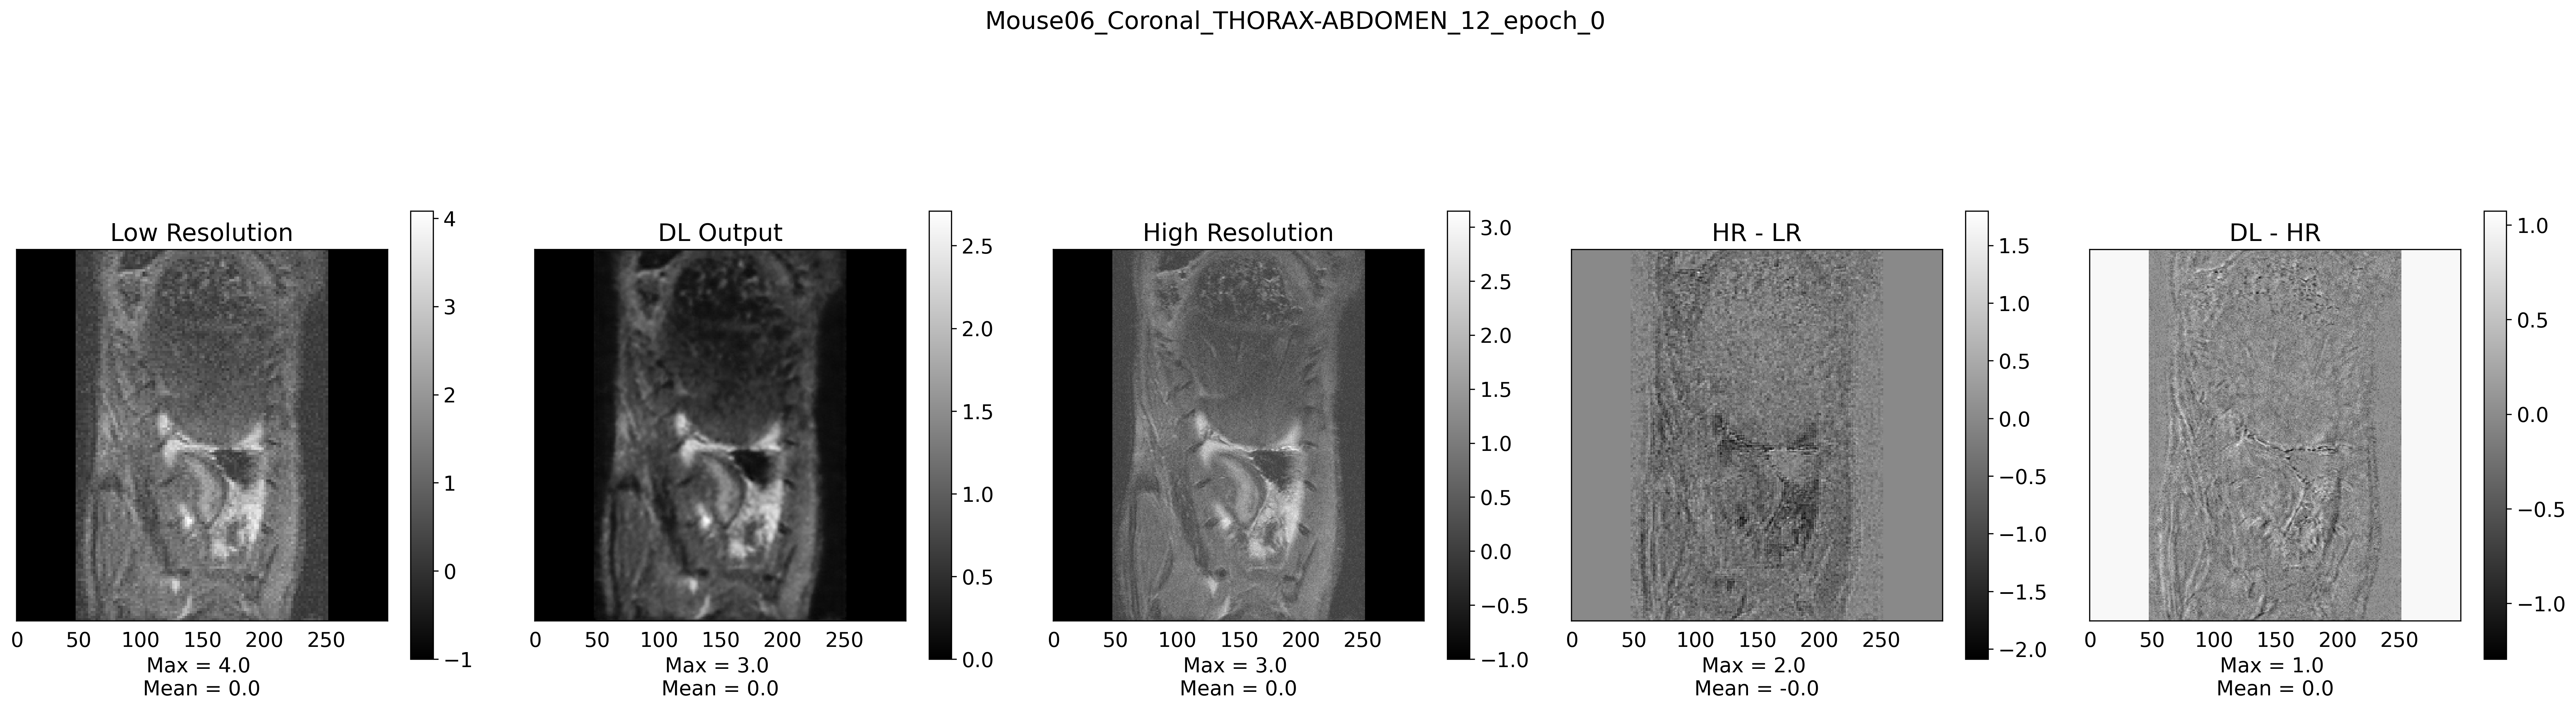
\includegraphics[width=1\linewidth]{Mouse06_Coronal_THORAX-ABDOMEN_12_epoch_0.png}
    \caption{Results after hyperparameter tuning of abdomen of test mouse.}
    \label{mouse06_c_12}
\end{figure*}

\section{Appendix: Validation}\label{Appendix: val}
\begin{sidewaystable}[h]
    \centering
    \caption{Overview of the mice, slices and planes used to obtain CNR and normalised variance in LR, DL and HR images. TA stands for thorax-abdomen, while HT is used for head-thorax.}
    \resizebox{0.8\linewidth}{!}{
    \begin{tabular}{l|c|c|c|c|c|c|c|c|c|c|c|c|c|c|c|c|c|c|c|c|c|c}
    \toprule
     & \textbf{Mouse} & \textbf{Plane} & \textbf{Slice} & \textbf{Region} &&\textbf{LR mean ROI} &\textbf{LR mean background} &\textbf{LR STD background}&\textbf{LR CNR}& \textbf{LR normalised variance} & &\textbf{DL mean ROI} &\textbf{DL mean background} &\textbf{DL STD background}&\textbf{DL CNR}&\textbf{DL normalised variance} &&\textbf{HR mean ROI} &\textbf{HR mean background} &\textbf{HR STD background}&\textbf{HR CNR}& \textbf{HR normalised variance} \\
    \midrule
     & 1  & Sagittal   & 6&TA           &   &1.103&0.212&0.121&0.736&0.571       &          &0.690&0.152&0.017&31.441&0.112           &      &0.883&0.188&0.105&6.616&0.558                   \\
     &    & Transaxial & 13&TA          &   &0.866&3.319&0.016&-155.242&0.005      &        &0.581&2.312&0.002&-706.785&0.001         &      &0.565&2.288&0.006&-270.741&0.003                   \\
     &    & Coronal    & 10&TA          &   &0.725&2.912&0.149&-14.699&0.051     &          &0.527&1.933&0.003&-426.689&0.002         &      &0.529&2.112&0.009&-179.984&0.004                   \\
    \midrule
     & 23 & Sagittal   & 10&TA          &   &0.574&2.482&0.247&-7.27&0.099        &         &0.433&1.673&0.159&-7.777&0.095          &       &0.616&2.676&0.153&-13.441&0.057                   \\
     &    & Transaxial & 4&TA           &   &1.410&2.104&0.191&-3.623&0.091       &         &0.909&1.409&0.114&-4.408&0.081          &       &1.400&2.165&0.280&-2.7929&0.130                   \\
     &    & Coronal    & 22&HT          &   &2.421&1.094&0.168&7.901&0.153         &        &1.634&0.696&0.055&16.972&0.800          &       &2.211&0.915&0.122&10.589&0.134                   \\
    \midrule
     & 6 & Sagittal    & 10&TA           &  &1.187&0.459&0.206&3.530&0.449          &       &0.811&0.193&0.020&31.358&0.102           &      &0.743&0.220&0.145&3.609&0.657                   \\
     &    & Transaxial & 21&HT          &   &2.471&1.220&0.146&8.592&0.119         &        &1.817&0.791&0.031&0.031&0.040           &       &1.629&0.752&0.118&7.453&0.157                   \\
     &    & Coronal    & 7&TA            &  &0.270&0.930&0.174&-3.783&0.188         &       &0.174&0.606&0.041&-10.655&0.067          &      &0.181&0.684&0.123&-4.075&0.180                   \\
    \midrule
     & 10 & Sagittal   & 11&TA          &   &0.235&0.660&0.180&-2.354&0.273         &       &0.144&0.451&0.074&-4.146&0.0164          &      &0.135&0.437&0.114&-2.650&0.260                   \\
     &    & Transaxial & 22&HT          &   &1.125&1.871&0.093&-7.994&0.045         &       &0.763&1.313&0.042&-13.058&0.032         &       &0.718&1.195&0.080&-6.006&0.067                   \\
     &    & Coronal    & 5&TA           &   &0.234&2.204&0.196&-9.144&0.097          &      &0.142&1.377&0.097&-12.715&0.071         &       &0.129&1.348&0.154&-7.891&0.115                   \\
    \midrule
     & 7  & Sagittal   & 11&TA         &    &0.264&1.032&0.268&-2.870&0.259          &      &0.159&0.617&0.081&-5.628&0.132          &       &0.189&0.610&0.160&-2.630&0.263                   \\
     &    & Transaxial & 12&TA         &    &0.294&1.091&0.185&-4.304&0.170         &       &0.168&0.695&0.057&-9.234&0.082         &        &0.192&0.856&0.150&-4.427&0.175                   \\
     &    & Coronal    & 11&TA          &   &0.297&0.576&0.166&-1.678&0.288         &       &0.154&0.407&0.050&-5.069&0.123          &       &0.0161&0.446&0.102&-2.797&0.228                   \\
    \midrule
     & 22 & Sagittal   & 12&HT         &    &0.213&2.469&0.246&-8.559&0.107         &       &0.128&1.701&0.153&-10.269&0.090        &        &0.160&1.956&0.176&-10.207&0.090                   \\
     &    & Transaxial & 8&TA           &   &0.771&1.843&0.351&-3.057&0.190          &      &0.514&1.296&0.195&-4.004&0.151         &        &0.628&1.438&0.273&-2.971&0.190                   \\
     &    & Coronal    & 13&TA         &    &0.204&1.153&0.215&-4.414&0.187          &      &0.130&0.740&0.084&-7.264&0.113         &        &0.221&0.972&0.183&-4.101&0.188                   \\
     \bottomrule
    \end{tabular}
    }
\end{sidewaystable}

\end{appendices}

\end{document}
